\documentclass[]{book}
\usepackage{lmodern}
\usepackage{amssymb,amsmath}
\usepackage{ifxetex,ifluatex}
\usepackage{fixltx2e} % provides \textsubscript
\ifnum 0\ifxetex 1\fi\ifluatex 1\fi=0 % if pdftex
  \usepackage[T1]{fontenc}
  \usepackage[utf8]{inputenc}
\else % if luatex or xelatex
  \ifxetex
    \usepackage{mathspec}
  \else
    \usepackage{fontspec}
  \fi
  \defaultfontfeatures{Ligatures=TeX,Scale=MatchLowercase}
\fi
% use upquote if available, for straight quotes in verbatim environments
\IfFileExists{upquote.sty}{\usepackage{upquote}}{}
% use microtype if available
\IfFileExists{microtype.sty}{%
\usepackage{microtype}
\UseMicrotypeSet[protrusion]{basicmath} % disable protrusion for tt fonts
}{}
\usepackage[margin=1in]{geometry}
\usepackage{hyperref}
\hypersetup{unicode=true,
            pdftitle={Statistics 1},
            pdfborder={0 0 0},
            breaklinks=true}
\urlstyle{same}  % don't use monospace font for urls
\usepackage{color}
\usepackage{fancyvrb}
\newcommand{\VerbBar}{|}
\newcommand{\VERB}{\Verb[commandchars=\\\{\}]}
\DefineVerbatimEnvironment{Highlighting}{Verbatim}{commandchars=\\\{\}}
% Add ',fontsize=\small' for more characters per line
\usepackage{framed}
\definecolor{shadecolor}{RGB}{248,248,248}
\newenvironment{Shaded}{\begin{snugshade}}{\end{snugshade}}
\newcommand{\KeywordTok}[1]{\textcolor[rgb]{0.13,0.29,0.53}{\textbf{#1}}}
\newcommand{\DataTypeTok}[1]{\textcolor[rgb]{0.13,0.29,0.53}{#1}}
\newcommand{\DecValTok}[1]{\textcolor[rgb]{0.00,0.00,0.81}{#1}}
\newcommand{\BaseNTok}[1]{\textcolor[rgb]{0.00,0.00,0.81}{#1}}
\newcommand{\FloatTok}[1]{\textcolor[rgb]{0.00,0.00,0.81}{#1}}
\newcommand{\ConstantTok}[1]{\textcolor[rgb]{0.00,0.00,0.00}{#1}}
\newcommand{\CharTok}[1]{\textcolor[rgb]{0.31,0.60,0.02}{#1}}
\newcommand{\SpecialCharTok}[1]{\textcolor[rgb]{0.00,0.00,0.00}{#1}}
\newcommand{\StringTok}[1]{\textcolor[rgb]{0.31,0.60,0.02}{#1}}
\newcommand{\VerbatimStringTok}[1]{\textcolor[rgb]{0.31,0.60,0.02}{#1}}
\newcommand{\SpecialStringTok}[1]{\textcolor[rgb]{0.31,0.60,0.02}{#1}}
\newcommand{\ImportTok}[1]{#1}
\newcommand{\CommentTok}[1]{\textcolor[rgb]{0.56,0.35,0.01}{\textit{#1}}}
\newcommand{\DocumentationTok}[1]{\textcolor[rgb]{0.56,0.35,0.01}{\textbf{\textit{#1}}}}
\newcommand{\AnnotationTok}[1]{\textcolor[rgb]{0.56,0.35,0.01}{\textbf{\textit{#1}}}}
\newcommand{\CommentVarTok}[1]{\textcolor[rgb]{0.56,0.35,0.01}{\textbf{\textit{#1}}}}
\newcommand{\OtherTok}[1]{\textcolor[rgb]{0.56,0.35,0.01}{#1}}
\newcommand{\FunctionTok}[1]{\textcolor[rgb]{0.00,0.00,0.00}{#1}}
\newcommand{\VariableTok}[1]{\textcolor[rgb]{0.00,0.00,0.00}{#1}}
\newcommand{\ControlFlowTok}[1]{\textcolor[rgb]{0.13,0.29,0.53}{\textbf{#1}}}
\newcommand{\OperatorTok}[1]{\textcolor[rgb]{0.81,0.36,0.00}{\textbf{#1}}}
\newcommand{\BuiltInTok}[1]{#1}
\newcommand{\ExtensionTok}[1]{#1}
\newcommand{\PreprocessorTok}[1]{\textcolor[rgb]{0.56,0.35,0.01}{\textit{#1}}}
\newcommand{\AttributeTok}[1]{\textcolor[rgb]{0.77,0.63,0.00}{#1}}
\newcommand{\RegionMarkerTok}[1]{#1}
\newcommand{\InformationTok}[1]{\textcolor[rgb]{0.56,0.35,0.01}{\textbf{\textit{#1}}}}
\newcommand{\WarningTok}[1]{\textcolor[rgb]{0.56,0.35,0.01}{\textbf{\textit{#1}}}}
\newcommand{\AlertTok}[1]{\textcolor[rgb]{0.94,0.16,0.16}{#1}}
\newcommand{\ErrorTok}[1]{\textcolor[rgb]{0.64,0.00,0.00}{\textbf{#1}}}
\newcommand{\NormalTok}[1]{#1}
\usepackage{longtable,booktabs}
\usepackage{graphicx,grffile}
\makeatletter
\def\maxwidth{\ifdim\Gin@nat@width>\linewidth\linewidth\else\Gin@nat@width\fi}
\def\maxheight{\ifdim\Gin@nat@height>\textheight\textheight\else\Gin@nat@height\fi}
\makeatother
% Scale images if necessary, so that they will not overflow the page
% margins by default, and it is still possible to overwrite the defaults
% using explicit options in \includegraphics[width, height, ...]{}
\setkeys{Gin}{width=\maxwidth,height=\maxheight,keepaspectratio}
\IfFileExists{parskip.sty}{%
\usepackage{parskip}
}{% else
\setlength{\parindent}{0pt}
\setlength{\parskip}{6pt plus 2pt minus 1pt}
}
\setlength{\emergencystretch}{3em}  % prevent overfull lines
\providecommand{\tightlist}{%
  \setlength{\itemsep}{0pt}\setlength{\parskip}{0pt}}
\setcounter{secnumdepth}{5}
% Redefines (sub)paragraphs to behave more like sections
\ifx\paragraph\undefined\else
\let\oldparagraph\paragraph
\renewcommand{\paragraph}[1]{\oldparagraph{#1}\mbox{}}
\fi
\ifx\subparagraph\undefined\else
\let\oldsubparagraph\subparagraph
\renewcommand{\subparagraph}[1]{\oldsubparagraph{#1}\mbox{}}
\fi

%%% Use protect on footnotes to avoid problems with footnotes in titles
\let\rmarkdownfootnote\footnote%
\def\footnote{\protect\rmarkdownfootnote}

%%% Change title format to be more compact
\usepackage{titling}

% Create subtitle command for use in maketitle
\newcommand{\subtitle}[1]{
  \posttitle{
    \begin{center}\large#1\end{center}
    }
}

\setlength{\droptitle}{-2em}
  \title{Statistics 1}
  \pretitle{\vspace{\droptitle}\centering\huge}
  \posttitle{\par}
  \author{}
  \preauthor{}\postauthor{}
  \date{}
  \predate{}\postdate{}


\usepackage{amsthm}
\newtheorem{theorem}{Theorem}[chapter]
\newtheorem{lemma}{Lemma}[chapter]
\theoremstyle{definition}
\newtheorem{definition}{Definition}[chapter]
\newtheorem{corollary}{Corollary}[chapter]
\newtheorem{proposition}{Proposition}[chapter]
\theoremstyle{definition}
\newtheorem{example}{Example}[chapter]
\theoremstyle{definition}
\newtheorem{exercise}{Exercise}[chapter]
\theoremstyle{remark}
\newtheorem*{remark}{Remark}
\newtheorem*{solution}{Solution}
\begin{document}
\maketitle

{
\setcounter{tocdepth}{1}
\tableofcontents
}
\chapter*{About this course}\label{about-this-course}
\addcontentsline{toc}{chapter}{About this course}

This course is an introduction to data science. We have three primary
aims. First, to introduce you to the logic of quantitative research
design. Second, to familiarise you with statistical models that
scientists and policy-makers use to answer social science questions.
Third, to help you acquire the necessary skills to conduct your own
quantitative research projects. No prior statistical knowledge is
assumed. We will use the statistical software R and RStudio on top.

\begin{center}\rule{0.5\linewidth}{\linethickness}\end{center}

Syllabus

Moodle

Piazza

\chapter{Introduction: Measurement, Central Tendency, Dispersion,
Validity,
Reliability}\label{introduction-measurement-central-tendency-dispersion-validity-reliability}

\section{Seminar}\label{seminar}

In this seminar session, we introduce working with R. We illustrate some
basic functionality and help you familiarise yourself with the look and
feel of RStudio. Measures of central tendency and dispersion are easy to
calculate in R. We focus on introducing the logic of R first and then
describe how central tendency and dispersion are calculated in the end
of the seminar.

\subsection{Getting Started}\label{getting-started}

Install R and RStudio on your computer by downloading them from the
following sources:

\begin{itemize}
\tightlist
\item
  Download R from \href{https://cran.r-project.org}{The Comprehensive R
  Archive Network (CRAN)}
\item
  Download RStudio from \href{https://www.rstudio.com}{RStudio.com}
\end{itemize}

\subsection{RStudio}\label{rstudio}

Let's get acquainted with R. When you start RStudio for the first time,
you'll see three panes:

\begin{figure}
\centering
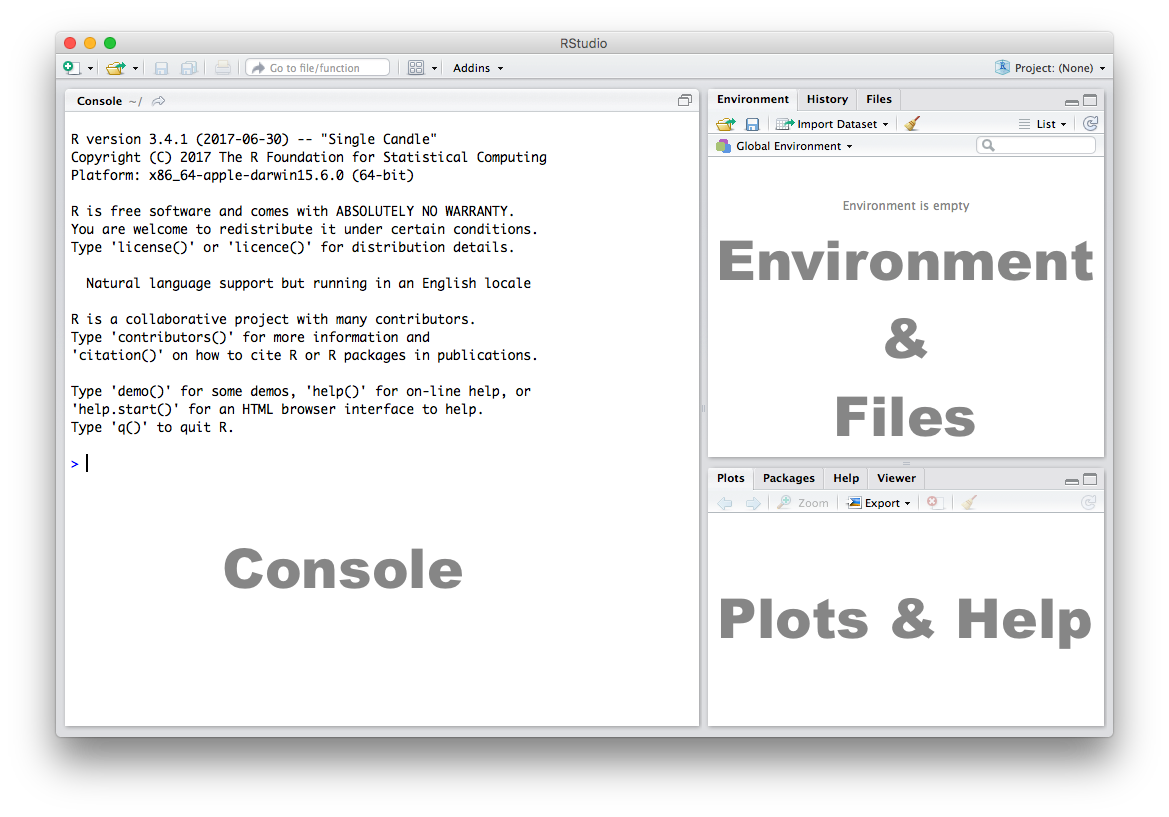
\includegraphics{./img/rstudio_default.png}
\caption{}
\end{figure}

\subsection{Console}\label{console}

The Console in RStudio is the simplest way to interact with R. You can
type some code at the Console and when you press ENTER, R will run that
code. Depending on what you type, you may see some output in the Console
or if you make a mistake, you may get a warning or an error message.

Let's familiarize ourselves with the console by using R as a simple
calculator:

\begin{Shaded}
\begin{Highlighting}[]
\DecValTok{2} \OperatorTok{+}\StringTok{ }\DecValTok{4}
\end{Highlighting}
\end{Shaded}

\begin{verbatim}
[1] 6
\end{verbatim}

Now that we know how to use the \texttt{+} sign for addition, let's try
some other mathematical operations such as subtraction (\texttt{-}),
multiplication (\texttt{*}), and division (\texttt{/}).

\begin{Shaded}
\begin{Highlighting}[]
\DecValTok{10} \OperatorTok{-}\StringTok{ }\DecValTok{4}
\end{Highlighting}
\end{Shaded}

\begin{verbatim}
[1] 6
\end{verbatim}

\begin{Shaded}
\begin{Highlighting}[]
\DecValTok{5} \OperatorTok{*}\StringTok{ }\DecValTok{3}
\end{Highlighting}
\end{Shaded}

\begin{verbatim}
[1] 15
\end{verbatim}

\begin{Shaded}
\begin{Highlighting}[]
\DecValTok{7} \OperatorTok{/}\StringTok{ }\DecValTok{2}
\end{Highlighting}
\end{Shaded}

\begin{verbatim}
[1] 3.5
\end{verbatim}

\begin{longtable}[]{@{}ll@{}}
\toprule
\begin{minipage}[t]{0.69\columnwidth}\raggedright\strut
You can use the cursor or arrow keys on your keyboard to edit your code
at the console:- Use the UP and DOWN keys to re-run something without
typing it again- Use the LEFT and RIGHT keys to edit\strut
\end{minipage} & \begin{minipage}[t]{0.25\columnwidth}\raggedright\strut
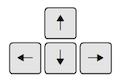
\includegraphics{./img/rstudio_cursorkeys.png}\strut
\end{minipage}\tabularnewline
\bottomrule
\end{longtable}

Take a few minutes to play around at the console and try different
things out. Don't worry if you make a mistake, you can't break anything
easily!

\subsection{Functions}\label{functions}

Functions are a set of instructions that carry out a specific task.
Functions often require some input and generate some output. For
example, instead of using the \texttt{+} operator for addition, we can
use the \texttt{sum} function to add two or more numbers.

\begin{Shaded}
\begin{Highlighting}[]
\KeywordTok{sum}\NormalTok{(}\DecValTok{1}\NormalTok{, }\DecValTok{4}\NormalTok{, }\DecValTok{10}\NormalTok{)}
\end{Highlighting}
\end{Shaded}

\begin{verbatim}
[1] 15
\end{verbatim}

In the example above, \texttt{1,\ 4,\ 10} are the inputs and 15 is the
output. A function always requires the use of parenthesis or round
brackets \texttt{()}. Inputs to the function are called
\textbf{arguments} and go inside the brackets. The output of a function
is displayed on the screen but we can also have the option of saving the
result of the output. More on this later.

\subsection{Getting Help}\label{getting-help}

Another useful function in R is \texttt{help} which we can use to
display online documentation. For example, if we wanted to know how to
use the \texttt{sum} function, we could type \texttt{help(sum)} and look
at the online documentation.

\begin{Shaded}
\begin{Highlighting}[]
\KeywordTok{help}\NormalTok{(sum)}
\end{Highlighting}
\end{Shaded}

The question mark \texttt{?} can also be used as a shortcut to access
online help.

\begin{Shaded}
\begin{Highlighting}[]
\NormalTok{?sum}
\end{Highlighting}
\end{Shaded}

\begin{figure}
\centering
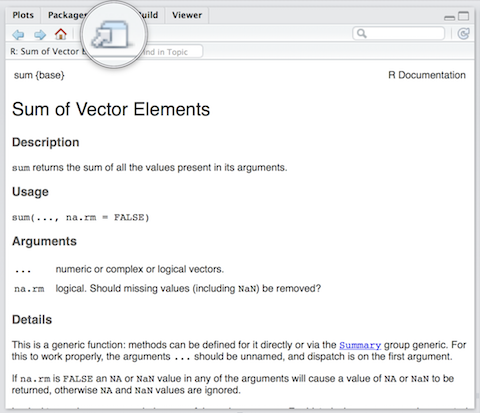
\includegraphics{./img/rstudio_help.png}
\caption{}
\end{figure}

Use the toolbar button shown in the picture above to expand and display
the help in a new window.

Help pages for functions in R follow a consistent layout generally
include these sections:

\begin{longtable}[]{@{}ll@{}}
\toprule
Description & A brief description of the function\tabularnewline
Usage & The complete syntax or grammar including all arguments
(inputs)\tabularnewline
Arguments & Explanation of each argument\tabularnewline
Details & Any relevant details about the function and its
arguments\tabularnewline
Value & The output value of the function\tabularnewline
Examples & Example of how to use the function\tabularnewline
\bottomrule
\end{longtable}

\subsection{The Assignment Operator}\label{the-assignment-operator}

Now we know how to provide inputs to a function using parenthesis or
round brackets \texttt{()}, but what about the output of a function?

We use the assignment operator \textbf{\texttt{\textless{}-}} for
creating or updating objects. If we wanted to save the result of adding
\texttt{sum(1,\ 4,\ 10)}, we would do the following:

\begin{Shaded}
\begin{Highlighting}[]
\NormalTok{myresult <-}\StringTok{ }\KeywordTok{sum}\NormalTok{(}\DecValTok{1}\NormalTok{, }\DecValTok{4}\NormalTok{, }\DecValTok{10}\NormalTok{)}
\end{Highlighting}
\end{Shaded}

The line above creates a new object called \texttt{myresult} in our
environment and saves the result of the \texttt{sum(1,\ 4,\ 10)} in it.
To see what's in \texttt{myresult}, just type it at the console:

\begin{Shaded}
\begin{Highlighting}[]
\NormalTok{myresult}
\end{Highlighting}
\end{Shaded}

\begin{verbatim}
[1] 15
\end{verbatim}

Take a look at the \textbf{Environment} pane in RStudio and you'll see
\texttt{myresult} there.

\begin{figure}
\centering
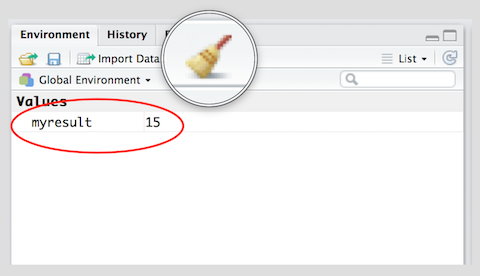
\includegraphics{./img/rstudio_env.png}
\caption{}
\end{figure}

To delete all objects from the environment, you can use the
\textbf{broom} button as shown in the picture above.

We called our object \texttt{myresult} but we can call it anything as
long as we follow a few simple rules. Object names can contain upper or
lower case letters (\texttt{A-Z}, \texttt{a-z}), numbers (\texttt{0-9}),
underscores (\texttt{\_}) or a dot (\texttt{.}) but all object names
must start with a letter. Choose names that are descriptive and easy to
type.

\begin{longtable}[]{@{}ll@{}}
\toprule
Good Object Names & Bad Object Names\tabularnewline
\midrule
\endhead
result & a\tabularnewline
myresult & x1\tabularnewline
my.result & this.name.is.just.too.long\tabularnewline
my\_result &\tabularnewline
data1 &\tabularnewline
\bottomrule
\end{longtable}

\subsection{Sequences}\label{sequences}

We often need to create sequences when manipulating data. For instance,
you might want to perform an operation on the first 10 rows of a dataset
so we need a way to select the range we're interested in.

There are two ways to create a sequence. Let's try to create a sequence
of numbers from 1 to 10 using the two methods:

\begin{enumerate}
\def\labelenumi{\arabic{enumi}.}
\tightlist
\item
  Using the colon \texttt{:} operator. If you're familiar with
  spreadsheets then you might've already used \texttt{:} to select
  cells, for example \texttt{A1:A20}. In R, you can use the \texttt{:}
  to create a sequence in a similar fashion:
\end{enumerate}

\begin{Shaded}
\begin{Highlighting}[]
\DecValTok{1}\OperatorTok{:}\DecValTok{10}
\end{Highlighting}
\end{Shaded}

\begin{verbatim}
 [1]  1  2  3  4  5  6  7  8  9 10
\end{verbatim}

\begin{enumerate}
\def\labelenumi{\arabic{enumi}.}
\tightlist
\item
  Using the \texttt{seq} function we get the exact same result:
\end{enumerate}

\begin{Shaded}
\begin{Highlighting}[]
\KeywordTok{seq}\NormalTok{(}\DataTypeTok{from =} \DecValTok{1}\NormalTok{, }\DataTypeTok{to =} \DecValTok{10}\NormalTok{)}
\end{Highlighting}
\end{Shaded}

\begin{verbatim}
 [1]  1  2  3  4  5  6  7  8  9 10
\end{verbatim}

The \texttt{seq} function has a number of options which control how the
sequence is generated. For example to create a sequence from 0 to 100 in
increments of \texttt{5}, we can use the optional \texttt{by} argument.
Notice how we wrote \texttt{by\ =\ 5} as the third argument. It is a
common practice to specify the name of argument when the argument is
optional. The arguments \texttt{from} and \texttt{to} are not optional,
se we can write \texttt{seq(0,\ 100,\ by\ =\ 5)} instead of
\texttt{seq(from\ =\ 0,\ to\ =\ 100,\ by\ =\ 5)}. Both, are valid ways
of achieving the same outcome. You can code whichever way you like. We
recommend to write code such that you make it easy for your future self
and others to read and understand the code.

\begin{Shaded}
\begin{Highlighting}[]
\KeywordTok{seq}\NormalTok{(}\DataTypeTok{from =} \DecValTok{0}\NormalTok{, }\DataTypeTok{to =} \DecValTok{100}\NormalTok{, }\DataTypeTok{by =} \DecValTok{5}\NormalTok{)}
\end{Highlighting}
\end{Shaded}

\begin{verbatim}
 [1]   0   5  10  15  20  25  30  35  40  45  50  55  60  65  70  75  80
[18]  85  90  95 100
\end{verbatim}

Another common use of the \texttt{seq} function is to create a sequence
of a specific length. Here, we create a sequence from 0 to 100 with
length 9, i.e., the result is a vector with 9 elements.

\begin{Shaded}
\begin{Highlighting}[]
\KeywordTok{seq}\NormalTok{(}\DataTypeTok{from =} \DecValTok{0}\NormalTok{, }\DataTypeTok{to =} \DecValTok{100}\NormalTok{, }\DataTypeTok{length.out =}  \DecValTok{9}\NormalTok{)}
\end{Highlighting}
\end{Shaded}

\begin{verbatim}
[1]   0.0  12.5  25.0  37.5  50.0  62.5  75.0  87.5 100.0
\end{verbatim}

Now it's your turn:

\begin{itemize}
\tightlist
\item
  Create a sequence of \textbf{odd} numbers between 0 and 100 and save
  it in an object called \texttt{odd\_numbers}
\end{itemize}

\begin{Shaded}
\begin{Highlighting}[]
\NormalTok{odd_numbers <-}\StringTok{ }\KeywordTok{seq}\NormalTok{(}\DecValTok{1}\NormalTok{, }\DecValTok{100}\NormalTok{, }\DecValTok{2}\NormalTok{)}
\end{Highlighting}
\end{Shaded}

\begin{itemize}
\tightlist
\item
  Next, display \texttt{odd\_numbers} on the console to verify that you
  did it correctly
\end{itemize}

\begin{Shaded}
\begin{Highlighting}[]
\NormalTok{odd_numbers}
\end{Highlighting}
\end{Shaded}

\begin{verbatim}
 [1]  1  3  5  7  9 11 13 15 17 19 21 23 25 27 29 31 33 35 37 39 41 43 45
[24] 47 49 51 53 55 57 59 61 63 65 67 69 71 73 75 77 79 81 83 85 87 89 91
[47] 93 95 97 99
\end{verbatim}

\begin{itemize}
\item
  What do the numbers in square brackets \texttt{{[}\ {]}} mean? Look at
  the number of values displayed in each line to find out the answer.
\item
  Use the \texttt{length} function to find out how many values are in
  the object \texttt{odd\_numbers}.

  \begin{itemize}
  \tightlist
  \item
    HINT: Try \texttt{help(length)} and look at the examples section at
    the end of the help screen.
  \end{itemize}
\end{itemize}

\begin{Shaded}
\begin{Highlighting}[]
\KeywordTok{length}\NormalTok{(odd_numbers)}
\end{Highlighting}
\end{Shaded}

\begin{verbatim}
[1] 50
\end{verbatim}

\subsection{Scripts}\label{scripts}

The Console is great for simple tasks but if you're working on a project
you would mostly likely want to save your work in some sort of a
document or a file. Scripts in R are just plain text files that contain
R code. You can edit a script just like you would edit a file in any
word processing or note-taking application.

Create a new script using the menu or the toolbar button as shown below.

\begin{figure}
\centering
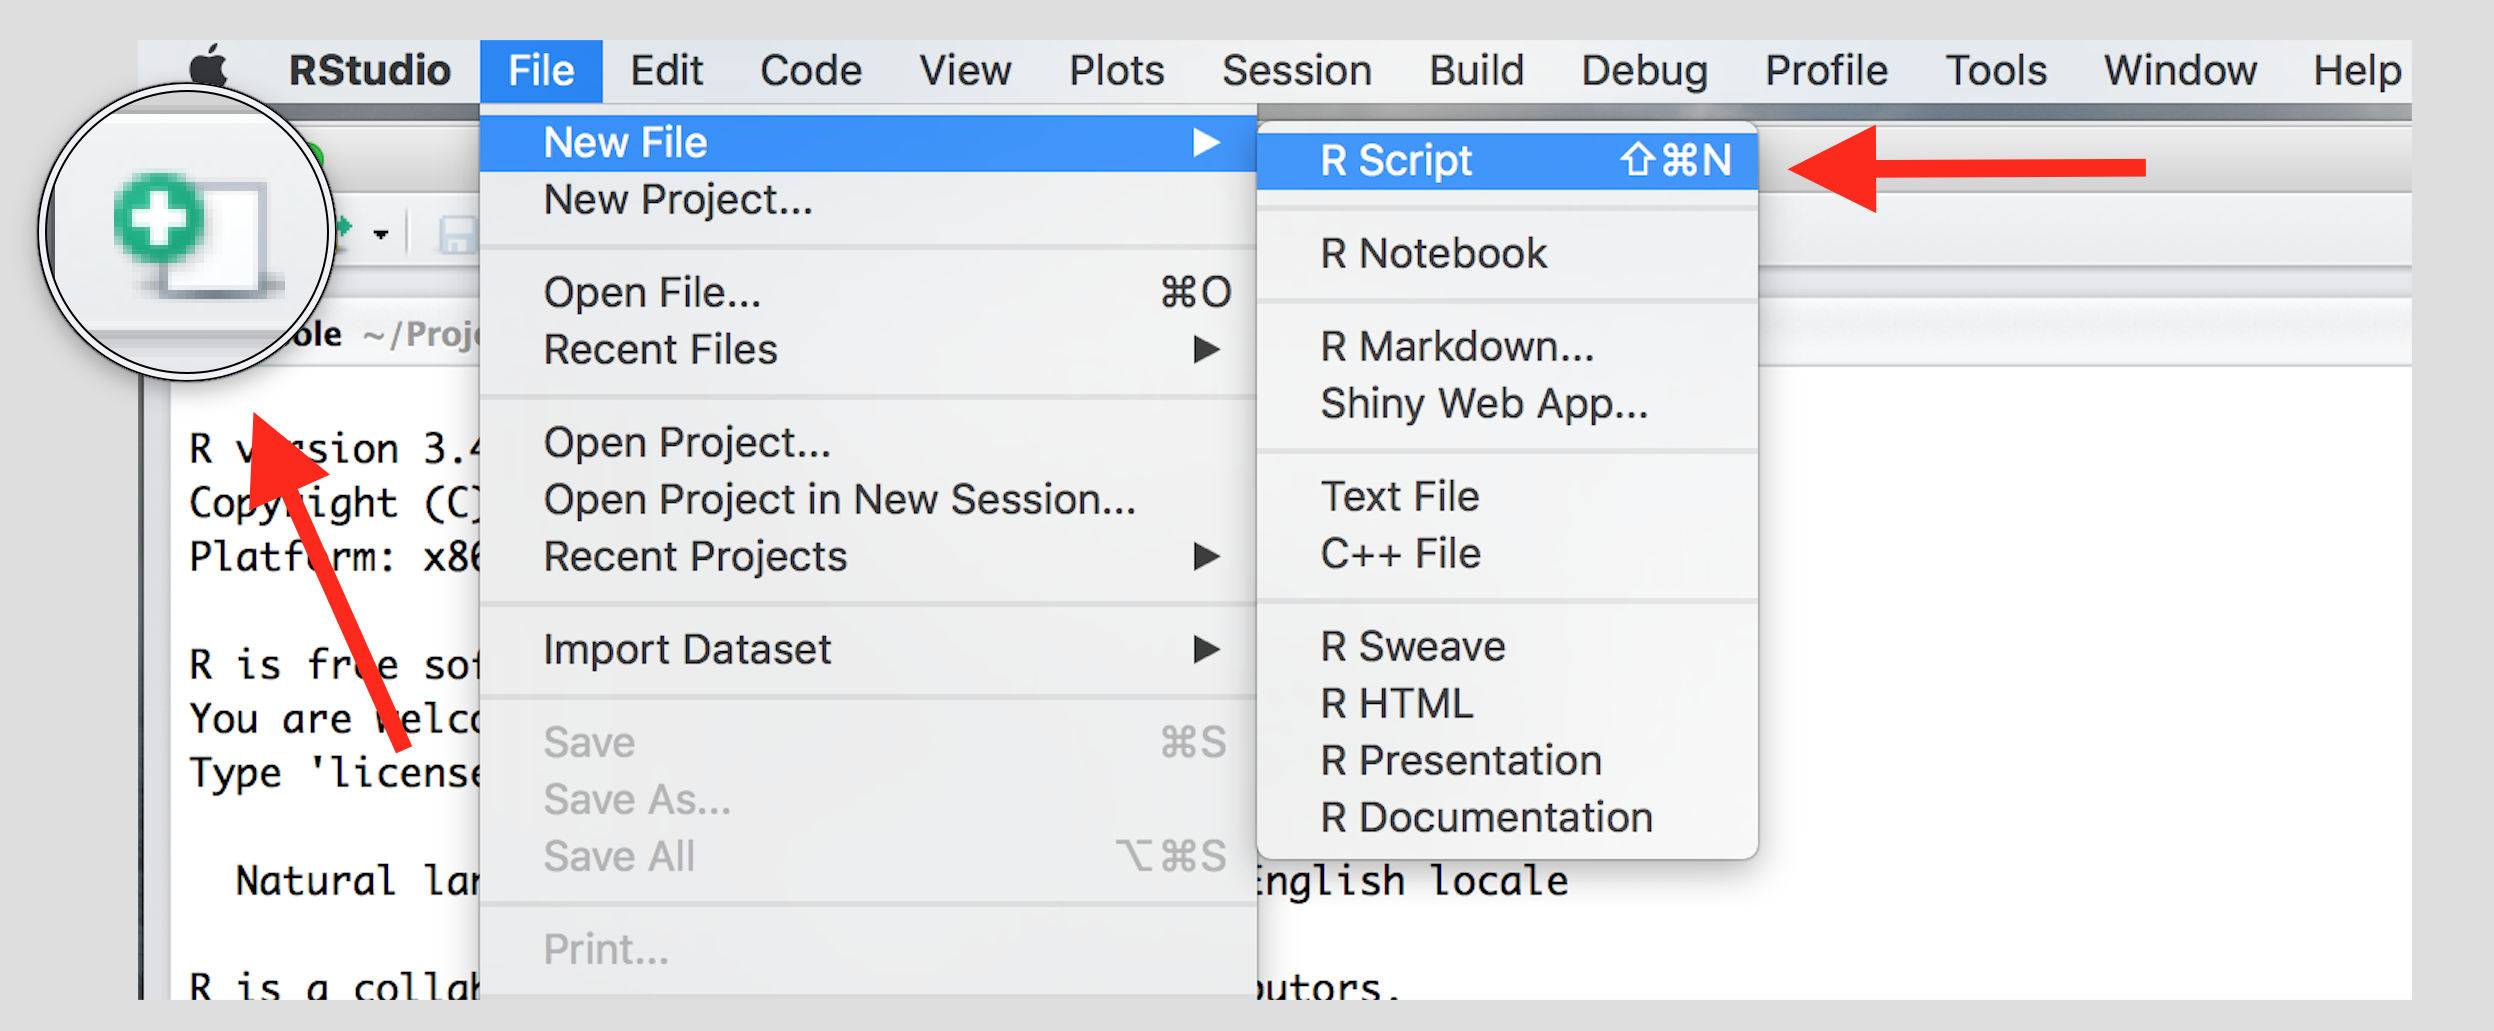
\includegraphics{./img/rstudio_newfile.png}
\caption{}
\end{figure}

Once you've created a script, it is generally a good idea to give it a
meaningful name and save it immediately. For our first session save your
script as \textbf{seminar1.R}

\begin{longtable}[]{@{}ll@{}}
\toprule
\begin{minipage}[t]{0.52\columnwidth}\raggedright\strut
Familiarize yourself with the script window in RStudio, and especially
the two buttons labeled \textbf{Run} and \textbf{Source}\strut
\end{minipage} & \begin{minipage}[t]{0.42\columnwidth}\raggedright\strut
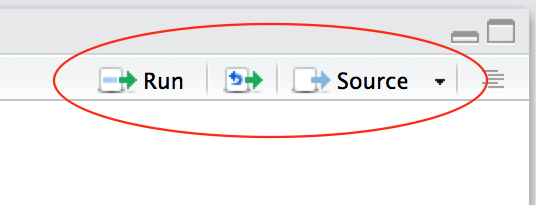
\includegraphics{./img/rstudio_script.png}\strut
\end{minipage}\tabularnewline
\bottomrule
\end{longtable}

There are a few different ways to run your code from a script.

\begin{longtable}[]{@{}ll@{}}
\toprule
\begin{minipage}[t]{0.24\columnwidth}\raggedright\strut
One line at a time\strut
\end{minipage} & \begin{minipage}[t]{0.70\columnwidth}\raggedright\strut
Place the cursor on the line you want to run and hit CTRL-ENTER or use
the \textbf{Run} button\strut
\end{minipage}\tabularnewline
\begin{minipage}[t]{0.24\columnwidth}\raggedright\strut
Multiple lines\strut
\end{minipage} & \begin{minipage}[t]{0.70\columnwidth}\raggedright\strut
Select the lines you want to run and hit CTRL-ENTER or use the
\textbf{Run} button\strut
\end{minipage}\tabularnewline
\begin{minipage}[t]{0.24\columnwidth}\raggedright\strut
Entire script\strut
\end{minipage} & \begin{minipage}[t]{0.70\columnwidth}\raggedright\strut
Use the \textbf{Source} button\strut
\end{minipage}\tabularnewline
\bottomrule
\end{longtable}

\subsection{Central Tendency}\label{central-tendency}

The appropriate measure of central tendency depends on the level of
measurement of the variable. To recap:

\begin{longtable}[]{@{}ll@{}}
\toprule
Level of measurement & Appropriate measure of central
tendency\tabularnewline
\midrule
\endhead
Continuous & arithmetic mean (or average)\tabularnewline
Ordered & median (or the central observation)\tabularnewline
Nominal & mode (the most frequent value)\tabularnewline
\bottomrule
\end{longtable}

\subsubsection{Mean}\label{mean}

We calculate the average grade on our eleven homework assignments in
statistics 1. We create our vector of 11 (fake) grades first using the
\texttt{c()} function, where \texttt{c} stands for collect or
concatenate.

\begin{Shaded}
\begin{Highlighting}[]
\NormalTok{hw.grades <-}\StringTok{ }\KeywordTok{c}\NormalTok{(}\DecValTok{80}\NormalTok{, }\DecValTok{90}\NormalTok{, }\DecValTok{85}\NormalTok{, }\DecValTok{71}\NormalTok{, }\DecValTok{69}\NormalTok{, }\DecValTok{85}\NormalTok{, }\DecValTok{83}\NormalTok{, }\DecValTok{88}\NormalTok{, }\DecValTok{99}\NormalTok{, }\DecValTok{81}\NormalTok{, }\DecValTok{92}\NormalTok{)}
\end{Highlighting}
\end{Shaded}

We now take the sum of the grades.

\begin{Shaded}
\begin{Highlighting}[]
\NormalTok{sum.hw.grades <-}\StringTok{ }\KeywordTok{sum}\NormalTok{(hw.grades)}
\end{Highlighting}
\end{Shaded}

We also take the number of grades

\begin{Shaded}
\begin{Highlighting}[]
\NormalTok{number.hw.grades <-}\StringTok{ }\KeywordTok{length}\NormalTok{(hw.grades) }
\end{Highlighting}
\end{Shaded}

The mean is the sum of grades over the number of grades.

\begin{Shaded}
\begin{Highlighting}[]
\NormalTok{sum.hw.grades }\OperatorTok{/}\StringTok{ }\NormalTok{number.hw.grades}
\end{Highlighting}
\end{Shaded}

\begin{verbatim}
[1] 83.90909
\end{verbatim}

R provides us with an even easier way to do the same with a function
called \href{http://bit.ly/R_mean}{\texttt{mean()}}.

\begin{Shaded}
\begin{Highlighting}[]
\KeywordTok{mean}\NormalTok{(hw.grades)}
\end{Highlighting}
\end{Shaded}

\begin{verbatim}
[1] 83.90909
\end{verbatim}

\subsubsection{Median}\label{median}

The median is the appropriate measure of central tendency for ordinal
variables. Ordinal means that there is a rank ordering but not equally
spaced intervals between values of the variable. Education is a common
example. In education, more education is better. But the difference
between primary school and secondary school is not the same as the
difference between secondary school and an undergraduate degree.

Let's generate a fake example with 100 people. We use numbers to code
different levels of education.

\begin{longtable}[]{@{}lll@{}}
\toprule
Code & Meaning & Frequency in our data\tabularnewline
0 & no education & 1\tabularnewline
1 & primary school & 5\tabularnewline
2 & secondary school & 55\tabularnewline
3 & undergraduate degree & 20\tabularnewline
4 & postgraduate degree & 10\tabularnewline
5 & doctorate & 9\tabularnewline
\bottomrule
\end{longtable}

We introduce a new function to create a vector. The function
\texttt{rep()}, replicates elements of a vector. Its arguments are the
item \texttt{x} to be replicated and the number of \texttt{times} to
replicate. Below, we create the variable education with the frequency of
education level indicated above. Note that the arguments \texttt{x} and
\texttt{times} do not have to be written out.

\begin{Shaded}
\begin{Highlighting}[]
\NormalTok{edu <-}\StringTok{ }\KeywordTok{c}\NormalTok{( }\KeywordTok{rep}\NormalTok{(}\DataTypeTok{x=}\DecValTok{0}\NormalTok{, }\DataTypeTok{times=}\DecValTok{1}\NormalTok{), }\KeywordTok{rep}\NormalTok{(}\DataTypeTok{x=}\DecValTok{1}\NormalTok{, }\DataTypeTok{times=}\DecValTok{5}\NormalTok{), }\KeywordTok{rep}\NormalTok{(}\DataTypeTok{x=}\DecValTok{2}\NormalTok{, }\DataTypeTok{times=}\DecValTok{55}\NormalTok{),}
          \KeywordTok{rep}\NormalTok{(}\DataTypeTok{x=}\DecValTok{3}\NormalTok{, }\DataTypeTok{times=}\DecValTok{20}\NormalTok{), }\KeywordTok{rep}\NormalTok{(}\DecValTok{4}\NormalTok{,}\DecValTok{10}\NormalTok{), }\KeywordTok{rep}\NormalTok{(}\DecValTok{5}\NormalTok{,}\DecValTok{9}\NormalTok{) )}
\end{Highlighting}
\end{Shaded}

The median level of education is the level where 50 percent of the
observations have a lower or equal level of education and 50 percent
have a higher or equal level of education. That means that the median
splits the data in half.

We use the \href{http://bit.ly/R_median}{\texttt{median()}} function for
finding the median.

\begin{Shaded}
\begin{Highlighting}[]
\KeywordTok{median}\NormalTok{(edu)}
\end{Highlighting}
\end{Shaded}

\begin{verbatim}
[1] 2
\end{verbatim}

The median level of education is secondary school.

\subsubsection{Mode}\label{mode}

The mode is the appropriate measure of central tendency if the level of
measurement is nominal. Nominal means that there is no ordering implicit
in the values that a variable takes on. We create data from 1000 (fake)
voters in the United Kingdom who each express their preference on
remaining in or leaving the European Union. The options are leave or
stay. Leaving is not greater than staying and vice versa (even though we
all order the two options normatively).

\begin{longtable}[]{@{}lll@{}}
\toprule
Code & Meaning & Frequency in our data\tabularnewline
0 & leave & 509\tabularnewline
1 & stay & 491\tabularnewline
\bottomrule
\end{longtable}

\begin{Shaded}
\begin{Highlighting}[]
\NormalTok{stay <-}\StringTok{ }\KeywordTok{c}\NormalTok{(}\KeywordTok{rep}\NormalTok{(}\DecValTok{0}\NormalTok{, }\DecValTok{509}\NormalTok{), }\KeywordTok{rep}\NormalTok{(}\DecValTok{1}\NormalTok{, }\DecValTok{491}\NormalTok{))}
\end{Highlighting}
\end{Shaded}

The mode is the most common value in the data. There is no mode function
in R. The most straightforward way to determine the mode is to use the
\href{http://bit.ly/R_table}{\texttt{table()}} function. It returns a
frequency table. We can easily see the mode in the table. As your coding
skills increase, you will see other ways of recovering the mode from a
vector.

\begin{Shaded}
\begin{Highlighting}[]
\KeywordTok{table}\NormalTok{(stay)}
\end{Highlighting}
\end{Shaded}

\begin{verbatim}
stay
  0   1 
509 491 
\end{verbatim}

The mode is leaving the EU because the number of `leavers' (0) is
greater than the number of `remainers' (1).

\subsection{Dispersion}\label{dispersion}

The appropriate measure of dispersion depends on the level of
measurement of the variable we wish to describe.

\begin{longtable}[]{@{}ll@{}}
\toprule
Level of measurement & Appropriate measure of dispersion\tabularnewline
\midrule
\endhead
Continuous & variance and/or standard deviation\tabularnewline
Ordered & range or interquartile range\tabularnewline
Nominal & proportion in each category\tabularnewline
\bottomrule
\end{longtable}

\subsubsection{Variance and standard
deviation}\label{variance-and-standard-deviation}

Both the variance and the standard deviation tell by how much an average
realisation of a variable differs from the mean of that variable. Let's
assume that our variable is income in the UK. Let's assume that its mean
is 35 000 per year. We also assume that the average deviation from 35
000 is 5 000. If we ask 100 people in the UK at random about their
income, we get 100 different answers. If we average the differences
betweeen the 100 answers and 35 000, we would get 5 000. Suppose that
the average income in France is also 35 000 per year but the average
deviation is 10 000 instead. This would imply that income is more
equally distributed in the UK than in France.

Dispersion is important to describe data as this example illustrates.
Although, mean income in our hypothetical example is the same in France
and the UK, the distribution is tighter in the UK. The figure below
illustrates our example:

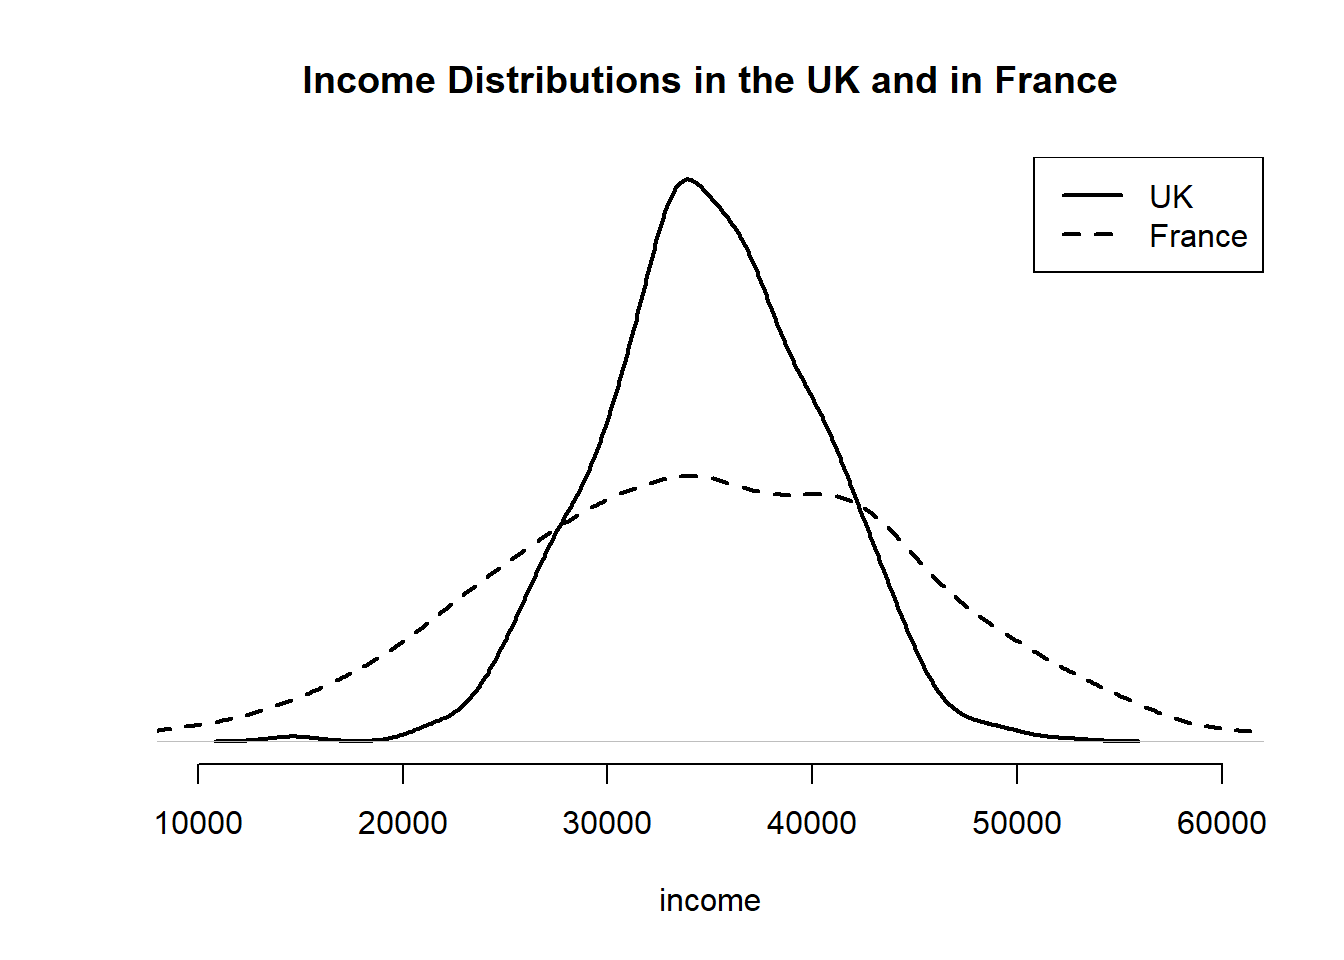
\includegraphics{statistics1_files/figure-latex/unnamed-chunk-26-1.pdf}

The variance gives us an idea about the variability of data. The formula
for the variance in the population is
\[ \frac{\sum_{i=1}^n(x_i - \mu_x)^2}{n}\]

The formula for the variance in a sample adjusts for sampling
variability, i.e., uncertainty about how well our sample reflects the
population by subtracting 1 in the denominator. Subtracting 1 will have
next to no effect if n is large but the effect increases the smaller n.
The smaller n, the larger the sample variance. The intuition is, that in
smaller samples, we are less certain that our sample reflects the
population. We, therefore, adjust variability of the data upwards. The
formula is

\[ \frac{\sum_{i=1}^n(x_i - \bar{x})^2}{n-1}\]

Notice the different notation for the mean in the two formulas. We write
\(\mu_x\) for the mean of x in the population and \(\bar{x}\) for the
mean of x in the sample. Notation is, however, unfortunately not always
consistent.

Take a minute to think your way through the formula. There are 4 setps:
(1), In the numerator, we subtract the mean of x from some realisation
of x. (2), We square the deviations from the mean because we want
positive numbers only. (3) We sum the squared deviations. (4) We divide
the sum by \((n-1)\). Below we show this for the homework example. In
the last row, we add a 5th step. We take the square root in order to
return to the orginial units of the homework grades.

\begin{longtable}[]{@{}llll@{}}
\toprule
Obs & Var & Dev. from mean & Squared dev. from mean\tabularnewline
\midrule
\endhead
i & grade & \(x_i-\bar{x}\) & \((x_i-\bar{x})^2\)\tabularnewline
1 & 80 & -3.9090909 & 15.2809917\tabularnewline
2 & 90 & 6.0909091 & 37.0991736\tabularnewline
3 & 85 & 1.0909091 & 1.1900826\tabularnewline
4 & 71 & -12.9090909 & 166.6446281\tabularnewline
5 & 69 & -14.9090909 & 222.2809917\tabularnewline
6 & 85 & 1.0909091 & 1.1900826\tabularnewline
7 & 83 & -0.9090909 & 0.8264463\tabularnewline
8 & 88 & 4.0909091 & 16.7355372\tabularnewline
9 & 99 & 15.0909091 & 227.7355372\tabularnewline
10 & 81 & -2.9090909 & 8.4628099\tabularnewline
11 & 92 & 8.0909091 & 65.4628099\tabularnewline
\(\sum_{i=1}^n\) & & & 762.9090909\tabularnewline
\(\div n-1\) & & & 76.2909091\tabularnewline
\(\sqrt{}\) & & & 8.7344667\tabularnewline
\bottomrule
\end{longtable}

Our first grade (80) is below the mean (83.9090909). The sum is, thus,
negative. Our second grade (90) is above the mean, so that the sum is
positive. Both are deviations from the mean (think of them as
distances). Our sum shall reflect the total sum of distances and
distances must be positive. Hence, we square the distances from the
mean. Having done this for all eleven observations, we sum the squared
distances. Dividing by 10 (with the sample adjustment), gives us the
average squared deviation. This is the variance. The units of the
variance---squared deviations---are somewhat awkward. We return to this
in a moment.

We take the variance in R by using the
\href{http://bit.ly/R_var}{\texttt{var()}} function. By default
\texttt{var()} takes the sample variance.

\begin{Shaded}
\begin{Highlighting}[]
\KeywordTok{var}\NormalTok{(hw.grades)}
\end{Highlighting}
\end{Shaded}

\begin{verbatim}
[1] 76.29091
\end{verbatim}

The average squared difference form our mean grade is 76.2909091. But
what does that mean? We would like to get rid of the square in our
units. That's what the standard deviation does. The standard deviation
is the square root over the variance.

\[ \sqrt{\frac{\sum_{i=1}^n(x_i - \bar{x})^2}{n-1}}\]

We get the average deviation from our mean grade (83.9090909) with the
\href{http://bit.ly/R_sd}{\texttt{sd()}} function.

\begin{Shaded}
\begin{Highlighting}[]
\KeywordTok{sd}\NormalTok{(hw.grades)}
\end{Highlighting}
\end{Shaded}

\begin{verbatim}
[1] 8.734467
\end{verbatim}

The standard deviation is much more intuitive than the variance because
its units are the same as the units of the variable we are interested
in. ``Why teach us about this awful variance then'', you ask.
Mathematically, we have to compute the variance before getting the
standard deviation. We recommend that you use the standard deviation to
describe the variability of your continuous data.

Note: We used the sample variance and sample standard deviation
formulas. If the eleven assignments represent the population, we would
use the population variance formula. Whether the 11 cases represent a
sample or the population depends on what we want to know. If we want
learn about all students' assignments or future assignments, the 11
cases are a sample.

\subsubsection{Range and interquartile
range}\label{range-and-interquartile-range}

The proper measure of dispersion of an ordinal variable is the range or
the interquartile range. The interquartile range is usually the
preferred measure because the range is strongly affected by outlying
cases.

Let's take the range first. We get back to our education example. In R,
we use the \href{http://bit.ly/R_range}{\texttt{range()}} function to
compute the range.

\begin{Shaded}
\begin{Highlighting}[]
\KeywordTok{range}\NormalTok{(edu)}
\end{Highlighting}
\end{Shaded}

\begin{verbatim}
[1] 0 5
\end{verbatim}

Our data ranges from no education all the way to those with a doctorate.
However, no education is not a common value. Only one person in our
sample did not have any education. The interquartile range is the range
from the 25th to the 75th percentiles, i.e., it contains the central 50
percent of the distribution.

The 25th percentile is the value of education that 25 percent or fewer
people have (when we order education from lowest to highest). We use the
\href{http://bit.ly/R_quantile}{\texttt{quantile()}} function in R to
get percentiles. The function takes two arguments: \texttt{x} is the
data vector and \texttt{probs} is the percentile.

\begin{Shaded}
\begin{Highlighting}[]
\KeywordTok{quantile}\NormalTok{(edu, }\FloatTok{0.25}\NormalTok{) }\CommentTok{# 25th percentile}
\end{Highlighting}
\end{Shaded}

\begin{verbatim}
25% 
  2 
\end{verbatim}

\begin{Shaded}
\begin{Highlighting}[]
\KeywordTok{quantile}\NormalTok{(edu, }\FloatTok{0.75}\NormalTok{) }\CommentTok{# 75th percentile}
\end{Highlighting}
\end{Shaded}

\begin{verbatim}
75% 
  3 
\end{verbatim}

Therefore, the interquartile range is from 2, secondary school to 3,
undergraduate degree.

\subsubsection{Proportion in each
category}\label{proportion-in-each-category}

To describe the distribution of our nominal variable, support for
remaining in the European Union, we use the proportions in each
category.

Recall, that we looked at the frequency table to determine the mode:

\begin{Shaded}
\begin{Highlighting}[]
\KeywordTok{table}\NormalTok{(stay)}
\end{Highlighting}
\end{Shaded}

\begin{verbatim}
stay
  0   1 
509 491 
\end{verbatim}

To get the proportions in each category, we divide the values in the
table, i.e., 509 and 491, by the sum of the table, i.e., 1000.

\begin{Shaded}
\begin{Highlighting}[]
\KeywordTok{table}\NormalTok{(stay) }\OperatorTok{/}\StringTok{ }\KeywordTok{sum}\NormalTok{(}\KeywordTok{table}\NormalTok{(stay))}
\end{Highlighting}
\end{Shaded}

\begin{verbatim}
stay
    0     1 
0.509 0.491 
\end{verbatim}

\subsection{Exercises}\label{exercises}

\begin{enumerate}
\def\labelenumi{\arabic{enumi}.}
\tightlist
\item
  Create a script and call it assignment01. Save your script.
\item
  Download this
  \href{https://www.rstudio.com/wp-content/uploads/2016/06/r-cheat-sheet.pdf}{cheat-sheet}
  and go over it. You won't understand most of it right a away. But it
  will become a useful resource. Look at it often.
\item
  Calculate the square root of 1369 using the \texttt{sqrt()} function.
\item
  Square the number 13 using the \texttt{\^{}} operator.
\item
  What is the result of summing all numbers from 1 to 100?
\end{enumerate}

We take a sample of yearly income in Berlin. The values that we got are:
19395, 22698, 40587, 25705, 26292, 42150, 29609, 12349, 18131, 20543,
37240, 28598, 29007, 26106, 19441, 42869, 29978, 5333, 32013, 20272,
14321, 22820, 14739, 17711, 18749.

\begin{enumerate}
\def\labelenumi{\arabic{enumi}.}
\setcounter{enumi}{5}
\tightlist
\item
  Create the variable \texttt{income} with the values form our Berlin
  sample in R.
\item
  Describe Berlin income using the appropriate measures of central
  tendency and dispersion.
\item
  Compute the average deviation without using the \texttt{sd()}
  function.
\end{enumerate}

Take a look at the Sunday Question (who would you vote for if the
general election were next Sunday?) by following this link
\href{https://www.wahlrecht.de/umfragen/}{Sunday Question Germany}. You
should be able to translate the website into English by right clicking
in your browser and clicking ``Translate to English.''

\begin{enumerate}
\def\labelenumi{\arabic{enumi}.}
\setcounter{enumi}{8}
\tightlist
\item
  What is the level of measurement of the variable in the Sunday
  Question?
\item
  Take the most recent poll and describe what you see in terms of
  central tendency and dispersion.
\item
  Save your script, which should now include the answers to all the
  exercises.
\item
  Source your script, i.e.~run the entire script without error message.
  Clean your script if you get error messages.
\end{enumerate}

\section{Solutions}\label{solutions}

\subsection{Exercise 3}\label{exercise-3}

Calculate the square root of 1369 using the \texttt{sqrt()} function.

\begin{Shaded}
\begin{Highlighting}[]
\KeywordTok{sqrt}\NormalTok{(}\DecValTok{1369}\NormalTok{)}
\end{Highlighting}
\end{Shaded}

\begin{verbatim}
[1] 37
\end{verbatim}

\subsection{Exercise 4}\label{exercise-4}

Square the number 13 using the \texttt{\^{}} operator.

\begin{Shaded}
\begin{Highlighting}[]
\DecValTok{13}\OperatorTok{^}\DecValTok{2}
\end{Highlighting}
\end{Shaded}

\begin{verbatim}
[1] 169
\end{verbatim}

\subsection{Exercise 5}\label{exercise-5}

What is the result of summing all numbers from 1 to 100?

\begin{Shaded}
\begin{Highlighting}[]
\CommentTok{# sequence of numbers from 1 to 100 in steps of 1}
\NormalTok{numbers_1_to_}\DecValTok{100}\NormalTok{ <-}\StringTok{ }\KeywordTok{seq}\NormalTok{(}\DataTypeTok{from =} \DecValTok{1}\NormalTok{, }\DataTypeTok{to =} \DecValTok{100}\NormalTok{, }\DataTypeTok{by =} \DecValTok{1}\NormalTok{)}
\CommentTok{# sum over the vector}
\NormalTok{result <-}\StringTok{ }\KeywordTok{sum}\NormalTok{(numbers_1_to_}\DecValTok{100}\NormalTok{)}
\CommentTok{# print the result}
\NormalTok{result}
\end{Highlighting}
\end{Shaded}

\begin{verbatim}
[1] 5050
\end{verbatim}

The result is 5050.

\subsection{Exercise 6}\label{exercise-6}

Create the variable \emph{income} with the values form our Berlin sample
in R.

\begin{Shaded}
\begin{Highlighting}[]
\CommentTok{# create the income variable using the c() function}
\NormalTok{income <-}\StringTok{ }\KeywordTok{c}\NormalTok{(}
  \DecValTok{19395}\NormalTok{, }\DecValTok{22698}\NormalTok{, }\DecValTok{40587}\NormalTok{, }\DecValTok{25705}\NormalTok{, }\DecValTok{26292}\NormalTok{, }\DecValTok{42150}\NormalTok{, }\DecValTok{29609}\NormalTok{, }\DecValTok{12349}\NormalTok{, }\DecValTok{18131}\NormalTok{, }
  \DecValTok{20543}\NormalTok{, }\DecValTok{37240}\NormalTok{, }\DecValTok{28598}\NormalTok{, }\DecValTok{29007}\NormalTok{, }\DecValTok{26106}\NormalTok{, }\DecValTok{19441}\NormalTok{, }\DecValTok{42869}\NormalTok{, }\DecValTok{29978}\NormalTok{, }\DecValTok{5333}\NormalTok{, }
  \DecValTok{32013}\NormalTok{, }\DecValTok{20272}\NormalTok{, }\DecValTok{14321}\NormalTok{, }\DecValTok{22820}\NormalTok{, }\DecValTok{14739}\NormalTok{, }\DecValTok{17711}\NormalTok{, }\DecValTok{18749}
\NormalTok{)}
\end{Highlighting}
\end{Shaded}

\subsection{Exercise 7}\label{exercise-7}

Describe Berlin income using the appropriate measures of central
tendency and dispersion.

We use the mean for the central tendency of \emph{income}. The variable
is interval scaled and the mean is the appropriate measure of central
tendency for interval scaled variables. Our \emph{income} variable is
also normally distributed. Income distributions in most countries are
right skewed. Therefore, the central tendency of income is often
described using the median.

When asked, e.g., in an exam, to describe the central tendency of an
interval scaled variable, use the mean. You can also use the median if
you tell us why.

\begin{Shaded}
\begin{Highlighting}[]
\CommentTok{# central tendency of income}
\KeywordTok{mean}\NormalTok{(income)}
\end{Highlighting}
\end{Shaded}

\begin{verbatim}
[1] 24666.24
\end{verbatim}

\begin{Shaded}
\begin{Highlighting}[]
\CommentTok{# dispersion}
\KeywordTok{sd}\NormalTok{(income)}
\end{Highlighting}
\end{Shaded}

\begin{verbatim}
[1] 9467.383
\end{verbatim}

Average income in our Berlin sample is 24666.24. The average difference
from that value is 9467.38.

\subsection{Exercise 8}\label{exercise-8}

Compute the average deviation without using the sd() function.

We do this in several steps. First, we compute the mean.

\begin{Shaded}
\begin{Highlighting}[]
\NormalTok{mean.income <-}\StringTok{ }\KeywordTok{sum}\NormalTok{(income) }\OperatorTok{/}\StringTok{ }\KeywordTok{length}\NormalTok{(income)}

\CommentTok{# let's print the mean}
\NormalTok{mean.income}
\end{Highlighting}
\end{Shaded}

\begin{verbatim}
[1] 24666.24
\end{verbatim}

Second, we take the differences between each individual realisation of
income and the mean of \emph{income}. The result must be a vector with
the same amount of elements as the \emph{income} vector.

\begin{Shaded}
\begin{Highlighting}[]
\CommentTok{# individual differences between each realisation of income and the mean of income}
\NormalTok{diffs.from.mean <-}\StringTok{ }\NormalTok{income }\OperatorTok{-}\StringTok{ }\NormalTok{mean.income}

\CommentTok{# let's print the vector of differences}
\NormalTok{diffs.from.mean}
\end{Highlighting}
\end{Shaded}

\begin{verbatim}
 [1]  -5271.24  -1968.24  15920.76   1038.76   1625.76  17483.76   4942.76
 [8] -12317.24  -6535.24  -4123.24  12573.76   3931.76   4340.76   1439.76
[15]  -5225.24  18202.76   5311.76 -19333.24   7346.76  -4394.24 -10345.24
[22]  -1846.24  -9927.24  -6955.24  -5917.24
\end{verbatim}

You may be surprised that this works. After all, \emph{income} is a
vector with 25 elements and \emph{mean.income} is a scalar (only one
value). R treats all variables as vectors. It notices that
\emph{mean.income} is a shorter vector than \emph{income}. The former
has 1 element and the latter 25. The vector \emph{mean.income} is
recycled, so that it has the same length as \emph{income} where each
element is the same: the mean of \emph{income}. If you did not
understand this don't worry. The important thing is that it works.

Our next step is to square the differences from the mean.

\begin{Shaded}
\begin{Highlighting}[]
\CommentTok{# square each element in the diffs.from.mean vector}
\NormalTok{squared.diffs.from.mean <-}\StringTok{ }\NormalTok{diffs.from.mean}\OperatorTok{^}\DecValTok{2}

\CommentTok{# print the squared vecto}
\NormalTok{squared.diffs.from.mean}
\end{Highlighting}
\end{Shaded}

\begin{verbatim}
 [1]  27785971   3873969 253470599   1079022   2643096 305681864  24430876
 [8] 151714401  42709362  17001108 158099441  15458737  18842197   2072909
[15]  27303133 331340472  28214794 373774169  53974882  19309345 107023991
[22]   3408602  98550094  48375363  35013729
\end{verbatim}

We squared each individual element in the vector. Therefore, our new
variable \emph{squared.diffs.from.mean} still has 25 elements.

Squaring a value does two things. First, all values in our vector have
become positive. Second, the marginal increase increases with distance,
i.e., values that are close to the mean are only somewhat larger whereas
values that are further from the mean become way larger. To see this,
lets plot the square (we haven't shown you the plot function yet, but we
will do this next seminar).

\begin{Shaded}
\begin{Highlighting}[]
\CommentTok{# a vector of x values from negative 100 to positive 100}
\NormalTok{a <-}\StringTok{ }\KeywordTok{seq}\NormalTok{(}\DataTypeTok{from =} \OperatorTok{-}\DecValTok{100}\NormalTok{, }\DataTypeTok{to =} \DecValTok{100}\NormalTok{, }\DataTypeTok{length.out =} \DecValTok{200}\NormalTok{)}

\CommentTok{# the square of that vector}
\NormalTok{b <-}\StringTok{ }\NormalTok{a}\OperatorTok{^}\DecValTok{2}

\CommentTok{# we plot the input vector a against b, where b is on the y-axis}
\KeywordTok{plot}\NormalTok{(}
  \DataTypeTok{x =}\NormalTok{ a, }\CommentTok{# x-axis values}
  \DataTypeTok{y =}\NormalTok{ b, }\CommentTok{# y-axis values}
  \DataTypeTok{bty =} \StringTok{"n"}\NormalTok{, }\CommentTok{# no border around plot}
  \DataTypeTok{type =} \StringTok{"l"}\NormalTok{, }\CommentTok{# connect individual dots to a line}
  \DataTypeTok{xlab =} \StringTok{"input values from vector a"}\NormalTok{, }\CommentTok{# x axis label}
  \DataTypeTok{ylab =} \StringTok{"b = a^2"} \CommentTok{# y axis label}
\NormalTok{)}
\end{Highlighting}
\end{Shaded}

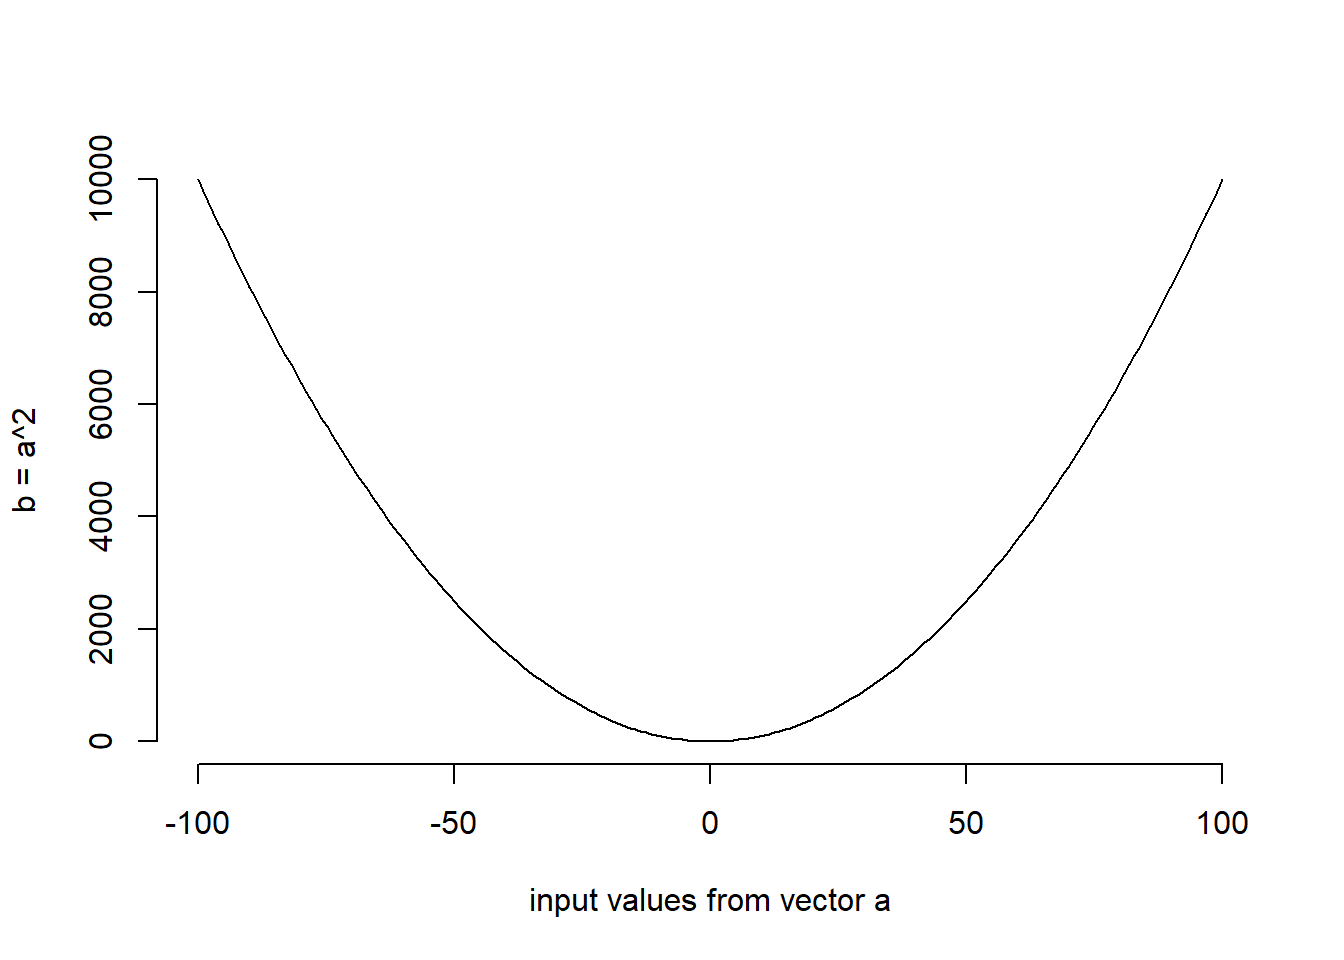
\includegraphics{statistics1_files/figure-latex/unnamed-chunk-43-1.pdf}

In this plot, you should see that the slope of the line increases, the
further we are from 0. We are taking individual differences from the
mean. Hence, if a value is exactly at the mean, the difference is zero.
The further, the value is from the mean (in any direction), the larger
the output value.

We will sum over the individual elements in the next step. Hence, values
that are further from the mean have a larger impact on the sum than
values that are closer to the mean.

In the next step, we take the sum over our squared deviations from the
mean

\begin{Shaded}
\begin{Highlighting}[]
\CommentTok{# sum over squared deviations vector}
\NormalTok{sum.of.squared.deviations <-}\StringTok{ }\KeywordTok{sum}\NormalTok{(squared.diffs.from.mean)}

\CommentTok{# print the sum}
\NormalTok{sum.of.squared.deviations}
\end{Highlighting}
\end{Shaded}

\begin{verbatim}
[1] 2151152127
\end{verbatim}

By summing over all elements of a vector, we end up with a scalar. The
sum is 2151152126.56.

We divide the sum of squared deviations by \(n-1\). Recall, that \(n\)
is the number of observations (elements in the vector) and \(-1\) is our
sample adjustment.

\begin{Shaded}
\begin{Highlighting}[]
\CommentTok{# get the variance}
\NormalTok{var.income <-}\StringTok{ }\NormalTok{sum.of.squared.deviations }\OperatorTok{/}\StringTok{ }\NormalTok{( }\KeywordTok{length}\NormalTok{(income) }\OperatorTok{-}\StringTok{ }\DecValTok{1}\NormalTok{ )}

\CommentTok{# print the variance}
\NormalTok{var.income}
\end{Highlighting}
\end{Shaded}

\begin{verbatim}
[1] 89631339
\end{verbatim}

The squared average deviation from mean income is 89631338.61.

In the last step, we take the square root over the variance to return to
our original units of income.

\begin{Shaded}
\begin{Highlighting}[]
\CommentTok{# get the standard deviation}
\KeywordTok{sqrt}\NormalTok{(var.income)}
\end{Highlighting}
\end{Shaded}

\begin{verbatim}
[1] 9467.383
\end{verbatim}

The average deviation from mean income in Berlin (24666.24) is 9467.38.

\subsection{Exercise 9}\label{exercise-9}

What is the level of measurement of the variable in the Sunday Question?

The variable measures vote choice. The answers are categories, the
parties, without any specific ordering. The level of measurement is
called categorical or nominal.

\subsection{Exercise 10}\label{exercise-10}

Take the most recent poll and describe what you see in terms of central
tendency and dispersion.

The most recent poll was carried out by Infratest/dimap on Thursday, 6
September. The most common value, the mode, is the appropriate measure
of central tendency. Christian Democrat (CDU/CSU) is the modal category.
Dispersion of a categorical variable is the proportion in each category
which we see displayed on the website:

\begin{longtable}[]{@{}ll@{}}
\toprule
Party & Proportion\tabularnewline
\midrule
\endhead
CDU/CSU & 0.29\tabularnewline
SPD & 0.18\tabularnewline
GREEN & 0.14\tabularnewline
FDP & 0.08\tabularnewline
THE LEFT & 0.10\tabularnewline
AFD & 0.16\tabularnewline
other & 0.05\tabularnewline
\bottomrule
\end{longtable}

\chapter{Research Design, Counterfactuals, Forming
Hypotheses}\label{research-design-counterfactuals-forming-hypotheses}

\section{Seminar}\label{seminar-1}

In today's seminar, we work with data frames (datasets). We will create
our own dataset, we subset datasets (access elements, rows and
variables). We load our first dataset into R. We also visualise data
using the \texttt{plot()} function. Finally, we estimate a treatment
effect in R---our first inference.

\subsection{setting up}\label{setting-up}

We set our working directory. R operates in specific directory (folder)
on our computer. We create a folder on our computer where we save our
scripts for our statistics 1 class. We name the folder \texttt{stats1}.
Let's create the folder on our computers now (in finder on Mac and
explorer on Windows).

Now, we set our working directory to the folder, we just created like
so:

\begin{figure}
\centering
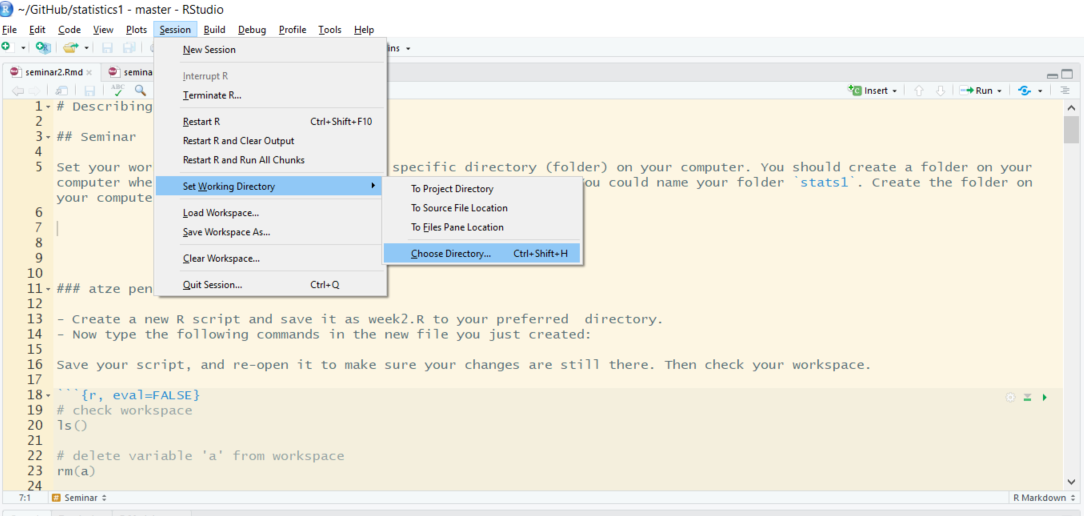
\includegraphics{./img/setwdir.png}
\caption{}
\end{figure}

Create a new R script and save it as week2.R to your \texttt{stats1}
directory. Now type the following commands in the new file you just
created:

\begin{Shaded}
\begin{Highlighting}[]
\CommentTok{# Create a numeric and a character variable}
\NormalTok{a <-}\StringTok{ }\DecValTok{5} \CommentTok{# numeric}
\NormalTok{a <-}\StringTok{ "five"} \CommentTok{# character}
\end{Highlighting}
\end{Shaded}

Save your script, and re-open it to make sure your changes are still
there. Then check your workspace.

\begin{Shaded}
\begin{Highlighting}[]
\CommentTok{# check workspace}
\KeywordTok{ls}\NormalTok{()}

\CommentTok{# delete variable 'a' from workspace}
\KeywordTok{rm}\NormalTok{(a)}

\CommentTok{# delete everything from workspace}
\KeywordTok{rm}\NormalTok{( }\DataTypeTok{list =} \KeywordTok{ls}\NormalTok{() )}

\CommentTok{# to clear console window press Crtl+l on Win or Command+l on Mac}
\end{Highlighting}
\end{Shaded}

\subsection{vectors and subsetting}\label{vectors-and-subsetting}

Last week we have already worked with vectors. We created a sequence for
example. This week, we learn about subsetting (accessing specific
elements of our vector).

We create a vector using the \texttt{c()} function, where c stands for
collect.

\begin{Shaded}
\begin{Highlighting}[]
\CommentTok{# Create a vector}
\NormalTok{my.vector <-}\StringTok{ }\KeywordTok{c}\NormalTok{(}\DecValTok{10}\NormalTok{,}\DecValTok{7}\NormalTok{,}\DecValTok{99}\NormalTok{,}\DecValTok{34}\NormalTok{,}\DecValTok{0}\NormalTok{,}\DecValTok{5}\NormalTok{) }\CommentTok{# a vector}
\NormalTok{my.vector}
\end{Highlighting}
\end{Shaded}

\begin{verbatim}
[1] 10  7 99 34  0  5
\end{verbatim}

Let's see how many elements our vector contains using the
\texttt{length()} function.

\begin{Shaded}
\begin{Highlighting}[]
\KeywordTok{length}\NormalTok{(my.vector) }\CommentTok{# how many elements?}
\end{Highlighting}
\end{Shaded}

\begin{verbatim}
[1] 6
\end{verbatim}

Next, we access the first element in our vector. We use square brackets
to access a specific element. The number in the square brackets is the
vector element that we access

\begin{Shaded}
\begin{Highlighting}[]
\CommentTok{# subsetting}
\NormalTok{my.vector[}\DecValTok{1}\NormalTok{] }\CommentTok{# 1st vector element}
\end{Highlighting}
\end{Shaded}

\begin{verbatim}
[1] 10
\end{verbatim}

To access all elements except the first element, we use the \texttt{-}
operator.

\begin{Shaded}
\begin{Highlighting}[]
\NormalTok{my.vector[}\OperatorTok{-}\DecValTok{1}\NormalTok{] }\CommentTok{# all elements but the 1st}
\end{Highlighting}
\end{Shaded}

\begin{verbatim}
[1]  7 99 34  0  5
\end{verbatim}

We can access elements 2 to 4 by using the colon.

\begin{Shaded}
\begin{Highlighting}[]
\NormalTok{my.vector[}\DecValTok{2}\OperatorTok{:}\DecValTok{4}\NormalTok{] }\CommentTok{# the 2nd to the 4th elements}
\end{Highlighting}
\end{Shaded}

\begin{verbatim}
[1]  7 99 34
\end{verbatim}

We can access two specific non-adjacent elements, by using the collect
function \texttt{c()}.

\begin{Shaded}
\begin{Highlighting}[]
\NormalTok{my.vector[}\KeywordTok{c}\NormalTok{(}\DecValTok{2}\NormalTok{,}\DecValTok{5}\NormalTok{)] }\CommentTok{# 2nd and 5th element}
\end{Highlighting}
\end{Shaded}

\begin{verbatim}
[1] 7 0
\end{verbatim}

No, we combine the \texttt{length()} function with the square brackets
to access the last element in our vector.

\begin{Shaded}
\begin{Highlighting}[]
\NormalTok{my.vector[}\KeywordTok{length}\NormalTok{(my.vector)] }\CommentTok{# the last element}
\end{Highlighting}
\end{Shaded}

\begin{verbatim}
[1] 5
\end{verbatim}

\subsection{data frames}\label{data-frames}

A data frame is an object that holds data in a tabular format similar to
how spreadsheets work. Variables are generally kept in columns and
observations are in rows.

Before we work with ready-made data, we create a small dataset
ourselves. It contains the populations of the sixteen German states. We
start with a vector that contains the names of those states. We call the
variable \emph{state}. Our variable shall contain text instead of
numbers. In R jargon, this is a character variable, sometimes referred
to as a string. Using quotes, we indicate that the variable type is
character. We use the \texttt{c()} function to create the vector.

\begin{Shaded}
\begin{Highlighting}[]
\CommentTok{# create a character vector containing state names}
\NormalTok{state <-}\StringTok{ }\KeywordTok{c}\NormalTok{(}
  \StringTok{"North Rhine-Westphalia"}\NormalTok{,}
  \StringTok{"Bavaria"}\NormalTok{,}
  \StringTok{"Baden-Wurttemberg"}\NormalTok{,}
  \StringTok{"Lower Saxony"}\NormalTok{,}
  \StringTok{"Hesse"}\NormalTok{,}
  \StringTok{"Saxony"}\NormalTok{,}
  \StringTok{"Rhineland-Palatinate"}\NormalTok{,}
  \StringTok{"Berlin"}\NormalTok{,}
  \StringTok{"Schleswig-Holstein"}\NormalTok{,}
  \StringTok{"Brandenburg"}\NormalTok{,}
  \StringTok{"Saxony-Anhalt"}\NormalTok{,}
  \StringTok{"Thuringia"}\NormalTok{,}
  \StringTok{"Hamburg"}\NormalTok{,}
  \StringTok{"Mecklenburg-Vorpommern"}\NormalTok{,}
  \StringTok{"Saarland"}\NormalTok{,}
  \StringTok{"Bremen"}
\NormalTok{  )}
\end{Highlighting}
\end{Shaded}

Now, we create a second variable for the populations. This is a numeric
vector, so we do not use the quotes.

\begin{Shaded}
\begin{Highlighting}[]
\NormalTok{population <-}\StringTok{ }\KeywordTok{c}\NormalTok{(}
  \DecValTok{17865516}\NormalTok{,}
  \DecValTok{12843514}\NormalTok{,}
  \DecValTok{10879618}\NormalTok{,}
  \DecValTok{7926599}\NormalTok{,}
  \DecValTok{6176172}\NormalTok{,}
  \DecValTok{4084851}\NormalTok{,}
  \DecValTok{4052803}\NormalTok{,}
  \DecValTok{3670622}\NormalTok{,}
  \DecValTok{2858714}\NormalTok{,}
  \DecValTok{2484826}\NormalTok{,}
  \DecValTok{2245470}\NormalTok{,}
  \DecValTok{2170714}\NormalTok{,}
  \DecValTok{1787408}\NormalTok{,}
  \DecValTok{1612362}\NormalTok{,}
  \DecValTok{995597}\NormalTok{,}
  \DecValTok{671489}
\NormalTok{)}
\end{Highlighting}
\end{Shaded}

Now with both vectors created, we combine them into a dataframe. We put
our vectors in and give them names. In this case the variable names in
the dataset correspond to our vector names. The name goes in front of
the equal sign and the vector object name, after.

\begin{Shaded}
\begin{Highlighting}[]
\NormalTok{popdata <-}\StringTok{ }\KeywordTok{data.frame}\NormalTok{( }
  \DataTypeTok{state =}\NormalTok{ state,}
  \DataTypeTok{population =}\NormalTok{ population}
\NormalTok{  )}
\end{Highlighting}
\end{Shaded}

You should see the new data frame object in your global environment
window. You can view the dataset in the spreadsheet form that we are all
used to by clicking on the oject name.

We can see the names of variables in our dataset with the names function

\begin{Shaded}
\begin{Highlighting}[]
\KeywordTok{names}\NormalTok{(popdata)}
\end{Highlighting}
\end{Shaded}

\begin{verbatim}
[1] "state"      "population"
\end{verbatim}

Let's check the variable types in our data using the \texttt{str()}
function.

\begin{Shaded}
\begin{Highlighting}[]
\KeywordTok{str}\NormalTok{(popdata)}
\end{Highlighting}
\end{Shaded}

\begin{verbatim}
'data.frame':   16 obs. of  2 variables:
 $ state     : Factor w/ 16 levels "Baden-Wurttemberg",..: 10 2 1 8 7 13 11 3 15 4 ...
 $ population: num  17865516 12843514 10879618 7926599 6176172 ...
\end{verbatim}

The variable \emph{state} is a factor variable. R has turned the
character variable into a categorical variable automatically. The
variable \emph{population} is numeric. These variable types differ. We
can calculate with numeric variables only.

Often we want to access certain observations (rows) or certain columns
(variables) or a combination of the two without looking at the entire
dataset all at once. We can use square brackets to subset data frames.
In square brackets we put a row and a column coordinate separated by a
comma. The row coordinate goes first and the column coordinate second.
So \texttt{popdata{[}10,\ 2{]}} returns the 10th row and second column
of the data frame. If we leave the column coordinate empty this means we
would like all columns. So, \texttt{popdata{[}10,{]}} returns the 10th
row of the dataset. If we leave the row coordinate empty, R returns the
entire column. \texttt{popdata{[},2{]}} returns the second column of the
dataset.

We can look at the first five rows of a dataset to get a better
understanding of it with the colon in brackets like so:
\texttt{popdata{[}1:5,{]}}. We could display the second and fifth
columns of the dataset by using the \texttt{c()} function in brackets
like so: \texttt{popdata{[},\ c(2,5){]}}.

It's your turn. Display all columns of the popdata dataset and show rows
10 to 15. Next display all columns of the dataset and rows 4 and 7.

\begin{Shaded}
\begin{Highlighting}[]
\NormalTok{popdata[}\DecValTok{10}\OperatorTok{:}\DecValTok{15}\NormalTok{, ] }\CommentTok{# elements in 10th to 15th row, all columns}
\end{Highlighting}
\end{Shaded}

\begin{verbatim}
                    state population
10            Brandenburg    2484826
11          Saxony-Anhalt    2245470
12              Thuringia    2170714
13                Hamburg    1787408
14 Mecklenburg-Vorpommern    1612362
15               Saarland     995597
\end{verbatim}

\begin{Shaded}
\begin{Highlighting}[]
\NormalTok{popdata[}\KeywordTok{c}\NormalTok{(}\DecValTok{4}\NormalTok{, }\DecValTok{7}\NormalTok{), ] }\CommentTok{# elements in 4th and 7th row, all column}
\end{Highlighting}
\end{Shaded}

\begin{verbatim}
                 state population
4         Lower Saxony    7926599
7 Rhineland-Palatinate    4052803
\end{verbatim}

In order to access individual columns of a data frame we can also use
the dollar sign \texttt{\$}. For example, let's see how to access the
\texttt{population} column.

\begin{Shaded}
\begin{Highlighting}[]
\NormalTok{popdata}\OperatorTok{$}\NormalTok{population}
\end{Highlighting}
\end{Shaded}

\begin{verbatim}
 [1] 17865516 12843514 10879618  7926599  6176172  4084851  4052803
 [8]  3670622  2858714  2484826  2245470  2170714  1787408  1612362
[15]   995597   671489
\end{verbatim}

Now, access the state column.

\begin{Shaded}
\begin{Highlighting}[]
\NormalTok{popdata}\OperatorTok{$}\NormalTok{state}
\end{Highlighting}
\end{Shaded}

\begin{verbatim}
 [1] North Rhine-Westphalia Bavaria                Baden-Wurttemberg     
 [4] Lower Saxony           Hesse                  Saxony                
 [7] Rhineland-Palatinate   Berlin                 Schleswig-Holstein    
[10] Brandenburg            Saxony-Anhalt          Thuringia             
[13] Hamburg                Mecklenburg-Vorpommern Saarland              
[16] Bremen                
16 Levels: Baden-Wurttemberg Bavaria Berlin Brandenburg Bremen ... Thuringia
\end{verbatim}

\subsection{Loading data}\label{loading-data}

Before you load the dataset into R, you first download it and save it
locally in your \texttt{Stats1} folder. Download the data
\href{http://philippbroniecki.github.io/ML2017.io/data/BSAS_manip.RData}{here}.

We often load existing data sets into R for analysis. Data come in many
different file formats such as \texttt{.csv}, \texttt{.tab},
\texttt{.dta}, etc. Today we will load a dataset which is stored in R's
native file format: \texttt{.RData}. The function to load data from this
file format is called: \texttt{load()}. If you managed to set your
working directory correctly just now
(\texttt{setwd("\textasciitilde{}/Stats1"})), then you should just be
able to run the line of code below.

We load the dataset with the \texttt{load()} function:

\begin{Shaded}
\begin{Highlighting}[]
\CommentTok{# load perception of non-western foreigners data}
\KeywordTok{load}\NormalTok{(}\StringTok{"BSAS_manip.RData"}\NormalTok{)}
\end{Highlighting}
\end{Shaded}

The non-western foreingers data is about the subjective perception of
immigrants from non-western countries. The perception of immigrants from
a context that is not similar to the one's own ,is often used as a proxy
for racism. Whether this is a fair measure or not is debatable but let's
examine the data from a survey carried out in Britain.

Let's check the codebook of our data.

\begin{tabular}{l|l}
\hline
Variable & Description\\
\hline
IMMBRIT & Out of every 100 people in Britain, how many do you think are immigrants from non-western countries?\\
\hline
over.estimate & 1 if estimate is higher than 10.7\%.\\
\hline
RSex & 1 = male, 2 = female\\
\hline
RAge & Age of respondent\\
\hline
Househld & Number of people living in respondent's household\\
\hline
party identification & 1 = Conservatives, 2 = Labour, 3 = SNP, 4 = Greens, 5 = Ukip, 6 = BNP, 7 = other\\
\hline
paper & Do you normally read any daily morning newspaper 3+ times/week?\\
\hline
WWWhourspW & How many hours WWW per week?\\
\hline
religious & Do you regard yourself as belonging to any particular religion?\\
\hline
employMonths & How many mnths w. present employer?\\
\hline
urban & Population density, 4 categories (highest density is 4, lowest is 1)\\
\hline
health.good & How is your health in general for someone of your age? (0: bad, 1: fair, 2: fairly good, 3: good)\\
\hline
HHInc & Income bands for household, high number = high HH income\\
\hline
\end{tabular}

We can look at the variable names in our data with the
\href{http://bit.ly/R_names}{\texttt{names()}} function.

The \href{http://bit.ly/R_dim}{\texttt{dim()}} function can be used to
find out the dimensions of the dataset (dimension 1 = rows, dimension 2
= columns).

\begin{Shaded}
\begin{Highlighting}[]
\KeywordTok{dim}\NormalTok{(data2)}
\end{Highlighting}
\end{Shaded}

\begin{verbatim}
[1] 1049   19
\end{verbatim}

So, the \href{http://bit.ly/R_dim}{\texttt{dim()}} function tells us
that we have data from 1049 respondents with 19 variables for each
respondent.

Let's take a quick peek at the first 10 observations to see what the
dataset looks like. By default the
\href{http://bit.ly/R_head}{\texttt{head()}} function returns the first
6 rows, but let's tell it to return the first 10 rows instead.

\begin{Shaded}
\begin{Highlighting}[]
\KeywordTok{head}\NormalTok{(data2, }\DataTypeTok{n =} \DecValTok{10}\NormalTok{)}
\end{Highlighting}
\end{Shaded}

\begin{verbatim}
   IMMBRIT over.estimate RSex RAge Househld Cons Lab SNP Ukip BNP GP
1        1             0    1   50        2    0   1   0    0   0  0
2       50             1    2   18        3    0   0   0    0   0  0
3       50             1    2   60        1    0   0   0    0   0  0
4       15             1    2   77        2    0   0   0    0   0  0
5       20             1    2   67        1    0   0   0    0   0  0
6       30             1    1   30        4    0   0   0    0   0  0
7       60             1    2   56        2    0   0   1    0   0  0
8        7             0    1   49        1    0   0   0    0   0  0
9       30             1    1   40        4    0   0   1    0   0  0
10       2             0    1   61        3    1   0   0    0   0  0
   party.other paper WWWhourspW religious employMonths urban health.good
1            0     0          1         0           72     4           1
2            1     0          4         0           72     4           2
3            1     0          1         0          456     3           3
4            1     1          2         1           72     1           3
5            1     0          1         1           72     3           3
6            1     1         14         0           72     1           2
7            0     0          5         1          180     1           2
8            1     1          8         0          156     4           2
9            0     0          3         1          264     2           2
10           0     1          0         1           72     1           3
   HHInc
1     13
2      3
3      9
4      8
5      9
6      9
7     13
8     14
9     11
10     8
\end{verbatim}

\subsection{Plots}\label{plots}

We can visualize the data with the help of a boxplot, so let's see how
the perception of the number of immigrants is distributed.

\begin{Shaded}
\begin{Highlighting}[]
\CommentTok{# how good are we at guessing immigration}
\KeywordTok{boxplot}\NormalTok{(}
\NormalTok{  data2}\OperatorTok{$}\NormalTok{IMMBRIT, }
  \DataTypeTok{main =} \StringTok{"Perception of Immigration from Non-Western Countries"}\NormalTok{,}
  \DataTypeTok{ylab =} \StringTok{"Subjective number of immigrants per 100 British"}\NormalTok{, }
  \DataTypeTok{frame.plot =} \OtherTok{FALSE}\NormalTok{, }\DataTypeTok{col =} \StringTok{"darkgray"}
\NormalTok{  )}
\end{Highlighting}
\end{Shaded}

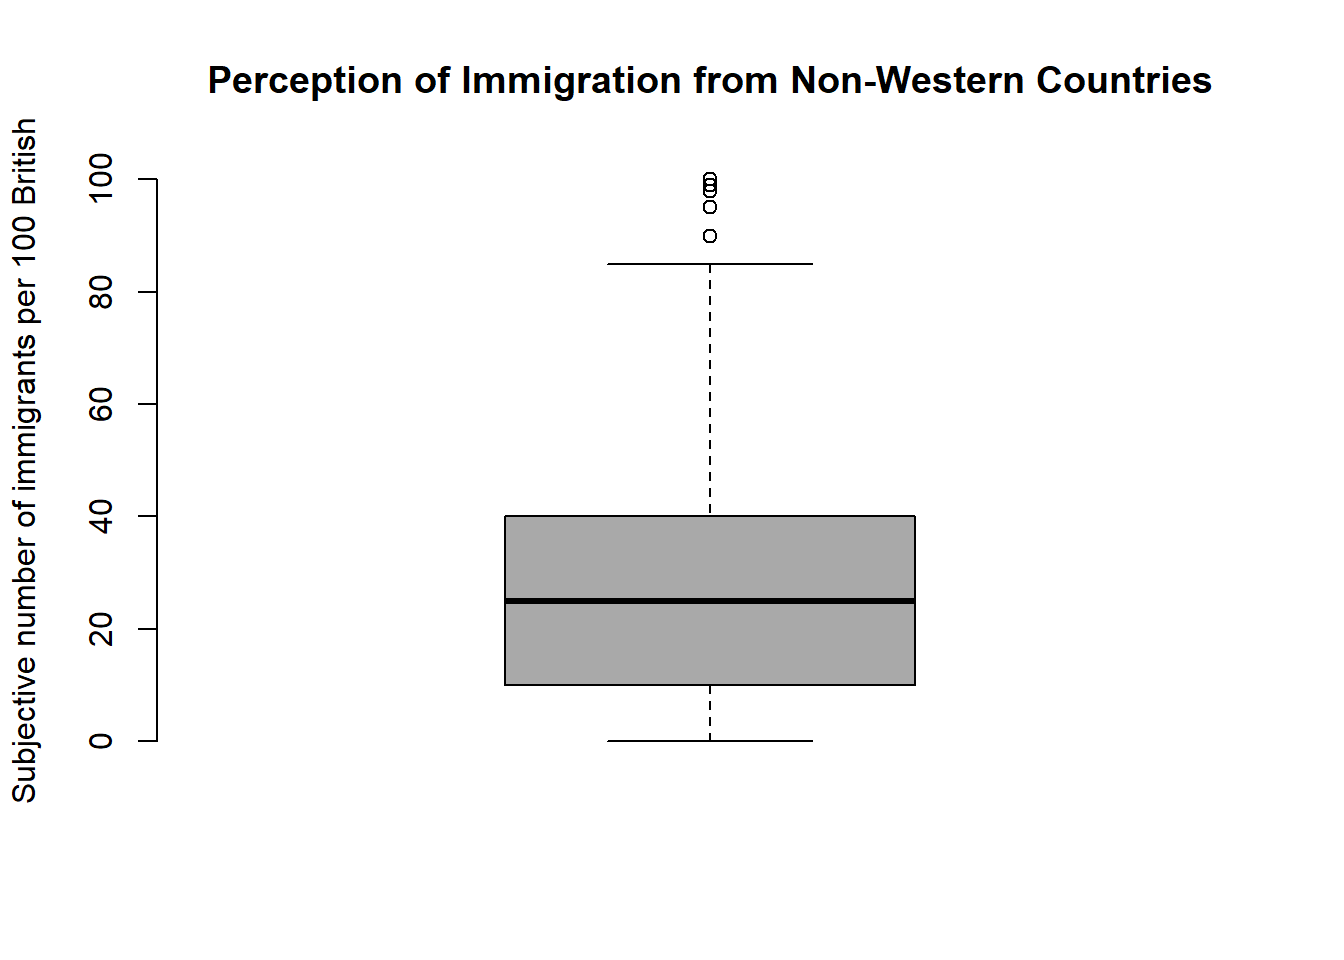
\includegraphics{statistics1_files/figure-latex/unnamed-chunk-69-1.pdf}

Notice how the lower whisker is much shorter than the upper one. The
distribution is right skewed. The right tail (higher values) is a lot
longer. We can see this beter using a density plot. We combine R's
\texttt{denisty()} function with the \texttt{plot()} function.

\begin{Shaded}
\begin{Highlighting}[]
\KeywordTok{plot}\NormalTok{(}
  \KeywordTok{density}\NormalTok{(data2}\OperatorTok{$}\NormalTok{IMMBRIT),}
  \DataTypeTok{bty =} \StringTok{"n"}\NormalTok{,}
  \DataTypeTok{main =} \StringTok{"Perception of Immigration from Non-Western Countries"}\NormalTok{,}
  \DataTypeTok{xlab =} \StringTok{"Subjective number of immigrants per 100 British"}
\NormalTok{  )}
\end{Highlighting}
\end{Shaded}

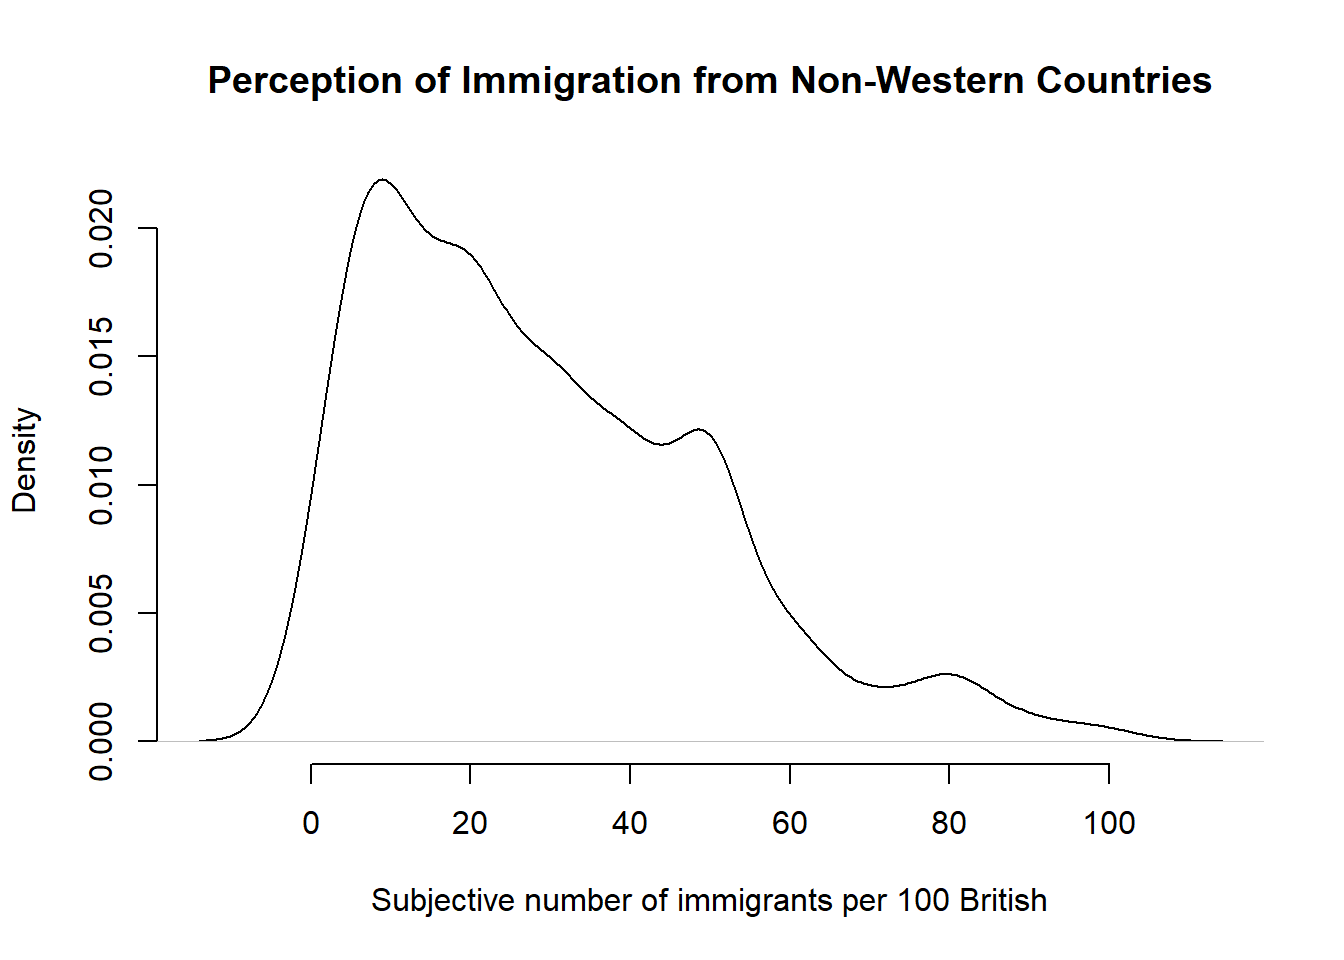
\includegraphics{statistics1_files/figure-latex/unnamed-chunk-70-1.pdf}

We can also plot histograms using the \texttt{hist()} function.

\begin{Shaded}
\begin{Highlighting}[]
\CommentTok{# histogram}
\KeywordTok{hist}\NormalTok{( data2}\OperatorTok{$}\NormalTok{employMonths, }\DataTypeTok{main =} \StringTok{"histogram"}\NormalTok{)}
\end{Highlighting}
\end{Shaded}

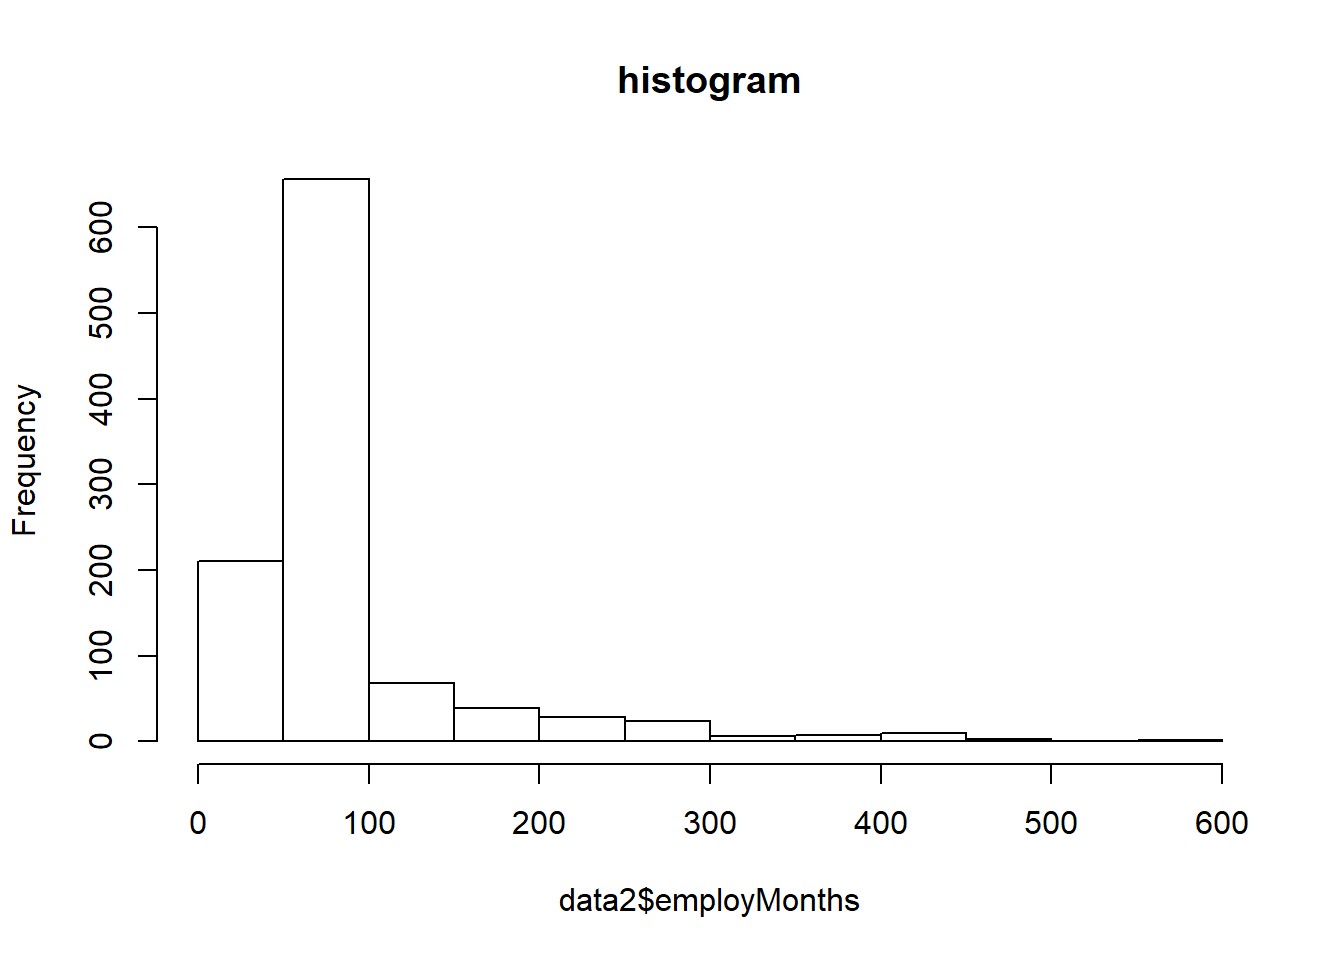
\includegraphics{statistics1_files/figure-latex/unnamed-chunk-71-1.pdf}

It is plausible that perception of immigration from Non-Western
countries is related to party affiliation. In our dataset, we have a
some party affiliation dummies (binary variables). We can use square
brackets to subset our data such that we produce a boxplot only for
members of the Conservative Party. We have a look at the variable
\emph{Cons} using the \texttt{table()} function first.

\begin{Shaded}
\begin{Highlighting}[]
\KeywordTok{table}\NormalTok{(data2}\OperatorTok{$}\NormalTok{Cons)}
\end{Highlighting}
\end{Shaded}

\begin{verbatim}

  0   1 
765 284 
\end{verbatim}

In our data, 284 respondents associate with the Conservative party and
765 do not. We create a boxplot of \emph{IMMBRIT} but only for members
of the Conservative Party. We do so by using the square brackets to
subset our data.

\begin{Shaded}
\begin{Highlighting}[]
\CommentTok{# boxplot of immbrit for those observations where Cons is 1}
\KeywordTok{boxplot}\NormalTok{(}
\NormalTok{  data2}\OperatorTok{$}\NormalTok{IMMBRIT[data2}\OperatorTok{$}\NormalTok{Cons}\OperatorTok{==}\DecValTok{1}\NormalTok{],}
  \DataTypeTok{frame.plot =} \OtherTok{FALSE}\NormalTok{,}
  \DataTypeTok{xlab =} \StringTok{"Conservatives"}\NormalTok{,}
  \DataTypeTok{col =} \StringTok{"blue"}
\NormalTok{  )}
\end{Highlighting}
\end{Shaded}

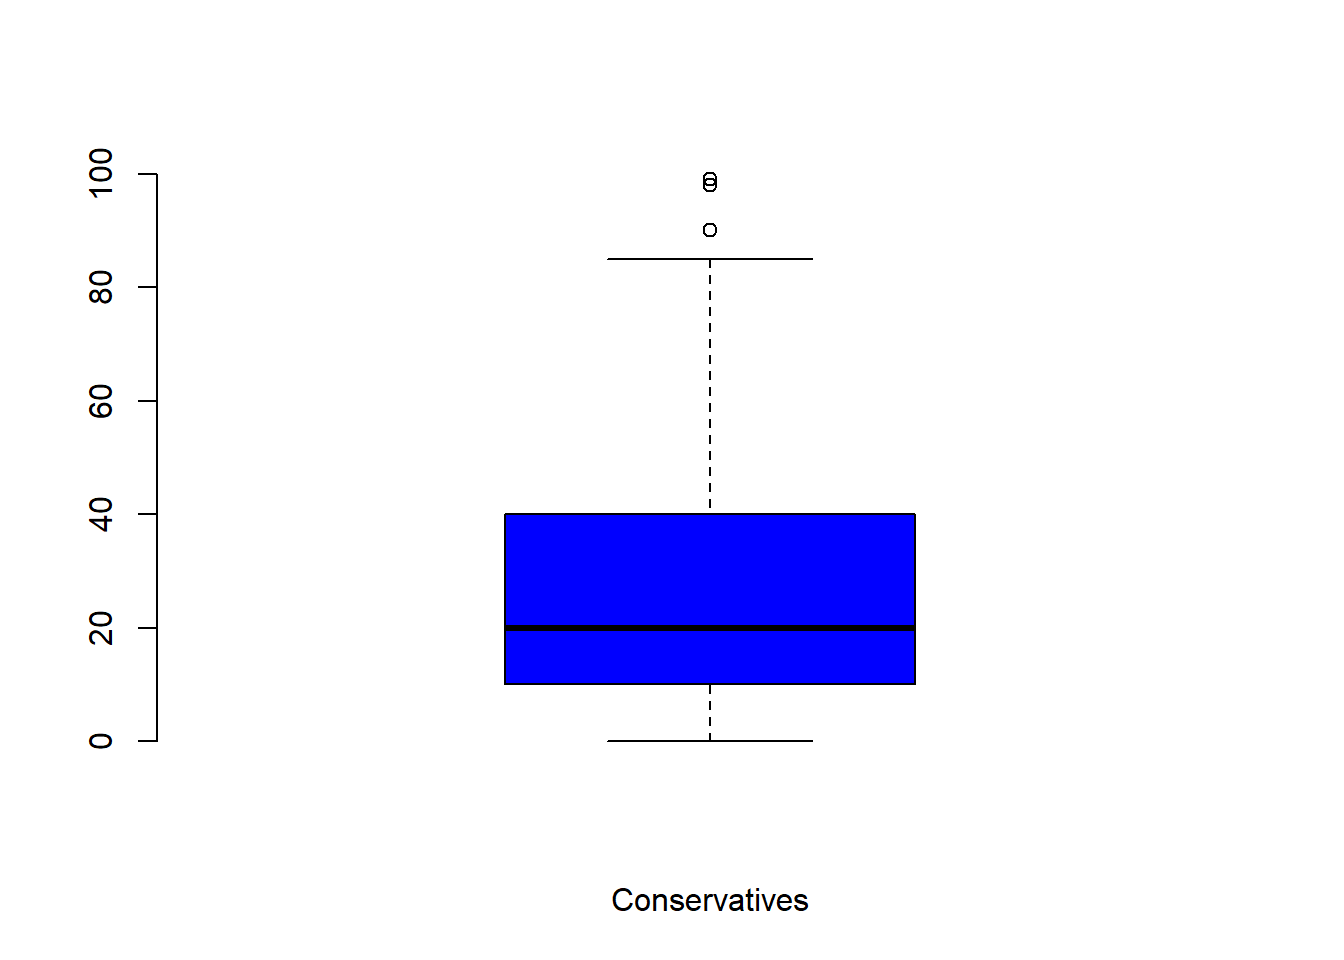
\includegraphics{statistics1_files/figure-latex/unnamed-chunk-73-1.pdf}

We would now like to compare the distribution of the perception fo
Conservatives to the distribution among Labour respondents. We can
subset the data just like we did for the Conservative Party. In addtion,
we want to plot the two plots next to each other, i.e., they should be
in the same plot. We can achieve this with the \texttt{par()} function
and the \texttt{mfrow} argument. This will spilt the plot window into
rows and columns. We want 2 columns to plot 2 boxplots next to each
other.

\begin{Shaded}
\begin{Highlighting}[]
\CommentTok{# split plot window into 1 row and 2 columns}
\KeywordTok{par}\NormalTok{(}\DataTypeTok{mfrow =} \KeywordTok{c}\NormalTok{(}\DecValTok{1}\NormalTok{,}\DecValTok{2}\NormalTok{))}

\CommentTok{# plot 1}
\KeywordTok{boxplot}\NormalTok{(}
\NormalTok{  data2}\OperatorTok{$}\NormalTok{IMMBRIT[data2}\OperatorTok{$}\NormalTok{Cons}\OperatorTok{==}\DecValTok{1}\NormalTok{],}
  \DataTypeTok{frame.plot =} \OtherTok{FALSE}\NormalTok{,}
  \DataTypeTok{xlab =} \StringTok{"Conservatives"}\NormalTok{,}
  \DataTypeTok{col =} \StringTok{"blue"}
\NormalTok{  )}

\CommentTok{# plot 2}
\KeywordTok{boxplot}\NormalTok{(}
\NormalTok{  data2}\OperatorTok{$}\NormalTok{IMMBRIT[data2}\OperatorTok{$}\NormalTok{Lab}\OperatorTok{==}\DecValTok{1}\NormalTok{],}
  \DataTypeTok{frame.plot =} \OtherTok{FALSE}\NormalTok{,}
  \DataTypeTok{xlab =} \StringTok{"Labour"}\NormalTok{,}
  \DataTypeTok{col =} \StringTok{"red"}
\NormalTok{  )}
\end{Highlighting}
\end{Shaded}

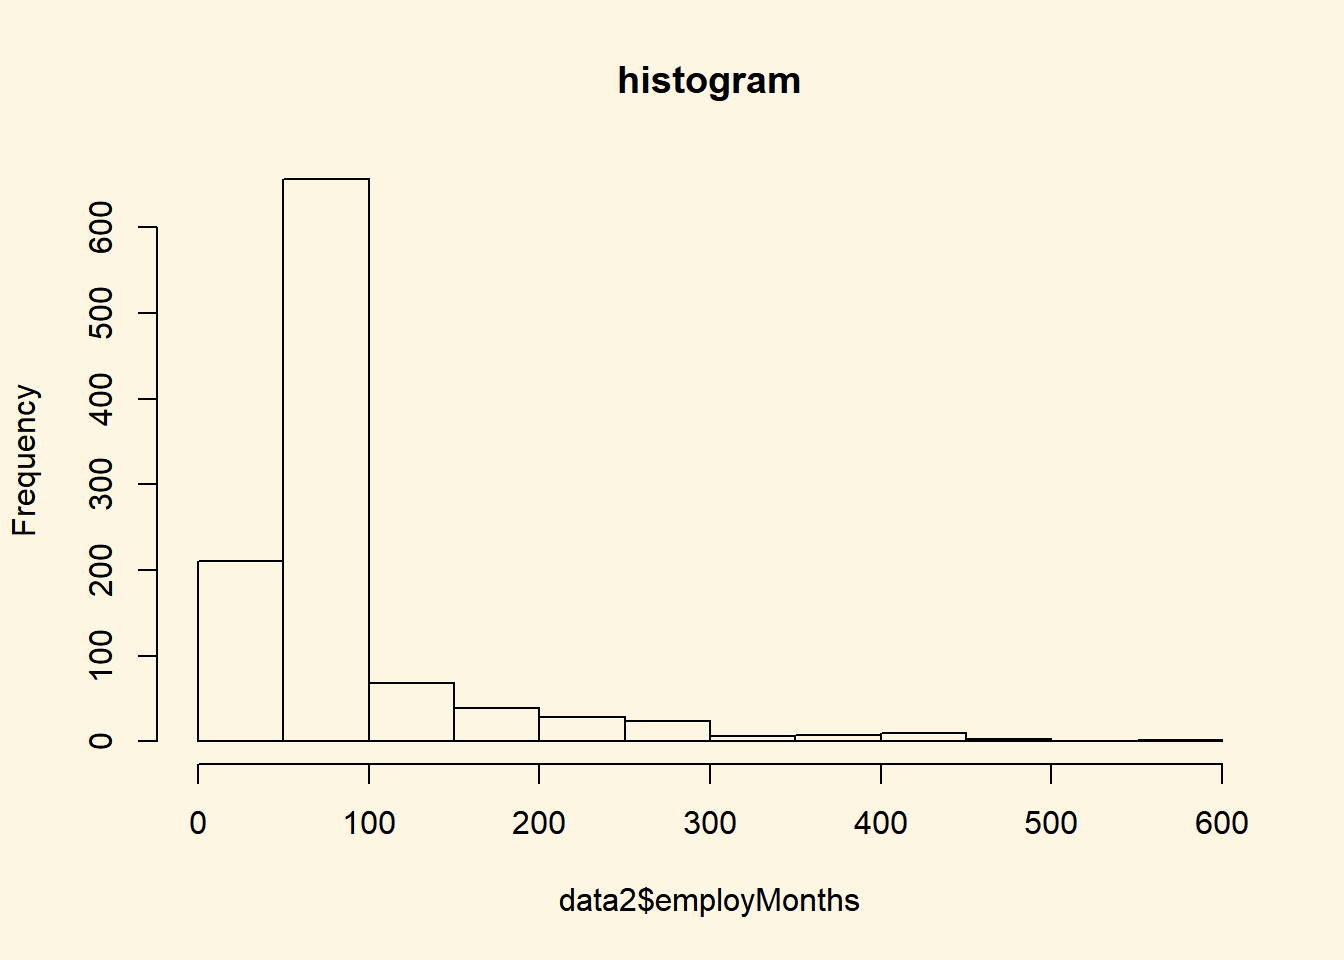
\includegraphics{statistics1_files/figure-latex/unnamed-chunk-74-1.pdf}

It is very hard to spot differences. The distributions are similar. The
median for Labour respondents is larger which mean that the central
Labour respondent over-estimates immigration more than the central
Conservative respondent.

You can play around with the non-western foreigners data on your own
time. We now turn to a dataset that is integrated in R already. It is
called \texttt{longley}. Use the \texttt{help()} function to see what
this dataset is about.

\begin{Shaded}
\begin{Highlighting}[]
\KeywordTok{help}\NormalTok{(longley)}
\end{Highlighting}
\end{Shaded}

Let's create a scatterplot with the \texttt{Year} variable on the x-axis
and \texttt{Employed} on the y-axis.

\begin{Shaded}
\begin{Highlighting}[]
\KeywordTok{plot}\NormalTok{(}\DataTypeTok{x =}\NormalTok{ longley}\OperatorTok{$}\NormalTok{Year, }\CommentTok{# x-axis variable}
     \DataTypeTok{y =}\NormalTok{ longley}\OperatorTok{$}\NormalTok{Employed, }\CommentTok{# y-axis variable}
     \DataTypeTok{bty =} \StringTok{"n"} \CommentTok{# no box around the plot}
\NormalTok{     )}
\end{Highlighting}
\end{Shaded}

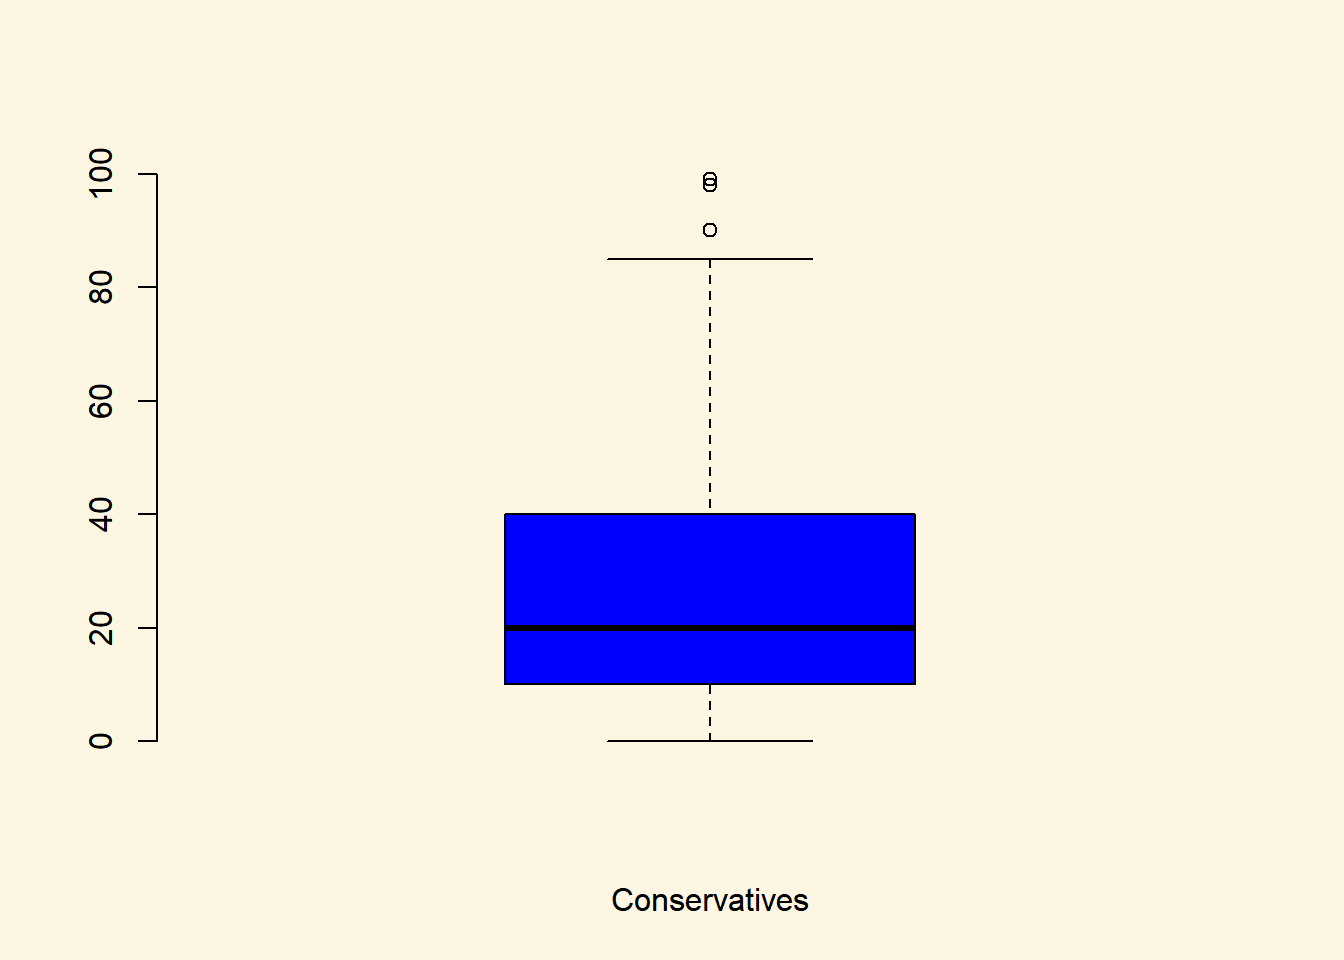
\includegraphics{statistics1_files/figure-latex/unnamed-chunk-76-1.pdf}

To create a line plot instead, we use the same function with one
additional argument \texttt{type\ =\ "l"}.

\begin{Shaded}
\begin{Highlighting}[]
\KeywordTok{plot}\NormalTok{(longley}\OperatorTok{$}\NormalTok{Year, longley}\OperatorTok{$}\NormalTok{Employed, }\DataTypeTok{type =} \StringTok{"l"}\NormalTok{)}
\end{Highlighting}
\end{Shaded}

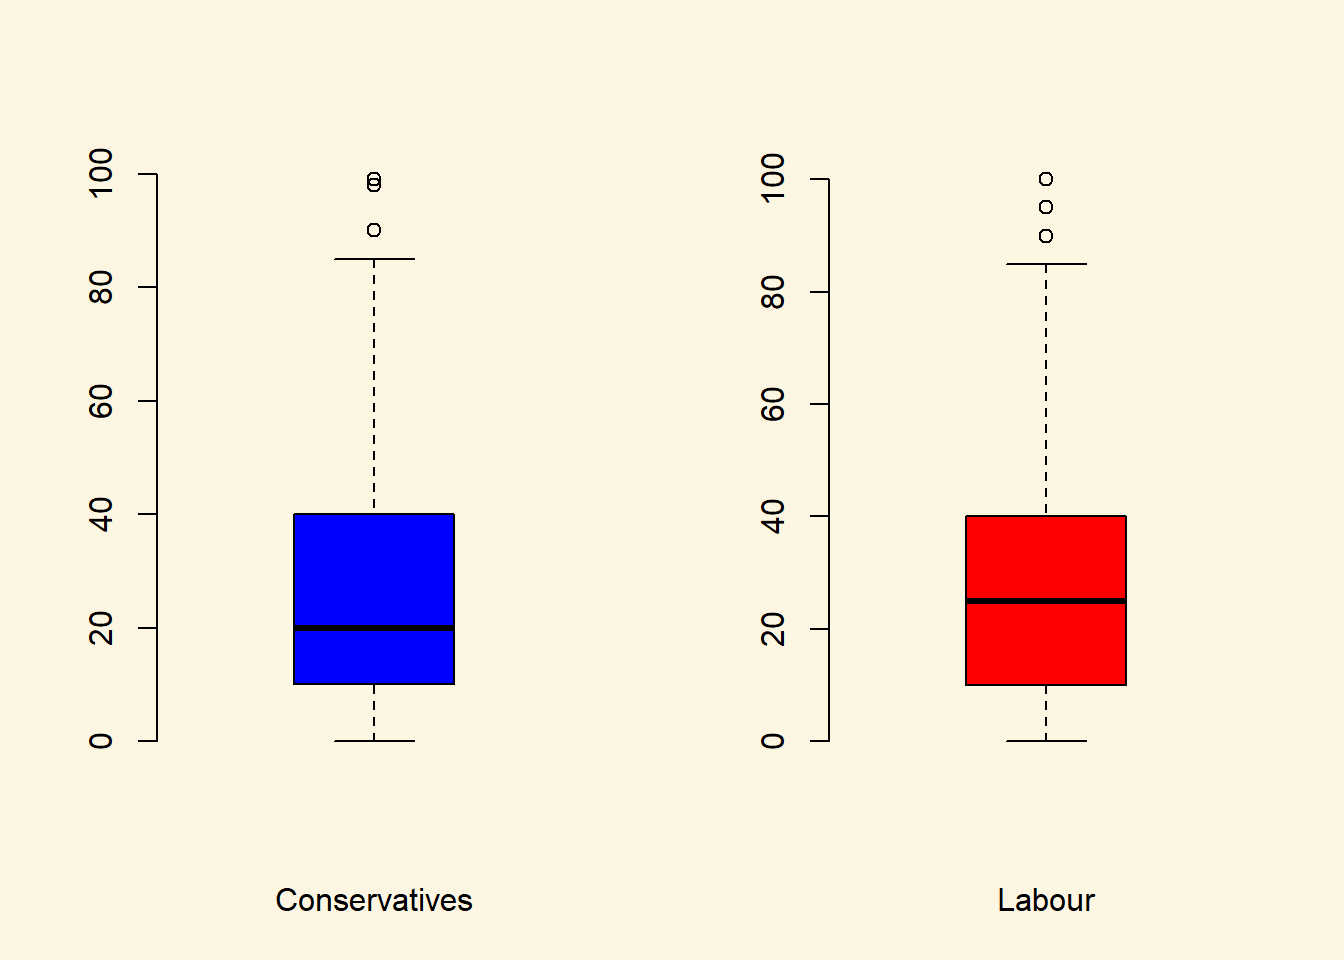
\includegraphics{statistics1_files/figure-latex/unnamed-chunk-77-1.pdf}

Create a plot that includes both points and lines.

\begin{Shaded}
\begin{Highlighting}[]
\KeywordTok{plot}\NormalTok{(longley}\OperatorTok{$}\NormalTok{Year, longley}\OperatorTok{$}\NormalTok{Employed, }\DataTypeTok{type =} \StringTok{"b"}\NormalTok{)}
\end{Highlighting}
\end{Shaded}

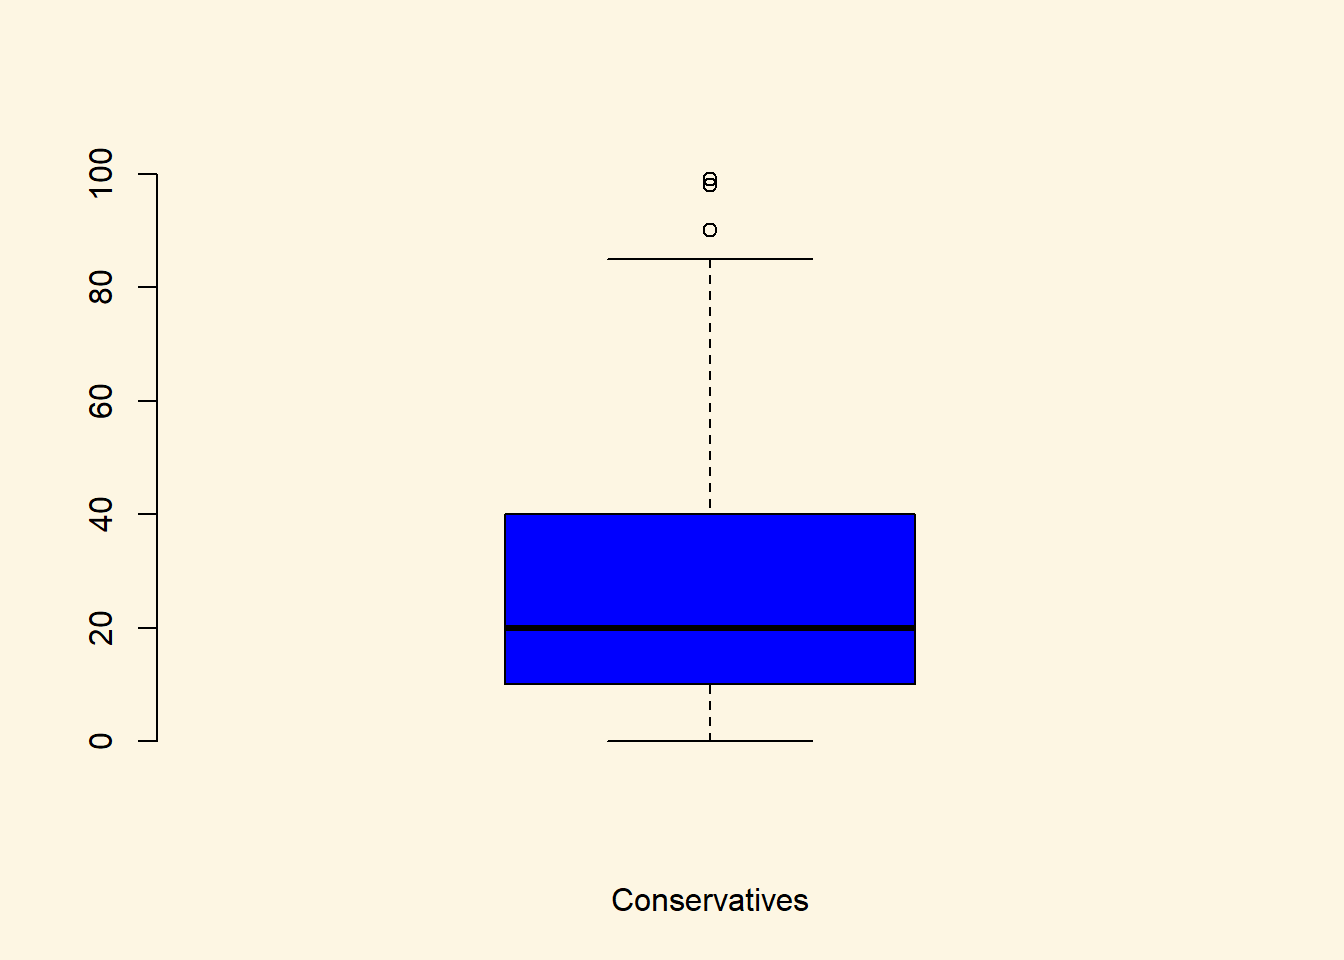
\includegraphics{statistics1_files/figure-latex/unnamed-chunk-78-1.pdf}

\subsection{Average Treatment Effect}\label{average-treatment-effect}

In the lecture, we estimated the average treatment effect on a small
example. We will do this again here. Recall, that the average treatment
effect is the difference between two means.

Let's suppose, associating with right-wing parties causes people to
over-estimate the number of non-western foreigners. Our treatment
variable is whether a respondent assoicates with the UK Independence
Party. It is 1 if that is the case and 0 otherwise. Let's inspect the
variable \emph{Ukip}.

\begin{Shaded}
\begin{Highlighting}[]
\KeywordTok{table}\NormalTok{(data2}\OperatorTok{$}\NormalTok{Ukip)}
\end{Highlighting}
\end{Shaded}

\begin{verbatim}

   0    1 
1018   31 
\end{verbatim}

31 respondents identify with Ukip.

The average treatment effect, as we learned, would be the difference
between the mean outcomes for those who received the treament minus the
mean for those who did not reicive the treatment.

We have all the tools to solve the problem. Let's take the mean of the
treated group first.

\begin{Shaded}
\begin{Highlighting}[]
\NormalTok{mean.y.treated <-}\StringTok{ }\KeywordTok{mean}\NormalTok{(data2}\OperatorTok{$}\NormalTok{IMMBRIT[data2}\OperatorTok{$}\NormalTok{Ukip }\OperatorTok{==}\StringTok{ }\DecValTok{1}\NormalTok{])}
\NormalTok{mean.y.treated}
\end{Highlighting}
\end{Shaded}

\begin{verbatim}
[1] 24.29032
\end{verbatim}

The double equal sign \texttt{==} is a logical operator and means ``is
equal to''. R returns true or false depending on whether the respondent
does identify with Ukip or not. The mean of \emph{IMMBRIT} is then
computed only for respondents who accociate with Ukip.

Let's take the mean of the second group, the untreated group.

\begin{Shaded}
\begin{Highlighting}[]
\NormalTok{mean.y.untreated <-}\StringTok{ }\KeywordTok{mean}\NormalTok{(data2}\OperatorTok{$}\NormalTok{IMMBRIT[data2}\OperatorTok{$}\NormalTok{Ukip }\OperatorTok{==}\StringTok{ }\DecValTok{0}\NormalTok{])}
\NormalTok{mean.y.untreated}
\end{Highlighting}
\end{Shaded}

\begin{verbatim}
[1] 29.17485
\end{verbatim}

The treatment effect is the difference in means:

\begin{Shaded}
\begin{Highlighting}[]
\NormalTok{mean.y.treated }\OperatorTok{-}\StringTok{ }\NormalTok{mean.y.untreated}
\end{Highlighting}
\end{Shaded}

\begin{verbatim}
[1] -4.88453
\end{verbatim}

The result is surprising. Ukip members over-estimate the number of
non-western foreigners less members of all other paries. Our claim is
not quite supported by the data. We should be very careful with these
results, however. We used experimental language but our data is
observational. A multitude of confounders could bias our estimate of the
causal effect.

\subsection{Exercises}\label{exercises-1}

\begin{enumerate}
\def\labelenumi{\arabic{enumi}.}
\tightlist
\item
  Create a script and call it assignment02. Save your script.
\item
  Use the \texttt{names()} function to display the variable names of the
  \texttt{longley} dataset.
\item
  Use square brackets to access the 4th column of the dataset.
\item
  Use the dollar sign to access the 4th column of the dataset.
\item
  Access the two cells from row 4 and column 1 and row 6 and column 3.
\item
  Using the \texttt{longley} data produce a line plot with GNP on the
  y-axis and population on the x-axis.
\item
  Use the help function to find out how to label the y-axis ``wealth''
  and the x-axis ``population''.
\item
  Create a boxplot showing the distribution of \emph{IMMBRIT} by each
  party in the data and plot these in one plot next to each other.
\item
  Is there a difference between women and men in terms of their
  subjective estimation of foreingers?
\item
  What is the difference between women and men?
\item
  Could you form a hypothesis out of the relationship that you see if
  any exists?
\item
  Save your script, which should now include the answers to all the
  exercises.
\item
  Source your script, i.e.~run the entire script without error message.
  Clean your script if you get error messages.
\end{enumerate}

\section{Solutions}\label{solutions-1}

\subsection{Exercise 2}\label{exercise-2}

Use the \texttt{names()} function to display the variable names of the
\texttt{longley} dataset.

\begin{Shaded}
\begin{Highlighting}[]
\KeywordTok{names}\NormalTok{(longley)}
\end{Highlighting}
\end{Shaded}

\begin{verbatim}
[1] "GNP.deflator" "GNP"          "Unemployed"   "Armed.Forces"
[5] "Population"   "Year"         "Employed"    
\end{verbatim}

\subsection{Exercise 3}\label{exercise-3-1}

Use square brackets to access the 4th column of the dataset.

\begin{Shaded}
\begin{Highlighting}[]
\NormalTok{longley[, }\DecValTok{4}\NormalTok{]}
\end{Highlighting}
\end{Shaded}

\begin{verbatim}
 [1] 159.0 145.6 161.6 165.0 309.9 359.4 354.7 335.0 304.8 285.7 279.8
[12] 263.7 255.2 251.4 257.2 282.7
\end{verbatim}

\subsection{Exercise 4}\label{exercise-4-1}

Use the dollar sign to access the 4th column of the dataset.

\begin{Shaded}
\begin{Highlighting}[]
\NormalTok{longley}\OperatorTok{$}\NormalTok{Armed.Forces}
\end{Highlighting}
\end{Shaded}

\begin{verbatim}
 [1] 159.0 145.6 161.6 165.0 309.9 359.4 354.7 335.0 304.8 285.7 279.8
[12] 263.7 255.2 251.4 257.2 282.7
\end{verbatim}

Note: There is yet another way to access the 4th column of the dataset.
We can put the variable name into the square brackets using quotes like
so:

\begin{Shaded}
\begin{Highlighting}[]
\NormalTok{longley[, }\StringTok{"Armed.Forces"}\NormalTok{]}
\end{Highlighting}
\end{Shaded}

\begin{verbatim}
 [1] 159.0 145.6 161.6 165.0 309.9 359.4 354.7 335.0 304.8 285.7 279.8
[12] 263.7 255.2 251.4 257.2 282.7
\end{verbatim}

\subsection{Exercise 5}\label{exercise-5-1}

Access the two cells from row 4 and column 1 and row 6 and column 3.

\begin{Shaded}
\begin{Highlighting}[]
\CommentTok{# row 4, column 1}
\NormalTok{longley[}\DecValTok{4}\NormalTok{, }\DecValTok{1}\NormalTok{]}
\end{Highlighting}
\end{Shaded}

\begin{verbatim}
[1] 89.5
\end{verbatim}

\begin{Shaded}
\begin{Highlighting}[]
\CommentTok{# row 6, column 3}
\NormalTok{longley[}\DecValTok{6}\NormalTok{, }\DecValTok{3}\NormalTok{]}
\end{Highlighting}
\end{Shaded}

\begin{verbatim}
[1] 193.2
\end{verbatim}

\subsection{Exercise 6}\label{exercise-6-1}

Using the \texttt{longley} data produce a line plot with GNP on the
y-axis and population on the x-axis.

\begin{Shaded}
\begin{Highlighting}[]
\KeywordTok{plot}\NormalTok{(}
  \DataTypeTok{y =}\NormalTok{ longley}\OperatorTok{$}\NormalTok{GNP, }\CommentTok{# y-axis variable}
  \DataTypeTok{x =}\NormalTok{ longley}\OperatorTok{$}\NormalTok{Population, }\CommentTok{# x-axis variable}
  \DataTypeTok{type =} \StringTok{"l"}\NormalTok{, }\CommentTok{# produce a line plot}
  \DataTypeTok{bty =} \StringTok{"n"}\NormalTok{, }\CommentTok{# no box around our plot}
  \DataTypeTok{main =} \StringTok{"Relationship of Population Size and Size of the Economy"}
\NormalTok{)}
\end{Highlighting}
\end{Shaded}

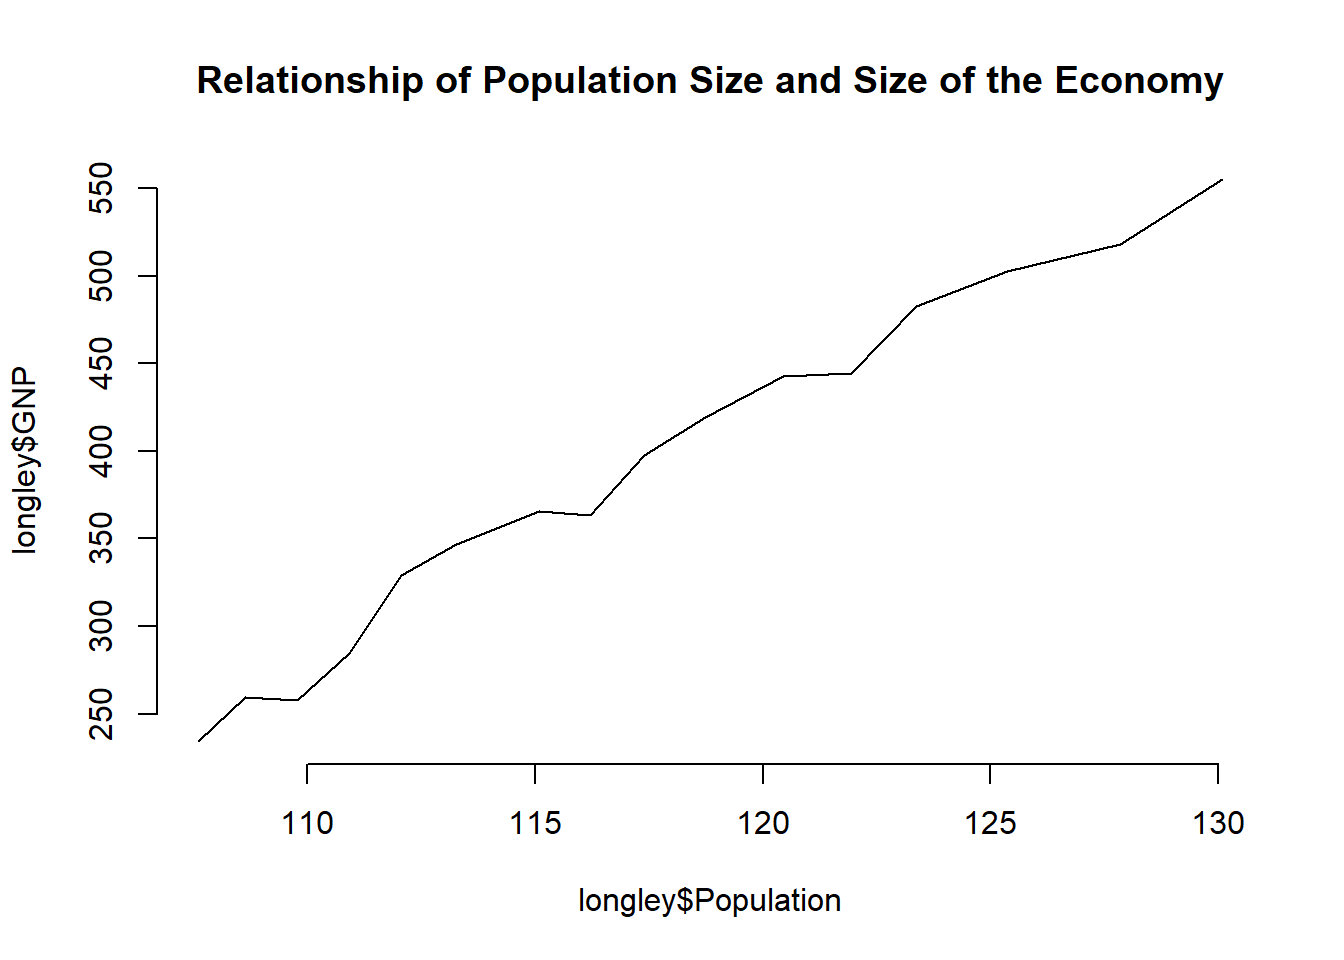
\includegraphics{statistics1_files/figure-latex/unnamed-chunk-89-1.pdf}

\subsection{Exercise 7}\label{exercise-7-1}

Use the help function to find out how to label the y-axis ``wealth'' and
the x-axis ``population''.

\begin{Shaded}
\begin{Highlighting}[]
\NormalTok{?plot}
\end{Highlighting}
\end{Shaded}

The \texttt{?} is short for the \texttt{help()} function. We see that
the \texttt{xlab} argument lets us label the x-axis and the
\texttt{ylab} argument lets us label the y-axis. We do so below.

\begin{Shaded}
\begin{Highlighting}[]
\KeywordTok{plot}\NormalTok{(}
  \DataTypeTok{y =}\NormalTok{ longley}\OperatorTok{$}\NormalTok{GNP, }\CommentTok{# y-axis variable}
  \DataTypeTok{x =}\NormalTok{ longley}\OperatorTok{$}\NormalTok{Population, }\CommentTok{# x-axis variable}
  \DataTypeTok{type =} \StringTok{"l"}\NormalTok{, }\CommentTok{# produce a line plot}
  \DataTypeTok{bty =} \StringTok{"n"}\NormalTok{, }\CommentTok{# no box around our plot}
  \DataTypeTok{main =} \StringTok{"Relationship of Population Size and Size of the Economy"}\NormalTok{,}
  \DataTypeTok{xlab =} \StringTok{"Population older than 14 years of age"}\NormalTok{,}
  \DataTypeTok{ylab =} \StringTok{"Gross national product"}
\NormalTok{)}
\end{Highlighting}
\end{Shaded}

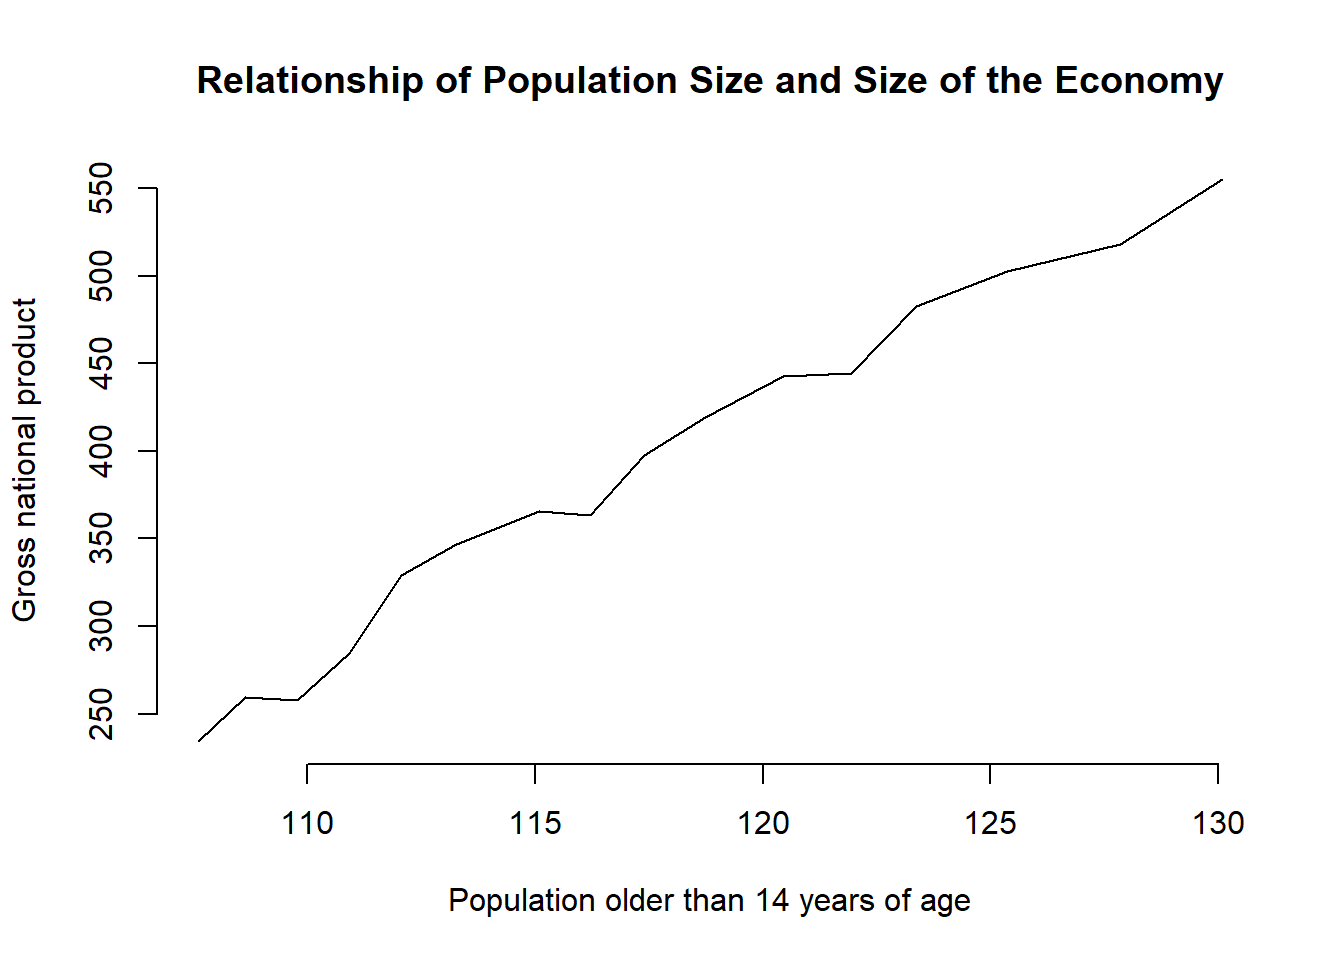
\includegraphics{statistics1_files/figure-latex/unnamed-chunk-91-1.pdf}

\subsection{Exercise 8}\label{exercise-8-1}

Create a boxplot showing the distribution of \emph{IMMBRIT} by each
party in the data and plot these in one plot next to each other.

To do that, we load the non-western foreigners dataset first.

Note: You have to set your working directory that R operates in to the
location of the dataset.

\begin{Shaded}
\begin{Highlighting}[]
\CommentTok{# load perception of non-western foreigners data}
\KeywordTok{load}\NormalTok{(}\StringTok{"BSAS_manip.RData"}\NormalTok{)}
\end{Highlighting}
\end{Shaded}

We have five parties in our dataset. We plot 5 boxplots next to each
other. Hence, we separate the plot window into 1 row and 5 columns.

\begin{Shaded}
\begin{Highlighting}[]
\CommentTok{# plot window to 1 row and 5 columns}
\KeywordTok{par}\NormalTok{(}\DataTypeTok{mfrow =} \KeywordTok{c}\NormalTok{(}\DecValTok{1}\NormalTok{, }\DecValTok{5}\NormalTok{))}
\KeywordTok{boxplot}\NormalTok{(data2}\OperatorTok{$}\NormalTok{IMMBRIT[ data2}\OperatorTok{$}\NormalTok{Cons }\OperatorTok{==}\StringTok{ }\DecValTok{1}\NormalTok{ ], }\DataTypeTok{frame.plot =} \OtherTok{FALSE}\NormalTok{, }\DataTypeTok{col =} \StringTok{"blue"}\NormalTok{, }\DataTypeTok{xlab =} \StringTok{"Tories"}\NormalTok{)}
\KeywordTok{boxplot}\NormalTok{(data2}\OperatorTok{$}\NormalTok{IMMBRIT[ data2}\OperatorTok{$}\NormalTok{Lab }\OperatorTok{==}\StringTok{ }\DecValTok{1}\NormalTok{ ], }\DataTypeTok{frame.plot =} \OtherTok{FALSE}\NormalTok{, }\DataTypeTok{col =} \StringTok{"red"}\NormalTok{, }\DataTypeTok{xlab =} \StringTok{"Labour"}\NormalTok{)}
\KeywordTok{boxplot}\NormalTok{(data2}\OperatorTok{$}\NormalTok{IMMBRIT[ data2}\OperatorTok{$}\NormalTok{SNP }\OperatorTok{==}\StringTok{ }\DecValTok{1}\NormalTok{ ], }\DataTypeTok{frame.plot =} \OtherTok{FALSE}\NormalTok{, }\DataTypeTok{col =} \StringTok{"yellow"}\NormalTok{, }\DataTypeTok{xlab =} \StringTok{"SNP"}\NormalTok{)}
\KeywordTok{boxplot}\NormalTok{(data2}\OperatorTok{$}\NormalTok{IMMBRIT[ data2}\OperatorTok{$}\NormalTok{Ukip }\OperatorTok{==}\StringTok{ }\DecValTok{1}\NormalTok{ ], }\DataTypeTok{frame.plot =} \OtherTok{FALSE}\NormalTok{, }\DataTypeTok{col =} \StringTok{"purple"}\NormalTok{, }\DataTypeTok{xlab =} \StringTok{"Ukip"}\NormalTok{)}
\KeywordTok{boxplot}\NormalTok{(data2}\OperatorTok{$}\NormalTok{IMMBRIT[ data2}\OperatorTok{$}\NormalTok{BNP }\OperatorTok{==}\StringTok{ }\DecValTok{1}\NormalTok{ ], }\DataTypeTok{frame.plot =} \OtherTok{FALSE}\NormalTok{, }\DataTypeTok{col =} \StringTok{"darkblue"}\NormalTok{, }\DataTypeTok{xlab =} \StringTok{"BNP"}\NormalTok{)}
\end{Highlighting}
\end{Shaded}

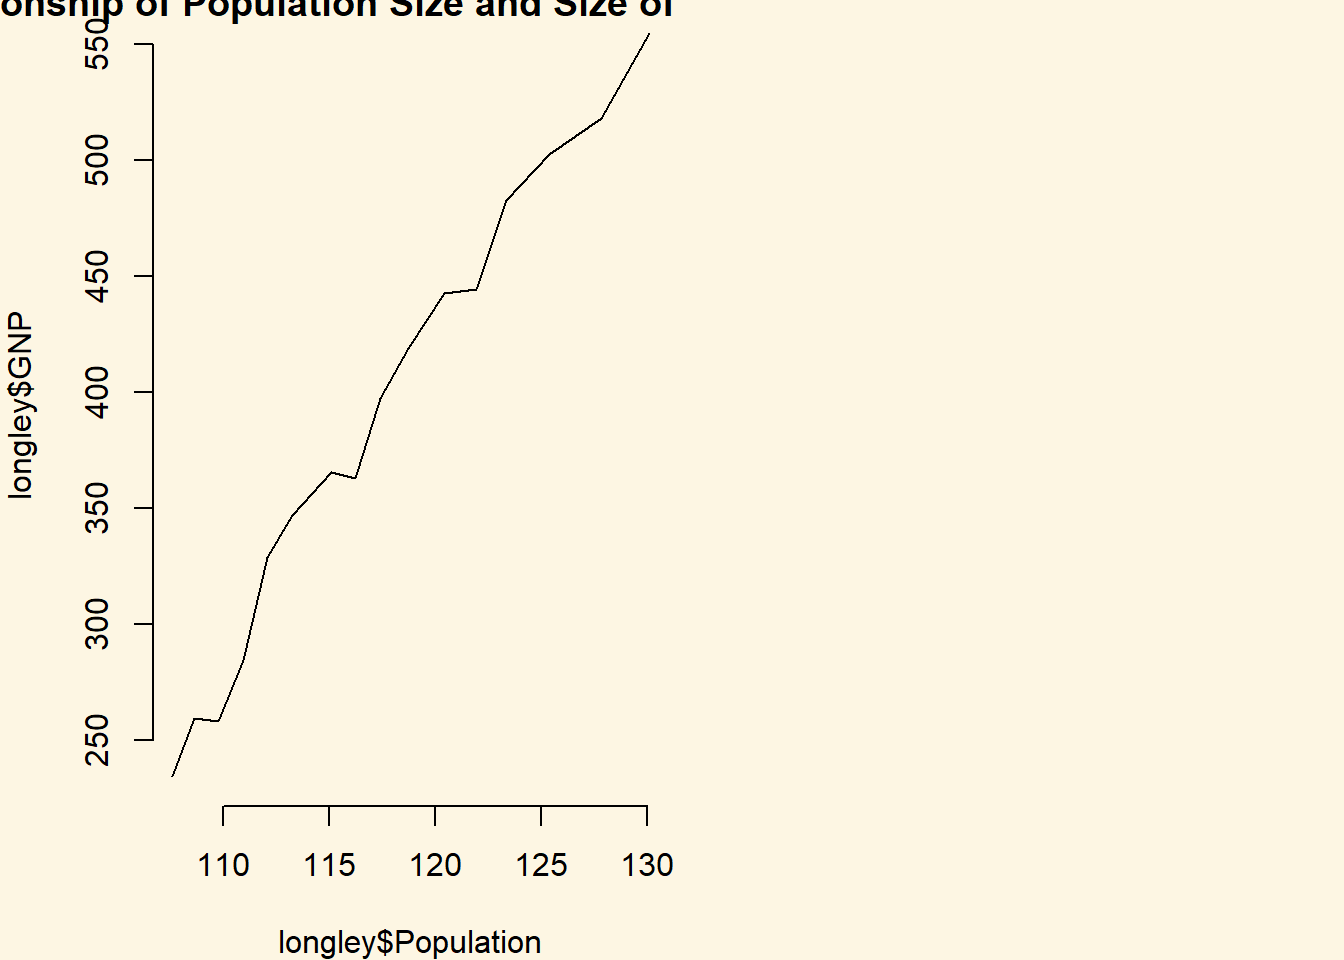
\includegraphics{statistics1_files/figure-latex/unnamed-chunk-93-1.pdf}

\subsection{Exercises 9 and 10}\label{exercises-9-and-10}

We combine the answer to questions 9 and 10.

Question from 9: Is there a difference between women and men in terms of
their subjective estimation of foreingers?

Question from 10: What is the difference between women and men?

Women's subjective estimate is the mean of \emph{IMMBRIT} across women
and equally, men's subjective estimate is the mean of \emph{IMMBRIT}
over all men. Let's get these numbers with the mean function and the
square brackets.

\begin{Shaded}
\begin{Highlighting}[]
\NormalTok{womens.mean <-}\StringTok{ }\KeywordTok{mean}\NormalTok{(data2}\OperatorTok{$}\NormalTok{IMMBRIT[ data2}\OperatorTok{$}\NormalTok{RSex }\OperatorTok{==}\StringTok{ }\DecValTok{2}\NormalTok{ ])}
\NormalTok{womens.mean}
\end{Highlighting}
\end{Shaded}

\begin{verbatim}
[1] 32.79159
\end{verbatim}

\begin{Shaded}
\begin{Highlighting}[]
\NormalTok{mens.mean <-}\StringTok{ }\KeywordTok{mean}\NormalTok{(data2}\OperatorTok{$}\NormalTok{IMMBRIT[ data2}\OperatorTok{$}\NormalTok{RSex }\OperatorTok{==}\StringTok{ }\DecValTok{1}\NormalTok{ ])}
\NormalTok{mens.mean}
\end{Highlighting}
\end{Shaded}

\begin{verbatim}
[1] 24.53766
\end{verbatim}

The difference between women and men is the difference in means. Let's
take the difference between them. The difference in means is often
referred to as the first difference.

\begin{Shaded}
\begin{Highlighting}[]
\NormalTok{first.difference <-}\StringTok{ }\NormalTok{womens.mean }\OperatorTok{-}\StringTok{ }\NormalTok{mens.mean}
\NormalTok{first.difference}
\end{Highlighting}
\end{Shaded}

\begin{verbatim}
[1] 8.253937
\end{verbatim}

Let's round that number. We don't like to see so many decimal places.
You should usually present precision up to the second decimal place. We
can use the \texttt{round()} function. The first argument is number to
round and the second is the amount of digits.

\begin{Shaded}
\begin{Highlighting}[]
\KeywordTok{round}\NormalTok{(first.difference, }\DecValTok{2}\NormalTok{)}
\end{Highlighting}
\end{Shaded}

\begin{verbatim}
[1] 8.25
\end{verbatim}

We do find a difference between men and women. On average, women's
estimate of the number of non-western foreingers is 8.25 greater than
men's estimate.

At this point we have established that there is a difference in our
sample. Samples are subject to sampling variability. That means, we
cannot yet say that the difference is systematic, i.e., British women,
generally, think that there are more non-western foreingers than British
men.

\subsection{Exercises 11}\label{exercises-11}

Could you form a hypothesis out of the relationship that you see if any
exists?

Our testable hypothesis could be: Women tend to overestimate the number
of foreigners more than men. In our sample, women tend to estimate on
the number of foreingers at

\chapter{Sampling and Distributions}\label{sampling-and-distributions}

\section{Seminar}\label{seminar-2}

In today's seminar, we work with missing data. We will turn a numerical
variable into a nominal data type. We then turn to distributions.

\begin{Shaded}
\begin{Highlighting}[]
\KeywordTok{rm}\NormalTok{(}\DataTypeTok{list=}\KeywordTok{ls}\NormalTok{())}
\KeywordTok{setwd}\NormalTok{(}\StringTok{"~/PUBLG100"}\NormalTok{)}
\end{Highlighting}
\end{Shaded}

\subsection{Loading Dataset in CSV
Format}\label{loading-dataset-in-csv-format}

In this seminar, we load a file in comma separated format
(\texttt{.csv}). The \texttt{load()} function from last week works only
for the native R file format. To load our csv-file, we use the
\href{https://stat.ethz.ch/R-manual/R-devel/library/utils/html/read.table.html}{\texttt{read.csv()}}
function.

Our data comes from the \href{http://qog.pol.gu.se/}{Quality of
Government Institute}. Let's have a look at the codebook:

Download the data
\href{https://github.com/philippbroniecki/statistics1/blob/master/data/QoG2012.csv?raw=TRUE}{here}

\begin{tabular}{l|l}
\hline
Variable & Description\\
\hline
h\_j & 1 if Free Judiciary\\
\hline
wdi\_gdpc & Per capita wealth in US dollars\\
\hline
undp\_hdi & Human development index (higher values = higher quality of life)\\
\hline
wbgi\_cce & Control of corruption index (higher values = more control of corruption)\\
\hline
wbgi\_pse & Political stability index (higher values = more stable)\\
\hline
former\_col & 1 = country was a colony once\\
\hline
lp\_lat\_abst & Latitude of country's captial divided by 90\\
\hline
\end{tabular}

\begin{Shaded}
\begin{Highlighting}[]
\NormalTok{world.data <-}\StringTok{ }\KeywordTok{read.csv}\NormalTok{(}\StringTok{"QoG2012.csv"}\NormalTok{)}
\end{Highlighting}
\end{Shaded}

Go ahead and (1) check the dimensions of \texttt{world.data}, (2) the
names of the variables of the dataset, (3) print the first six rows of
the dataset. (

\begin{Shaded}
\begin{Highlighting}[]
\CommentTok{# the dimensions: rows (observations) and columns (variables) }
\KeywordTok{dim}\NormalTok{(world.data)}
\end{Highlighting}
\end{Shaded}

\begin{verbatim}
[1] 194   7
\end{verbatim}

\begin{Shaded}
\begin{Highlighting}[]
\CommentTok{# the variable names}
\KeywordTok{names}\NormalTok{(world.data) }
\end{Highlighting}
\end{Shaded}

\begin{verbatim}
[1] "h_j"         "wdi_gdpc"    "undp_hdi"    "wbgi_cce"    "wbgi_pse"   
[6] "former_col"  "lp_lat_abst"
\end{verbatim}

\begin{Shaded}
\begin{Highlighting}[]
\CommentTok{# top 6 rows of the data}
\KeywordTok{head}\NormalTok{(world.data)}
\end{Highlighting}
\end{Shaded}

\begin{verbatim}
  h_j   wdi_gdpc undp_hdi   wbgi_cce   wbgi_pse former_col lp_lat_abst
1   0   628.4074       NA -1.5453584 -1.9343837          0   0.3666667
2   0  4954.1982    0.781 -0.8538115 -0.6026081          0   0.4555556
3   0  6349.7207    0.704 -0.7301510 -1.7336243          1   0.3111111
4  NA         NA       NA  1.3267342  1.1980436          0   0.4700000
5   0  2856.7517    0.381 -1.2065741 -1.4150945          1   0.1366667
6  NA 13981.9795    0.800  0.8624368  0.7084046          1   0.1892222
\end{verbatim}

\subsection{Missing Values}\label{missing-values}

Let's inspect the variable \emph{h\_j}. It is categorical, where 1
indicates that a country has a free judiciary. We use the
\texttt{table()} function to find the frequency in each category.

\begin{Shaded}
\begin{Highlighting}[]
\KeywordTok{table}\NormalTok{(world.data}\OperatorTok{$}\NormalTok{h_j)}
\end{Highlighting}
\end{Shaded}

\begin{verbatim}

  0   1 
105  64 
\end{verbatim}

We now know that 64 countries have a free judiciary and 105 countries do
not.

Conceptually the variable is nominal. To see how the variable is stored
in R, we can use the \texttt{str()} function.

\begin{Shaded}
\begin{Highlighting}[]
\KeywordTok{str}\NormalTok{(world.data}\OperatorTok{$}\NormalTok{h_j)}
\end{Highlighting}
\end{Shaded}

\begin{verbatim}
 int [1:194] 0 0 0 NA 0 NA 0 0 1 1 ...
\end{verbatim}

The function returns `int' which abbreviates `integer', i.e., a numeric
type. The function also shows us the first 10 realisations of the
variable. We se zeroes and ones which are the two categories. We also
see NA's which abbreviates not available. NAs are missing values. Values
can be missing for different reasons. For instance, a coder may have
forgotten to code whether a country had been colonised at some point in
its history or the country may be new and the categories, therefore,
don't apply. It is important for us that we cannot calculate with NAs.

There are different ways of dealing with NAs. We will always delete
missing values. Our dataset must maintain its rectangular structure.
Hence, when we delete a missing value from one variable, we delete it
for the entire row of the dataset. Consider the following example.

\begin{tabular}{l|l|l|l|l}
\hline
Row & Variable1 & Variable2 & Variable3 & Variable4\\
\hline
1 & 15 & 22 & 100 & 65\\
\hline
2 & NA & 17 & 26 & 75\\
\hline
3 & 27 & NA & 58 & 88\\
\hline
4 & NA & NA & 4 & NA\\
\hline
5 & 75 & 45 & 71 & 18\\
\hline
6 & 18 & 16 & 99 & 91\\
\hline
\end{tabular}

If we delete missing values from \emph{Variable1}, our dataset will look
like this:

\begin{tabular}{l|l|l|l|l}
\hline
Row & Variable1 & Variable2 & Variable3 & Variable4\\
\hline
1 & 15 & 22 & 100 & 65\\
\hline
3 & 27 & NA & 58 & 88\\
\hline
5 & 75 & 45 & 71 & 18\\
\hline
6 & 18 & 16 & 99 & 91\\
\hline
\end{tabular}

The new dataset is smaller than the original one. Rows 2 and 4 have been
deleted. When we drop missing values from one variable in our dataset,
we lose information on other variables as well. Therefore, you only want
to drop missing values on variables that you are interested in. Let's
drop the missing values on our variable \emph{h\_j}. We do this in
several steps.

First, we introduce the \texttt{is.na()} function. We supply a vector to
the function and it checks for every element, whether it is missing or
not. R returns true or false. Let's use the function on our variable.

\begin{Shaded}
\begin{Highlighting}[]
\KeywordTok{is.na}\NormalTok{(world.data}\OperatorTok{$}\NormalTok{h_j)}
\end{Highlighting}
\end{Shaded}

\begin{verbatim}
  [1] FALSE FALSE FALSE  TRUE FALSE  TRUE FALSE FALSE FALSE FALSE  TRUE
 [12] FALSE FALSE FALSE FALSE FALSE FALSE FALSE FALSE FALSE FALSE  TRUE
 [23]  TRUE FALSE FALSE FALSE FALSE FALSE FALSE FALSE FALSE FALSE FALSE
 [34] FALSE FALSE FALSE FALSE FALSE FALSE FALSE FALSE FALSE FALSE FALSE
 [45] FALSE FALSE FALSE FALSE FALSE FALSE FALSE FALSE FALSE FALSE FALSE
 [56] FALSE FALSE FALSE FALSE FALSE FALSE FALSE FALSE FALSE FALSE FALSE
 [67]  TRUE FALSE FALSE FALSE FALSE FALSE FALSE FALSE FALSE FALSE FALSE
 [78] FALSE FALSE FALSE FALSE FALSE FALSE FALSE FALSE FALSE FALSE FALSE
 [89] FALSE FALSE FALSE FALSE FALSE FALSE FALSE FALSE FALSE FALSE FALSE
[100]  TRUE FALSE FALSE FALSE FALSE FALSE FALSE FALSE  TRUE FALSE FALSE
[111] FALSE  TRUE FALSE FALSE FALSE FALSE FALSE FALSE FALSE  TRUE FALSE
[122] FALSE  TRUE FALSE FALSE FALSE FALSE FALSE  TRUE  TRUE  TRUE FALSE
[133] FALSE FALSE FALSE FALSE FALSE FALSE FALSE FALSE  TRUE FALSE FALSE
[144] FALSE FALSE  TRUE  TRUE  TRUE  TRUE  TRUE FALSE FALSE FALSE  TRUE
[155] FALSE FALSE FALSE FALSE FALSE FALSE FALSE FALSE FALSE FALSE  TRUE
[166] FALSE FALSE FALSE FALSE FALSE FALSE FALSE  TRUE FALSE FALSE FALSE
[177] FALSE FALSE  TRUE FALSE FALSE FALSE FALSE FALSE FALSE FALSE FALSE
[188] FALSE FALSE FALSE  TRUE FALSE FALSE FALSE
\end{verbatim}

To see the amount of missingness in the variable \emph{h\_j}, we can
combine \texttt{is.na()} with the \texttt{table()} function.

\begin{Shaded}
\begin{Highlighting}[]
\KeywordTok{table}\NormalTok{( }\KeywordTok{is.na}\NormalTok{(world.data}\OperatorTok{$}\NormalTok{h_j) )}
\end{Highlighting}
\end{Shaded}

\begin{verbatim}

FALSE  TRUE 
  169    25 
\end{verbatim}

So, we have 25 missing values on \emph{h\_j}. Our dataset has 194 rows.
Check your global environment to confirm this or use the \texttt{nrow()}
function. That means, if we drop all missing values from \emph{h\_j},
the our dataset \emph{world.data} will lose 25 rows.

Before we drop the missings, we introduce the \texttt{which()} function.
It returns the row indexes (the rows in the dataset) where some
condition is true. So if we use \texttt{which()} and \texttt{is.na()},
we get the row numbers in the \emph{world.data} dataset where values are
missing on \emph{h\_j}.

\begin{Shaded}
\begin{Highlighting}[]
\KeywordTok{which}\NormalTok{( }\KeywordTok{is.na}\NormalTok{( world.data}\OperatorTok{$}\NormalTok{h_j ) )}
\end{Highlighting}
\end{Shaded}

\begin{verbatim}
 [1]   4   6  11  22  23  67 100 108 112 120 123 129 130 131 141 146 147
[18] 148 149 150 154 165 173 179 191
\end{verbatim}

We said that our dataset will lose 25 rows. Let's use the
\texttt{length()} function to confirm that this is the case.

\begin{Shaded}
\begin{Highlighting}[]
\KeywordTok{length}\NormalTok{( }\KeywordTok{which}\NormalTok{( }\KeywordTok{is.na}\NormalTok{( world.data}\OperatorTok{$}\NormalTok{h_j ) ) ) }
\end{Highlighting}
\end{Shaded}

\begin{verbatim}
[1] 25
\end{verbatim}

We have, indeed, identified 25 rows that we want to delete from our
dataset.

The function \texttt{is.na()} returns ``TRUE'' if an observation is
missing. We can use the \texttt{!} operator so that the function returns
``TRUE'' if an observation is \textbf{not} missing. The \texttt{!} means
not.

Let's confirm this:

\begin{Shaded}
\begin{Highlighting}[]
\CommentTok{# true = observation is missing}
\KeywordTok{table}\NormalTok{( }\KeywordTok{is.na}\NormalTok{(world.data}\OperatorTok{$}\NormalTok{h_j) )}
\end{Highlighting}
\end{Shaded}

\begin{verbatim}

FALSE  TRUE 
  169    25 
\end{verbatim}

\begin{Shaded}
\begin{Highlighting}[]
\CommentTok{# true = observations is NOT missing}
\KeywordTok{table}\NormalTok{( }\OperatorTok{!}\KeywordTok{is.na}\NormalTok{(world.data}\OperatorTok{$}\NormalTok{h_j) )}
\end{Highlighting}
\end{Shaded}

\begin{verbatim}

FALSE  TRUE 
   25   169 
\end{verbatim}

We now drop the rows with missings on \emph{h\_j} by overwriting our
original dataset with a new dataset that is a copy of the old without
the missings. We use the square brackets to subset our dataset.

\begin{Shaded}
\begin{Highlighting}[]
\NormalTok{world.data <-}\StringTok{ }\NormalTok{world.data[ }\OperatorTok{!}\KeywordTok{is.na}\NormalTok{( world.data}\OperatorTok{$}\NormalTok{h_j ) , ] }
\end{Highlighting}
\end{Shaded}

Confirm that our new \emph{world.data} dataset has only 169 remaining.

``But what if we want our original dataset back,'' you ask. We have
overwritten the original. It is no longer in our work environment. We
have to reload the data set from the disk.

Let's do that:

\begin{Shaded}
\begin{Highlighting}[]
\NormalTok{world.data <-}\StringTok{ }\KeywordTok{read.csv}\NormalTok{(}\StringTok{"QoG2012.csv"}\NormalTok{)}
\end{Highlighting}
\end{Shaded}

Right, we now have all observations back. This is important. Let's say
we need to drop missings on a variable. We do is. If a later analysis
does not involve that variable, we want all the observations back.
Otherwise we would have thrown away valuable information. The smaller
our dataset, the less information it contains. Less information will
make it harder for us to detect systematic correlations. We have to
options. Either we reload the original dataset or we create a copy of
the original with a different name that we could use later on. Let's do
this.

\begin{Shaded}
\begin{Highlighting}[]
\NormalTok{full.dataset <-}\StringTok{ }\NormalTok{world.data}
\end{Highlighting}
\end{Shaded}

Let's drop missings on \emph{h\_j} in the \emph{world.data} dataset.

\begin{Shaded}
\begin{Highlighting}[]
\NormalTok{world.data <-}\StringTok{ }\NormalTok{world.data[ }\OperatorTok{!}\KeywordTok{is.na}\NormalTok{( world.data}\OperatorTok{$}\NormalTok{h_j ) , ] }
\end{Highlighting}
\end{Shaded}

Now, if we want the full dataset back, we can overwrite
\emph{world.data} with \emph{full.dataset}. The code would be the
following:

\begin{Shaded}
\begin{Highlighting}[]
\NormalTok{world.data <-}\StringTok{ }\NormalTok{full.dataset}
\end{Highlighting}
\end{Shaded}

If you ran this line. Delete missings from \emph{h\_j} in
\emph{world.data} again.

This data manipulation may seem boring but it is really important that
you know how to do this. Most of the work in data science is not running
statistical models but data manipulation. Most of the dataset you will
work with in your jobs, as a research assistant or on you dissertation
won't be cleaned for you. You will have to do that work. It takes time
and is sometimes frustrating. That's unfortunately the same for all of
us.

\subsection{Factor Variables}\label{factor-variables}

Categorical/nominal variables can be stored as numeric variables in R.
However, the values do not imply an ordering or relative importance. We
often store nominal variables as factor variables in R. A factor
variable is a nominal data type. The advantage of turning a variable
into a factor type is that we can assign labels to the categories and
that R will not calculate with the values assigned to the categories.

The function \texttt{factor()} lets us turn the variable into a nominal
data type. The first argument is the variable itself. The second are the
category labels and the third are the levels associated with the
categories. To know how those correspond, we have to scroll up and look
at the codebook.

We also overwrite the original numeric variable \texttt{h\_j} with our
nominal copy indicated by the assignment arrow \texttt{\textless{}-}.

\begin{Shaded}
\begin{Highlighting}[]
\CommentTok{# factorize judiciary variable}
\NormalTok{world.data}\OperatorTok{$}\NormalTok{h_j <-}\StringTok{ }\KeywordTok{factor}\NormalTok{(world.data}\OperatorTok{$}\NormalTok{h_j, }\DataTypeTok{labels =} \KeywordTok{c}\NormalTok{(}\StringTok{"controlled"}\NormalTok{, }\StringTok{"free"}\NormalTok{), }\DataTypeTok{levels =} \KeywordTok{c}\NormalTok{(}\DecValTok{0}\NormalTok{,}\DecValTok{1}\NormalTok{))}

\CommentTok{# frequency table of judiciary variable}
\KeywordTok{table}\NormalTok{(world.data}\OperatorTok{$}\NormalTok{h_j)}
\end{Highlighting}
\end{Shaded}

\begin{verbatim}

controlled       free 
       105         64 
\end{verbatim}

\subsection{Renaming Variables}\label{renaming-variables}

We want to rename \emph{h\_j} into something more meaningful. The new
name should be \emph{free.judiciary}. We can use the \texttt{names()}
function to get a vector of variable names.

\begin{Shaded}
\begin{Highlighting}[]
\KeywordTok{names}\NormalTok{(world.data)}
\end{Highlighting}
\end{Shaded}

\begin{verbatim}
[1] "h_j"         "wdi_gdpc"    "undp_hdi"    "wbgi_cce"    "wbgi_pse"   
[6] "former_col"  "lp_lat_abst"
\end{verbatim}

We want to change the first element of that vector. We know that we can
use square brackets to subset vectors. Let's display the first element
of the vector of variable names only.

\begin{Shaded}
\begin{Highlighting}[]
\KeywordTok{names}\NormalTok{(world.data)[}\DecValTok{1}\NormalTok{]}
\end{Highlighting}
\end{Shaded}

\begin{verbatim}
[1] "h_j"
\end{verbatim}

Now we simply change the name using the assignment arrow
\texttt{\textless{}-} and our new variable names goes in quotes.

\begin{Shaded}
\begin{Highlighting}[]
\KeywordTok{names}\NormalTok{(world.data)[}\DecValTok{1}\NormalTok{] <-}\StringTok{ "free.judiciary"}
\end{Highlighting}
\end{Shaded}

We now check the variable names to confirm that we successfully changed
the name.

\begin{Shaded}
\begin{Highlighting}[]
\KeywordTok{names}\NormalTok{(world.data)}
\end{Highlighting}
\end{Shaded}

\begin{verbatim}
[1] "free.judiciary" "wdi_gdpc"       "undp_hdi"       "wbgi_cce"      
[5] "wbgi_pse"       "former_col"     "lp_lat_abst"   
\end{verbatim}

\subsection{Distributions}\label{distributions}

A marginal distribution is the distribution of a variable by itself.
Let's look at the summary statistics of the United Nations Development
Index \emph{undp\_hdi} using the \texttt{summary()} function.

\begin{Shaded}
\begin{Highlighting}[]
\KeywordTok{summary}\NormalTok{(world.data}\OperatorTok{$}\NormalTok{undp_hdi)}
\end{Highlighting}
\end{Shaded}

\begin{verbatim}
   Min. 1st Qu.  Median    Mean 3rd Qu.    Max.    NA's 
 0.2730  0.5272  0.7455  0.6946  0.8350  0.9560       9 
\end{verbatim}

How nice. This returns summary stats. We see the range(minimum to
maximum). We see the interquartile range (1st quartile to 3rd quartile).
We also see mean and median. Finally, we see the number of NAs.

Oh we forgot. We said, when we drop missing on variable, we may lose
information when we work on a new variable. Let's restore our dataset
\emph{world.data} to its original state.

\begin{Shaded}
\begin{Highlighting}[]
\NormalTok{world.data <-}\StringTok{ }\NormalTok{full.dataset}
\end{Highlighting}
\end{Shaded}

Now, we check the summary stats again.

\begin{Shaded}
\begin{Highlighting}[]
\KeywordTok{summary}\NormalTok{(world.data}\OperatorTok{$}\NormalTok{undp_hdi)}
\end{Highlighting}
\end{Shaded}

\begin{verbatim}
   Min. 1st Qu.  Median    Mean 3rd Qu.    Max.    NA's 
 0.2730  0.5390  0.7510  0.6982  0.8335  0.9560      19 
\end{verbatim}

In the smaller dataset (where we had dropped missings from \emph{h\_j}),
we had 9 missings. Now, we have 19 missings. The difference is 10. Our
smaller dataset had 25 rows less than the bigger dataset. Therefore, we
would have thrown away 6 good observations. That is not nothing. It's 3
percent of our data.

Let's drop missing on \emph{undp\_hdi} and rename it to \emph{hdi}.

\begin{Shaded}
\begin{Highlighting}[]
\NormalTok{world.data <-}\StringTok{ }\NormalTok{world.data[ }\KeywordTok{which}\NormalTok{( }\OperatorTok{!}\KeywordTok{is.na}\NormalTok{(world.data}\OperatorTok{$}\NormalTok{undp_hdi) ) , ]}
\end{Highlighting}
\end{Shaded}

Let's change the name.

\begin{Shaded}
\begin{Highlighting}[]
\KeywordTok{names}\NormalTok{(world.data)[}\DecValTok{3}\NormalTok{] <-}\StringTok{ "hdi"}
\KeywordTok{names}\NormalTok{(world.data)}
\end{Highlighting}
\end{Shaded}

\begin{verbatim}
[1] "h_j"         "wdi_gdpc"    "hdi"         "wbgi_cce"    "wbgi_pse"   
[6] "former_col"  "lp_lat_abst"
\end{verbatim}

Let's take the mean of \emph{hdi}.

\begin{Shaded}
\begin{Highlighting}[]
\NormalTok{hdi.mean <-}\StringTok{ }\KeywordTok{mean}\NormalTok{( world.data}\OperatorTok{$}\NormalTok{hdi )}
\NormalTok{hdi.mean}
\end{Highlighting}
\end{Shaded}

\begin{verbatim}
[1] 0.69824
\end{verbatim}

The mean of \emph{hdi} is the mean in the sample. We would like the mean
of hdi in the population. Remember that sampling variability causes us
to estimate a different mean every time we take a new sample.

We learned that the means follow a distribution if we take the mean
repeatedly in different samples. In expectation the population mean is
the sample mean. How certain are we about the mean. Well, we need to
know how the sampling distribution looks like.

To find out we estimate the standard error of the mean. The standard
error is the standard deviation of the sampling distribution. The name
is not standard deviation but standard error to indicate that we are
talking about the distribution of a statistic (the mean) and not a
random variable.

The formula for the standard error of the mean is:

\[ s_{\bar{x}} = \frac{ \sigma }{ \sqrt(n) }  \]

The \(\sigma\) is the real population standard deviation of the random
variable \emph{hdi} which is unknown to us. We replace the population
standard deviation with our sample estimate of it.

\[ s_{\bar{x}} = \frac{ s }{ \sqrt(n) }  \]

The standard error of the mean estimate is then

\begin{Shaded}
\begin{Highlighting}[]
\NormalTok{se.hdi <-}\StringTok{ }\KeywordTok{sd}\NormalTok{(world.data}\OperatorTok{$}\NormalTok{hdi) }\OperatorTok{/}\StringTok{ }\KeywordTok{sqrt}\NormalTok{( }\KeywordTok{nrow}\NormalTok{(world.data) )}
\NormalTok{se.hdi}
\end{Highlighting}
\end{Shaded}

\begin{verbatim}
[1] 0.01362411
\end{verbatim}

Okay, so the mean is 0.69824 and the standard error of the mean is
0.0136241.

We know that the sampling distribution is approximately normal. That
means that 95 percent of all observations are within 1.96 standard
deviations (standard errors) of the mean.

\[ \bar{x} \pm 1.96 \times s_{\bar{x}} \]

So what is that in our case?

\begin{Shaded}
\begin{Highlighting}[]
\NormalTok{lower.bound <-}\StringTok{ }\NormalTok{hdi.mean }\OperatorTok{-}\StringTok{ }\FloatTok{1.96} \OperatorTok{*}\StringTok{ }\NormalTok{se.hdi}
\NormalTok{lower.bound}
\end{Highlighting}
\end{Shaded}

\begin{verbatim}
[1] 0.6715367
\end{verbatim}

\begin{Shaded}
\begin{Highlighting}[]
\NormalTok{upper.bound <-}\StringTok{ }\NormalTok{hdi.mean }\OperatorTok{+}\StringTok{ }\FloatTok{1.96} \OperatorTok{*}\StringTok{ }\NormalTok{se.hdi}
\NormalTok{upper.bound}
\end{Highlighting}
\end{Shaded}

\begin{verbatim}
[1] 0.7249432
\end{verbatim}

That now means the following. Were we to take samples of \emph{hdi}
again and again and again, then 95 percent of the time, the mean would
be in the range from 0.6715367 to 0.7249432.

What is a probability? ``The long-run relative frequency,'' you all
scream in unison. Given that definition, you can say: ``With 95 percent
probability, the mean is in the range 0.6715367 to 0.7249432.''

Sometimes people like to former way of phrasing this relationship better
than the latter. In this case you tell them: ``a probability is the
long-run relative frequency of an outcome.''

Now, let's visualise our sampling distribution. We haven't actually
taken many samples, so how could we visualise the sampling distribution?
Well, we know the sampling distribution looks normal. We know that the
mean is our mean estimate in the sample. And finally, we know that the
standard deviation is the standard error of the mean.

We can randomly draw values from a normal distribution with mean 0.69824
and standard deviation 0.0136241. We do this with the \texttt{rnorm()}
function. It's first argument is the number of values to draw at random
from the normal distribution. The second argument is the mean and the
third is the standard deviation.

Recall, that a normal distribution has two parameters that characterise
it completely: the mean and the standard deviation. So with those two we
can draw the distribution.

\begin{Shaded}
\begin{Highlighting}[]
\NormalTok{draw.of.hdi.means <-}\StringTok{ }\KeywordTok{rnorm}\NormalTok{( }\DecValTok{1000}\NormalTok{, }\DataTypeTok{mean =}\NormalTok{ hdi.mean, }\DataTypeTok{sd =}\NormalTok{ se.hdi )}
\end{Highlighting}
\end{Shaded}

We have just drawn 1000 mean values at random from the distribution that
looks like our sampling distribution.

\begin{Shaded}
\begin{Highlighting}[]
\KeywordTok{plot}\NormalTok{(}
 \KeywordTok{density}\NormalTok{( draw.of.hdi.means ),}
 \DataTypeTok{bty =} \StringTok{"n"}\NormalTok{,}
 \DataTypeTok{main =} \StringTok{"Sampling Distribution of HDI means"}
\NormalTok{)}
\end{Highlighting}
\end{Shaded}

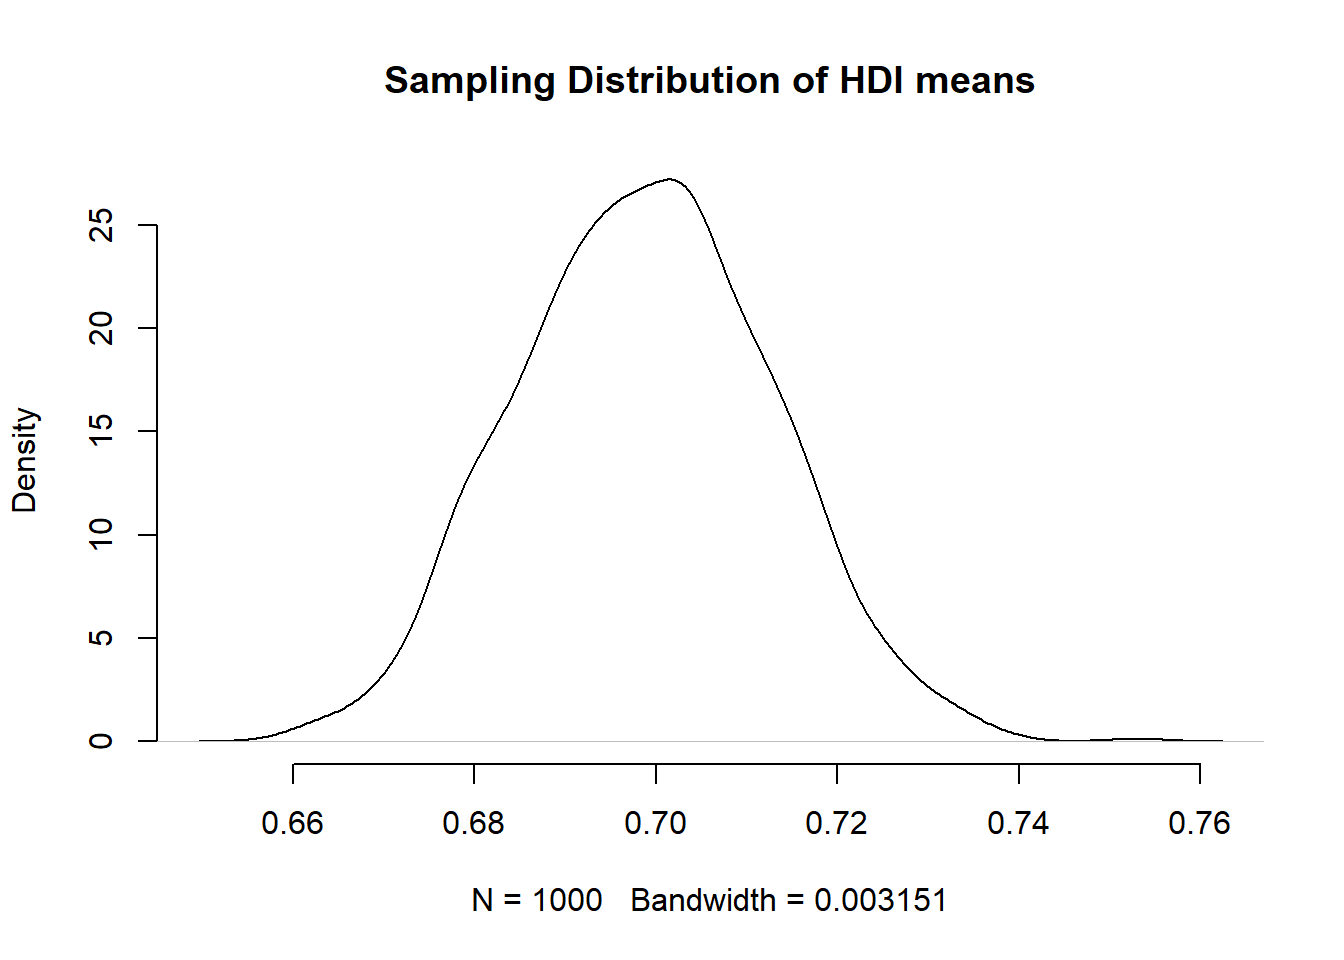
\includegraphics{statistics1_files/figure-latex/unnamed-chunk-130-1.pdf}

Beautiful Let's add the 95 percent confidence interval around our mean
estimate. The confidence interval quantifies our uncertainty. We said 95
percent of the time the mean would be in the interval from 0.6715367 to
0.7249432."

\begin{Shaded}
\begin{Highlighting}[]
\KeywordTok{abline}\NormalTok{( }\DataTypeTok{v =}\NormalTok{ lower.bound, }\DataTypeTok{lty =} \StringTok{"dashed"}\NormalTok{)}
\KeywordTok{abline}\NormalTok{( }\DataTypeTok{v =}\NormalTok{ upper.bound,  }\DataTypeTok{lty =} \StringTok{"dashed"}\NormalTok{)}
\end{Highlighting}
\end{Shaded}

You do not need to run the plot function again. You can just add to the
plot. Check the help function of \texttt{abline()} to see what its
arguments refer to.

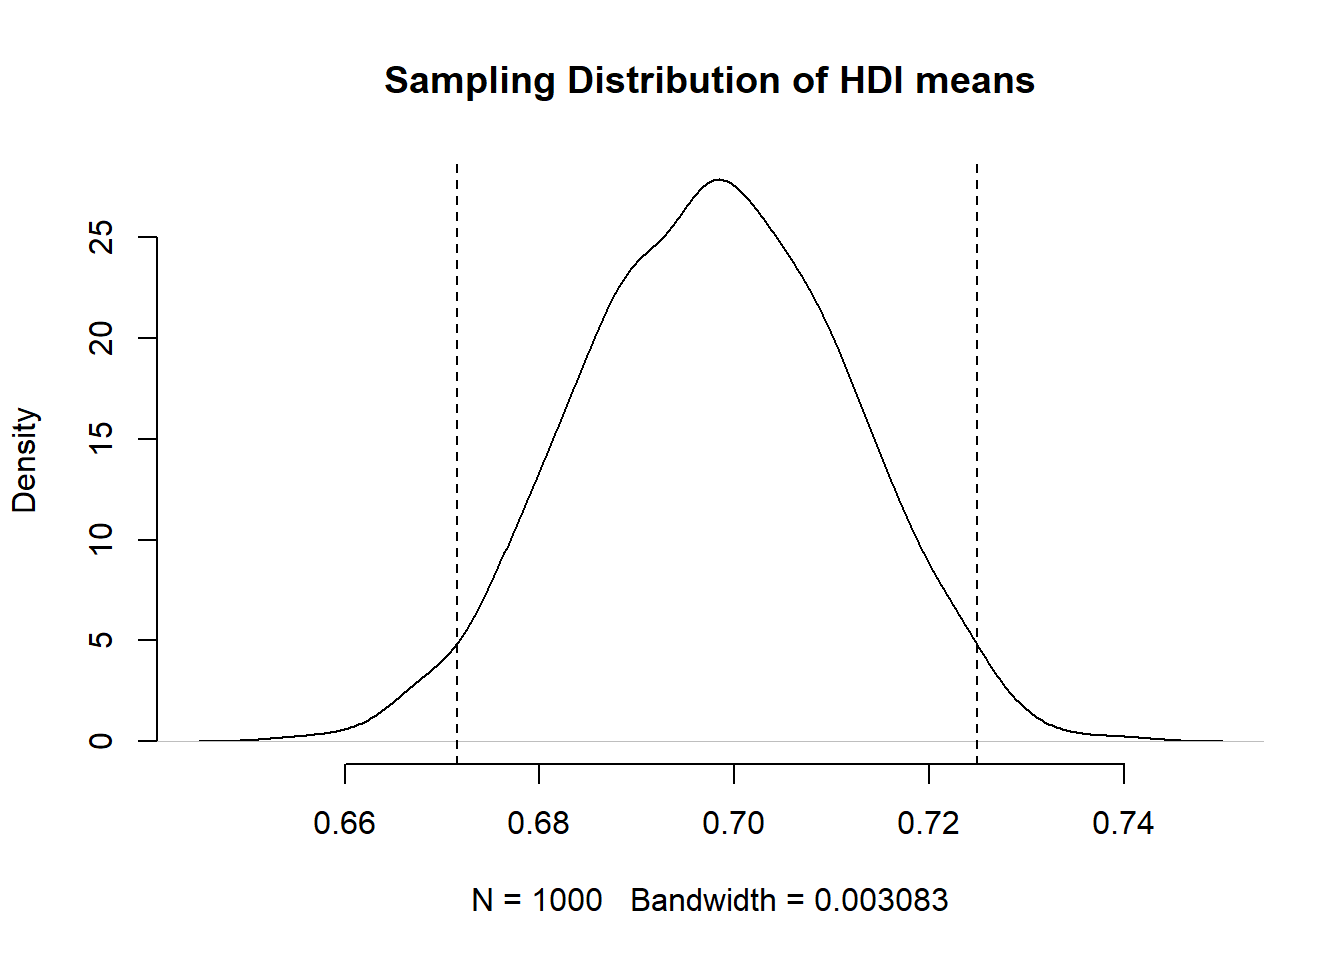
\includegraphics{statistics1_files/figure-latex/unnamed-chunk-132-1.pdf}

Fantastic! You can see that values below and above our confidence
interval are quite unlikely. Those values in the tails would not occur
often.

Not often, but not impossible.

Let's say that we wish know the probability that we take a sample and
our estimate of the mean is greater or equal 0.74. We would need to
integrate over the distribution from \(-\inf\) to 0.74. Fortunately R
has a function that does that for us. We need the \texttt{pnorm()}. It
calculates the probability of a value that is smaller or equal to the
value we specify. In other words, it gives us the probability from the
cumulative normal.

As the first argument \texttt{pnrom()} wants the value; 0.74 in our
case. The second and third arguments are the mean and the standard
deviation that characterise the normal distribution.

\begin{Shaded}
\begin{Highlighting}[]
\KeywordTok{pnorm}\NormalTok{(}\FloatTok{0.74}\NormalTok{, }\DataTypeTok{mean =}\NormalTok{ hdi.mean, }\DataTypeTok{sd =}\NormalTok{ se.hdi)}
\end{Highlighting}
\end{Shaded}

\begin{verbatim}
[1] 0.9989122
\end{verbatim}

What!? The probability to draw a mean 0.74 is 99.9 percent!? That cannot
be the value is so far in the tail of the distribution.

Well, this is the cumulative probability of drawing a value that is
equal to or smaller than 0.74. All probabilities sum to 1. So if we want
to know the probability of drawing a value that is greater than 0.74, we
subtract the probability, we just calculated, from 1.

\begin{Shaded}
\begin{Highlighting}[]
\DecValTok{1} \OperatorTok{-}\StringTok{ }\KeywordTok{pnorm}\NormalTok{(}\FloatTok{0.74}\NormalTok{, }\DataTypeTok{mean =}\NormalTok{ hdi.mean, }\DataTypeTok{sd =}\NormalTok{ se.hdi)}
\end{Highlighting}
\end{Shaded}

\begin{verbatim}
[1] 0.001087785
\end{verbatim}

Right, so the probability of getting a mean of \emph{hdi} in a sample is
0.1 percent.

\subsection{Conditional Distributions}\label{conditional-distributions}

Let's look at \emph{hdi} by \emph{former\_col}. The variable
\emph{former\_col} is 1 if a country is a former colony and 0 otherwise.
The variable \emph{hdi} is continuous.

Before we start, we plot the marginal pdf of \emph{hdi}.

\begin{Shaded}
\begin{Highlighting}[]
\KeywordTok{plot}\NormalTok{(}
  \KeywordTok{density}\NormalTok{(world.data}\OperatorTok{$}\NormalTok{hdi),}
  \DataTypeTok{bty =} \StringTok{"n"}\NormalTok{,}
  \DataTypeTok{main =} \StringTok{"Marginal Distribution of HDI"}
\NormalTok{)}
\end{Highlighting}
\end{Shaded}

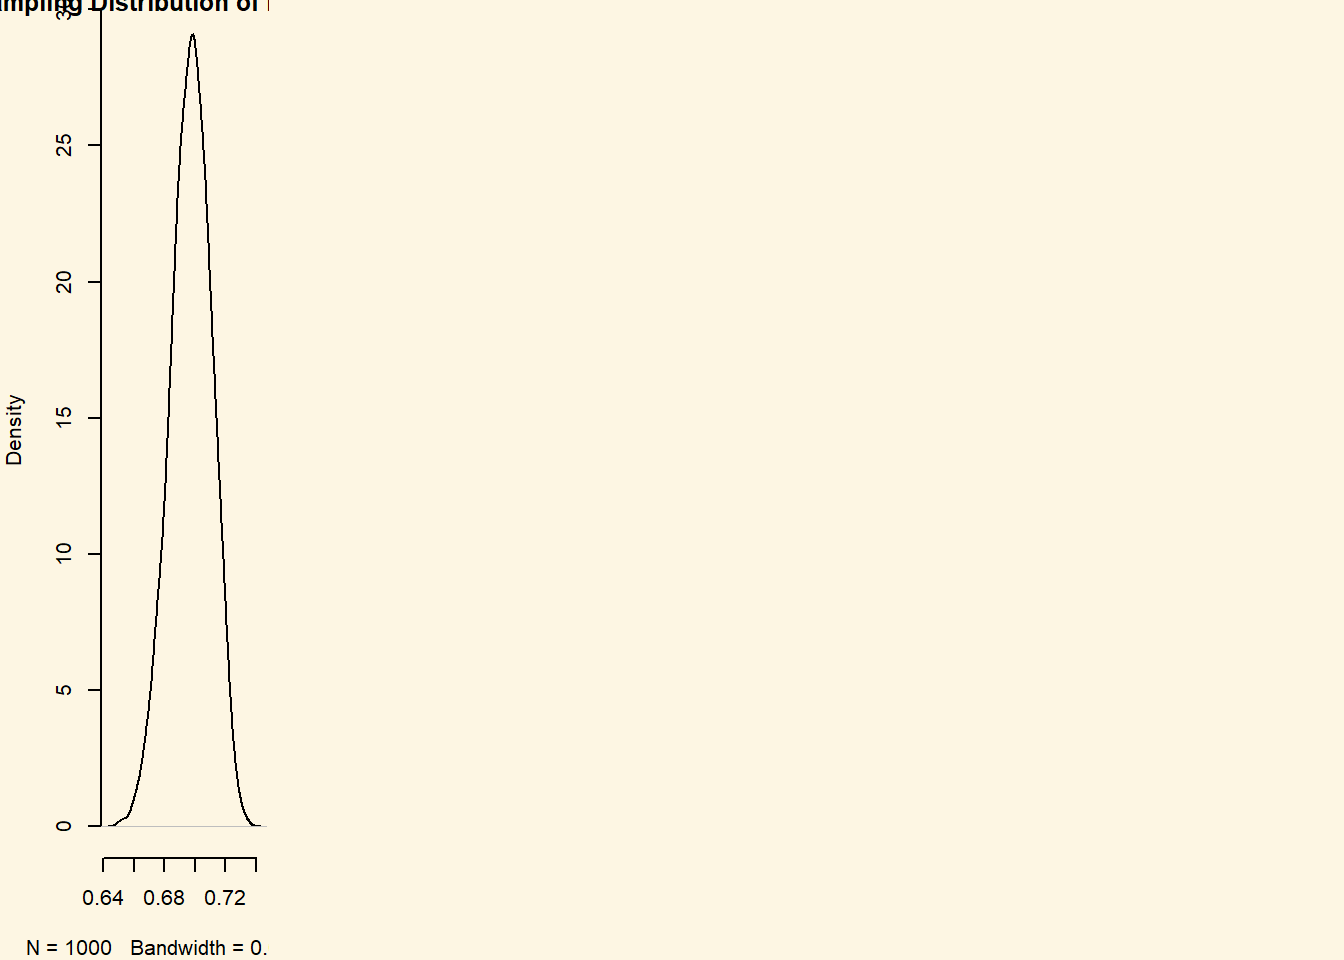
\includegraphics{statistics1_files/figure-latex/unnamed-chunk-135-1.pdf}

The distribution is bimodal. There is one peak at the higher development
end and one peak at the lower development end. Could it be that these
two peaks are conditional on whether a country was colonised or not?
Let's plot the conditional distributions.

\begin{Shaded}
\begin{Highlighting}[]
\KeywordTok{plot}\NormalTok{(}
  \KeywordTok{density}\NormalTok{(world.data}\OperatorTok{$}\NormalTok{hdi[world.data}\OperatorTok{$}\NormalTok{former_col }\OperatorTok{==}\StringTok{ }\DecValTok{0}\NormalTok{]),}
  \DataTypeTok{bty =} \StringTok{"n"}\NormalTok{,}
  \DataTypeTok{main =} \StringTok{"Conditional Distributions of HDI"}
\NormalTok{)}
\KeywordTok{lines}\NormalTok{(}\KeywordTok{density}\NormalTok{(world.data}\OperatorTok{$}\NormalTok{hdi), }\DataTypeTok{lty =} \StringTok{"dashed"}\NormalTok{)}
\KeywordTok{legend}\NormalTok{(}\StringTok{"topleft"}\NormalTok{, }\KeywordTok{c}\NormalTok{(}\StringTok{"not colonised"}\NormalTok{, }\StringTok{"colonised"}\NormalTok{), }\DataTypeTok{lty =} \KeywordTok{c}\NormalTok{(}\StringTok{"solid"}\NormalTok{, }\StringTok{"dashed"}\NormalTok{))}
\end{Highlighting}
\end{Shaded}

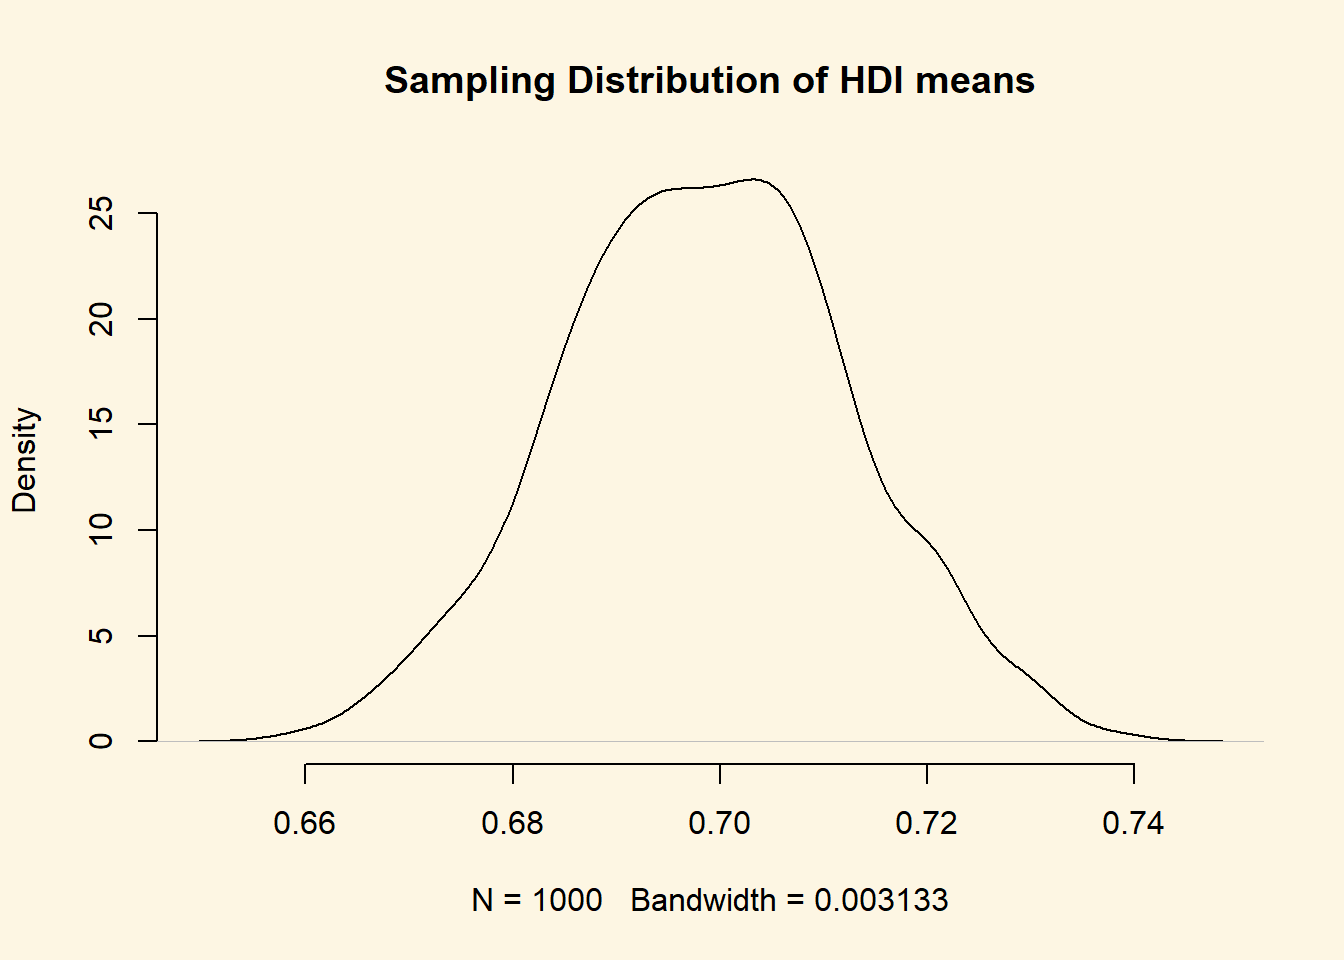
\includegraphics{statistics1_files/figure-latex/unnamed-chunk-136-1.pdf}

It's not quite like we expected. The distribution of human development
of not colonised countries is shifted to right of the distribution of
colonised countries and it is clearly narrower. Interestingly though,
the distribution of former colonies has a greater variance. Evidently,
some former colonies are doing very well and some are doing very poorly.
It seems like knowing whether a country was colonised or not tells us
something about its likely development but not enough. We cannot, e.g.,
say colonisation is the reason why countries do poorly. Probably, there
are differences among types of colonial institutions that were set up by
the colonisers.

Let's move on and examine the probability that a country has .8 or more
on \emph{hdi} given that it is a former colony.

We can get the cumulative probability with the \texttt{ecdf()} function.
It returns the empirical cumulative distribution, i.e., the cumulative
distribution of our data. We know that we can subset using square
brackets. That's all we need.

\begin{Shaded}
\begin{Highlighting}[]
\NormalTok{cumulative.p <-}\StringTok{ }\KeywordTok{ecdf}\NormalTok{(world.data}\OperatorTok{$}\NormalTok{hdi[ world.data}\OperatorTok{$}\NormalTok{former_col }\OperatorTok{==}\StringTok{ }\DecValTok{1}\NormalTok{ ])}
\DecValTok{1} \OperatorTok{-}\StringTok{ }\KeywordTok{cumulative.p}\NormalTok{(.}\DecValTok{8}\NormalTok{)}
\end{Highlighting}
\end{Shaded}

\begin{verbatim}
[1] 0.1666667
\end{verbatim}

Okay, the probability that a former colony has .8 or larger on the
\emph{hdi} is 16.6 percent. Go ahead figure out the probability for not
former colonies on your own.

\subsection{Exercises}\label{exercises-2}

\begin{enumerate}
\def\labelenumi{\arabic{enumi}.}
\tightlist
\item
  Create a script and call it assignment03. Save your script.
\item
  Load the \emph{world.data} dataset from your disk.
\item
  Rename the variable \emph{wdi\_gdpc} into \emph{gdpc}.
\item
  Delete missing values from \emph{gdpc}.
\item
  Inspect \emph{former\_col} and delete missing values from it.
\item
  Turn \emph{former\_col} into a factor variable with the appropriate
  lables.
\item
  Compute the probability that a county is richer than 55 000 per
  capita.
\item
  Compute the same probability given that a country is a former colony.
\item
  Compute the conditional expectation of wealth (gdp per capita) for a
  former colony.
\item
  Compute the conditional expectation of wealth for country that is not
  a former colony.
\item
  What is the probability that a former colony is 2 standard deviations
  below the mean wealth level?
\item
  What is the corresponding probability for a country that has not been
  colonised?
\item
  Compute the probability that a former colony is the wealth interval
  from 25 000 to 31 000.
\item
  Copmute the probability that a \textbf{not} former colony is in the
  top 2.5 percent of the wealth distribution.
\item
  At which wealth level is a country in the bottom 2.5 percent of the
  wealth distribution?
\end{enumerate}

\section{Solutions}\label{solutions-2}

\subsubsection{Exercise 2}\label{exercise-2-1}

Load the world.data dataset from your disk.

\begin{Shaded}
\begin{Highlighting}[]
\NormalTok{world.data <-}\StringTok{ }\KeywordTok{read.csv}\NormalTok{(}\StringTok{"QoG2012.csv"}\NormalTok{)}
\end{Highlighting}
\end{Shaded}

\subsubsection{Exercise 3}\label{exercise-3-2}

Rename the variable wdi\_gdpc into gdpc.

\begin{Shaded}
\begin{Highlighting}[]
\CommentTok{# to see all variable names}
\KeywordTok{names}\NormalTok{(world.data)}
\end{Highlighting}
\end{Shaded}

\begin{verbatim}
[1] "h_j"         "wdi_gdpc"    "undp_hdi"    "wbgi_cce"    "wbgi_pse"   
[6] "former_col"  "lp_lat_abst"
\end{verbatim}

\begin{Shaded}
\begin{Highlighting}[]
\CommentTok{# wdi_gdpc is the second variable. We rename the second element of the names vector}
\KeywordTok{names}\NormalTok{(world.data)[}\DecValTok{2}\NormalTok{] <-}\StringTok{ "gdpc"}
\end{Highlighting}
\end{Shaded}

\subsubsection{Exercise 4}\label{exercise-4-2}

Delete missing values from gdpc.

\begin{Shaded}
\begin{Highlighting}[]
\CommentTok{# to check whether there are any missings or not}
\KeywordTok{summary}\NormalTok{(world.data}\OperatorTok{$}\NormalTok{gdpc)}
\end{Highlighting}
\end{Shaded}

\begin{verbatim}
   Min. 1st Qu.  Median    Mean 3rd Qu.    Max.    NA's 
  226.2  1768.0  5326.1 10184.1 12976.5 63686.7      16 
\end{verbatim}

\begin{Shaded}
\begin{Highlighting}[]
\CommentTok{# we have missings, let's make a copy of world.data before deleting}
\NormalTok{full.world.data <-}\StringTok{ }\NormalTok{world.data}
\CommentTok{# now let's delete the 16 rows with missings on gdpc}
\NormalTok{world.data <-}\StringTok{ }\NormalTok{world.data[ }\KeywordTok{which}\NormalTok{(}\OperatorTok{!}\KeywordTok{is.na}\NormalTok{(world.data}\OperatorTok{$}\NormalTok{gdpc)) , ]}
\end{Highlighting}
\end{Shaded}

\subsubsection{Exercise 5}\label{exercise-5-2}

Inspect former\_col and delete missing values from it.

\begin{Shaded}
\begin{Highlighting}[]
\CommentTok{# we instpect the variable and check for missings}
\KeywordTok{summary}\NormalTok{(world.data}\OperatorTok{$}\NormalTok{former_col)}
\end{Highlighting}
\end{Shaded}

\begin{verbatim}
   Min. 1st Qu.  Median    Mean 3rd Qu.    Max. 
 0.0000  0.0000  1.0000  0.6348  1.0000  1.0000 
\end{verbatim}

\begin{Shaded}
\begin{Highlighting}[]
\CommentTok{# there are none, so there is nothing to delete}
\end{Highlighting}
\end{Shaded}

\subsubsection{Exercise 6}\label{exercise-6-2}

Turn former\_col into a factor variable with the appropriate labels.

\begin{Shaded}
\begin{Highlighting}[]
\CommentTok{# we check the current storage type}
\KeywordTok{str}\NormalTok{(world.data}\OperatorTok{$}\NormalTok{former_col)}
\end{Highlighting}
\end{Shaded}

\begin{verbatim}
 int [1:178] 0 0 1 1 1 0 1 0 0 1 ...
\end{verbatim}

\begin{Shaded}
\begin{Highlighting}[]
\CommentTok{# it's numeric, so we change it to nominal}
\NormalTok{world.data}\OperatorTok{$}\NormalTok{former_col <-}\StringTok{ }\KeywordTok{factor}\NormalTok{(world.data}\OperatorTok{$}\NormalTok{former_col, }
                                \DataTypeTok{levels =} \KeywordTok{c}\NormalTok{(}\DecValTok{0}\NormalTok{,}\DecValTok{1}\NormalTok{), }
                                \DataTypeTok{labels =} \KeywordTok{c}\NormalTok{(}\StringTok{"not colonised"}\NormalTok{, }\StringTok{"former colony"}\NormalTok{ ))}
\CommentTok{# let's check the results}
\KeywordTok{table}\NormalTok{(world.data}\OperatorTok{$}\NormalTok{former_col)}
\end{Highlighting}
\end{Shaded}

\begin{verbatim}

not colonised former colony 
           65           113 
\end{verbatim}

Wait a minute. Is there something wrong here? The mean of the variable
is 0.63. That means 63 percent of all countries are former colonies.
Let's check whether we got that.

\begin{Shaded}
\begin{Highlighting}[]
\KeywordTok{table}\NormalTok{(world.data}\OperatorTok{$}\NormalTok{former_col) }\OperatorTok{/}\StringTok{ }\KeywordTok{sum}\NormalTok{(}\KeywordTok{table}\NormalTok{(world.data}\OperatorTok{$}\NormalTok{former_col))}
\end{Highlighting}
\end{Shaded}

\begin{verbatim}

not colonised former colony 
    0.3651685     0.6348315 
\end{verbatim}

Ah, that's correct. It's good to make sure, we did not mess up the
re-coding.

\subsubsection{Exercise 8.}\label{exercise-8.}

Compute the probability that a county is richer than 55 000 per capita.

Wealth is never normally distributed. We don't even need to check. We
use the \texttt{ecdf()} function for the empirical cumulative
distribution.

The probability that a country is richer than 55 000 is 1 minus the
cumulative probability of 55000.

\begin{Shaded}
\begin{Highlighting}[]
\CommentTok{# get the empirical cumulative distribution of wealth}
\NormalTok{c.dist.of.wealth <-}\StringTok{ }\KeywordTok{ecdf}\NormalTok{(world.data}\OperatorTok{$}\NormalTok{gdpc)}
\CommentTok{# the prob}
\DecValTok{1} \OperatorTok{-}\StringTok{ }\KeywordTok{c.dist.of.wealth}\NormalTok{(}\DecValTok{55000}\NormalTok{)}
\end{Highlighting}
\end{Shaded}

\begin{verbatim}
[1] 0.01123596
\end{verbatim}

The probability is 0.01. Put differently 1 percent of countries is
richer than 55 000 US dollars per capita.

\subsubsection{Exercise 8}\label{exercise-8-2}

Compute the same probability given that a country is a former colony.

The approach is similar but we want the conditional cumulative
distribution, where the condition is that a country is a former colony.

\begin{Shaded}
\begin{Highlighting}[]
\CommentTok{# conditional cumulative distribution}
\NormalTok{c.dist.of.wealth2 <-}\StringTok{ }\KeywordTok{ecdf}\NormalTok{(world.data}\OperatorTok{$}\NormalTok{gdpc[world.data}\OperatorTok{$}\NormalTok{former_col }\OperatorTok{==}\StringTok{ "former colony"}\NormalTok{])}
\DecValTok{1} \OperatorTok{-}\StringTok{ }\KeywordTok{c.dist.of.wealth2}\NormalTok{(}\DecValTok{55000}\NormalTok{)}
\end{Highlighting}
\end{Shaded}

\begin{verbatim}
[1] 0.008849558
\end{verbatim}

The probability is 0.009. The probability that a former colony is that
rich is slightly lower than that any country is.

\subsubsection{Exercise 9}\label{exercise-9-1}

Compute the conditional expectation of wealth (gdp per capita) for a
former colony.

The conditional expectation is the mean of wealth among all former
colonies. We know how to do this from last week. We take the mean of
wealth and subset using square brackets.

\begin{Shaded}
\begin{Highlighting}[]
\KeywordTok{mean}\NormalTok{( world.data}\OperatorTok{$}\NormalTok{gdpc[world.data}\OperatorTok{$}\NormalTok{former_col }\OperatorTok{==}\StringTok{ "former colony"}\NormalTok{] )}
\end{Highlighting}
\end{Shaded}

\begin{verbatim}
[1] 6599.714
\end{verbatim}

The conditional expectation of wealth for former colonies is 6600 US
dollars per capita.

\subsubsection{Exercise 10}\label{exercise-10-1}

Compute the conditional expectation of wealth for a country that is not
a former colony.

\begin{Shaded}
\begin{Highlighting}[]
\KeywordTok{mean}\NormalTok{( world.data}\OperatorTok{$}\NormalTok{gdpc[world.data}\OperatorTok{$}\NormalTok{former_col }\OperatorTok{==}\StringTok{ "not colonised"}\NormalTok{] )}
\end{Highlighting}
\end{Shaded}

\begin{verbatim}
[1] 16415.39
\end{verbatim}

The corresponding expectation for countries that have not been a colony
is 16415 US dollars.

\subsubsection{Exercise 11}\label{exercise-11}

What is the probability that a former colony is 2 standard deviations
below the mean wealth level?

We first find out what a standard deviation of wealth is in the
conditional distribution of wealth for former colonies.

\begin{Shaded}
\begin{Highlighting}[]
\CommentTok{# standard deviation of wealth for former colonies}
\NormalTok{sd.wealth.cols <-}\StringTok{ }\KeywordTok{sd}\NormalTok{(world.data}\OperatorTok{$}\NormalTok{gdpc[world.data}\OperatorTok{$}\NormalTok{former_col }\OperatorTok{==}\StringTok{ "former colony"}\NormalTok{])}
\NormalTok{sd.wealth.cols}
\end{Highlighting}
\end{Shaded}

\begin{verbatim}
[1] 9783.914
\end{verbatim}

Interesting, the standard deviation is greater than the mean.
Apparently, former colonies are very different. Some do poorly and some
extremely well.

Doesn't this pose a problem for the task though? How can a country's
wealth be 2 standard deviations below the mean if the mean is smaller
than the standard deviation?

Well, that's not possible. Negative wealth does not exist. Consequently,
that probability is 0.

\subsubsection{Exercise 12}\label{exercise-12}

We get the standard deviation of the wealth distribution of countries
that have not been colonised.

\begin{Shaded}
\begin{Highlighting}[]
\CommentTok{# standard deviation of wealth for not former colonies}
\NormalTok{sd.wealth.not.cols <-}\StringTok{ }\KeywordTok{sd}\NormalTok{(world.data}\OperatorTok{$}\NormalTok{gdpc[world.data}\OperatorTok{$}\NormalTok{former_col }\OperatorTok{==}\StringTok{ "not colonised"}\NormalTok{])}
\end{Highlighting}
\end{Shaded}

The result is similar to exercise 11. The mean is 16 415 and the
standard deviation is 13 766. 2 standard deviations below the mean would
be negative. The probability of that is 0.

\subsubsection{Exercise 13}\label{exercise-13}

Compute the probability that a former colony is the wealth interval from
25 000 to 31 000.

We compute the cumulative probabilities that a country has 31 000 and 25
000 and then take the difference.

\begin{Shaded}
\begin{Highlighting}[]
\CommentTok{# cumulative probability of 31 000}
\NormalTok{p1 <-}\StringTok{ }\KeywordTok{c.dist.of.wealth2}\NormalTok{(}\DecValTok{31000}\NormalTok{)}
\CommentTok{# cumulative probability of 25 000}
\NormalTok{p2 <-}\StringTok{ }\KeywordTok{c.dist.of.wealth2}\NormalTok{(}\DecValTok{25000}\NormalTok{)}
\CommentTok{# probability of country in the interval}
\NormalTok{p1 }\OperatorTok{-}\StringTok{ }\NormalTok{p2}
\end{Highlighting}
\end{Shaded}

\begin{verbatim}
[1] 0
\end{verbatim}

The answer is again: 0. Let's have a look at the distribution to see
what's going on there.

\begin{Shaded}
\begin{Highlighting}[]
\KeywordTok{plot}\NormalTok{(}\KeywordTok{density}\NormalTok{( world.data}\OperatorTok{$}\NormalTok{gdpc[world.data}\OperatorTok{$}\NormalTok{former_col }\OperatorTok{==}\StringTok{ "former colony"}\NormalTok{] ))}
\end{Highlighting}
\end{Shaded}

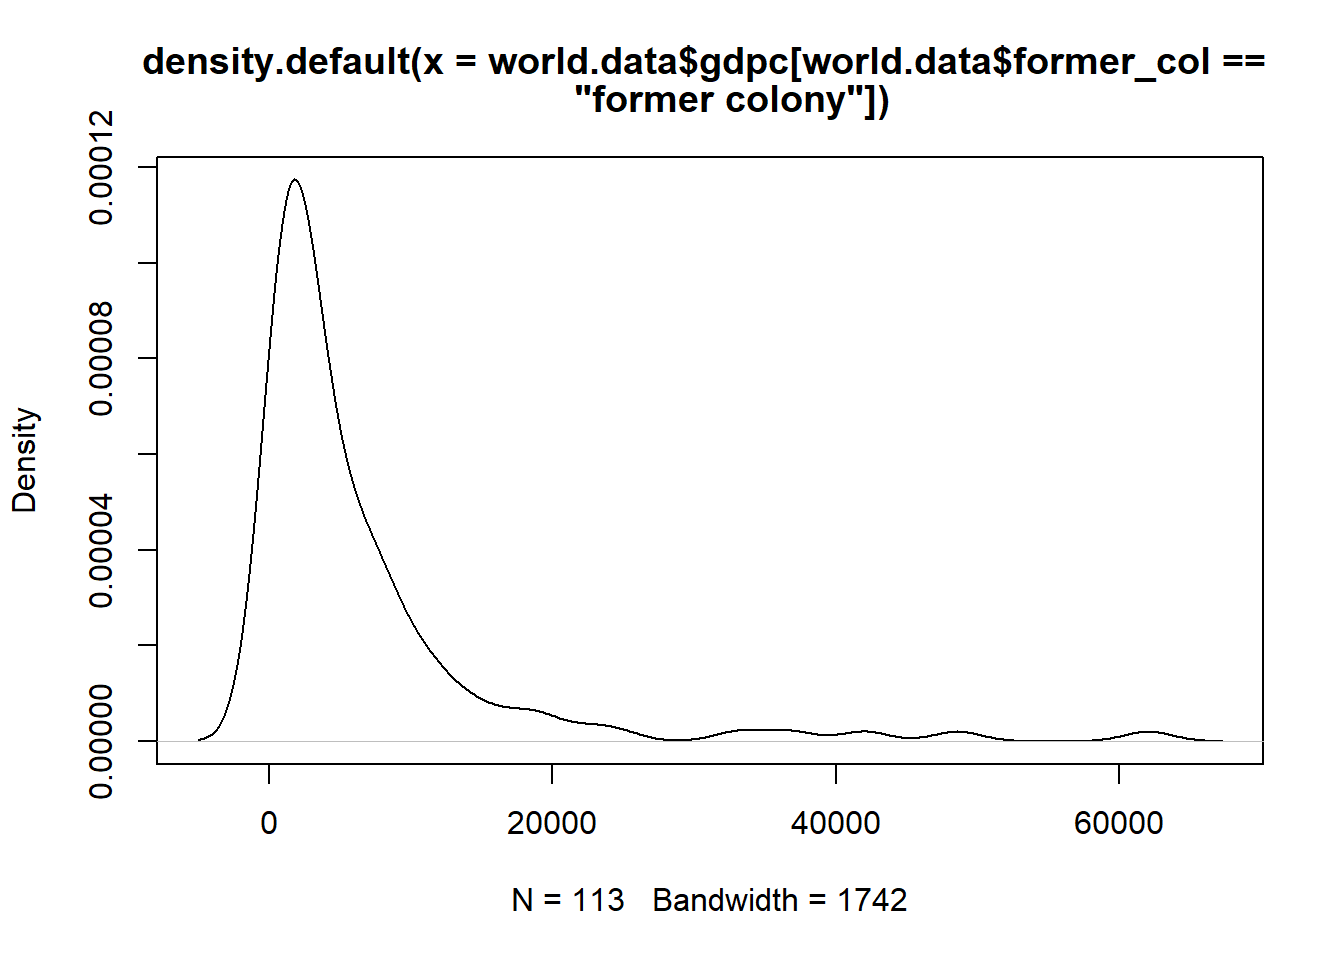
\includegraphics{statistics1_files/figure-latex/unnamed-chunk-152-1.pdf}

It seems like there are no countries in that interval. Let's check:

\begin{Shaded}
\begin{Highlighting}[]
\CommentTok{# let's look at summary stats first}
\KeywordTok{summary}\NormalTok{(world.data}\OperatorTok{$}\NormalTok{gdpc[ world.data}\OperatorTok{$}\NormalTok{former_col }\OperatorTok{==}\StringTok{ "former colony"}\NormalTok{  ])}
\end{Highlighting}
\end{Shaded}

\begin{verbatim}
   Min. 1st Qu.  Median    Mean 3rd Qu.    Max. 
  226.2  1263.7  3157.5  6599.7  7938.3 62005.6 
\end{verbatim}

\begin{Shaded}
\begin{Highlighting}[]
\CommentTok{# so there is at least 1 country that is richer. Let's look at all }
\CommentTok{# countries that are former colonies and also richer than 25 000}
\NormalTok{world.data[}\KeywordTok{which}\NormalTok{( world.data}\OperatorTok{$}\NormalTok{gdpc }\OperatorTok{>}\StringTok{ }\DecValTok{25000} \OperatorTok{&}\StringTok{ }\NormalTok{world.data}\OperatorTok{$}\NormalTok{former_col }\OperatorTok{==}\StringTok{ "former colony"}\NormalTok{), ]}
\end{Highlighting}
\end{Shaded}

\begin{verbatim}
    h_j     gdpc undp_hdi  wbgi_cce    wbgi_pse    former_col lp_lat_abst
24    0 48585.73    0.867 0.3304393  0.99980551 former colony   0.0477778
92    1 33079.87    0.838 1.0835209 -0.02684768 former colony   0.3255555
142   0 62005.56    0.833 0.9734111  0.76874268 former colony   0.2811111
156   1 36732.23    0.902 2.3715818  1.34370053 former colony   0.0135556
175   0 42004.04    0.824 1.0449655  0.80680293 former colony   0.2666667
\end{verbatim}

That's it. There are exactly zero countries in that interval.

Sub-setting with 2 conditions in square brackets may be new to you. We
did that with \texttt{\&} operator which means ``and''.

\subsubsection{Exercise 14}\label{exercise-14}

Compute the probability that a not former colony is in the top 2.5
percent of the wealth distribution.

We find the value first. The top 2.5 percent are in the 97.5 percentile
of the distribution. We use the \texttt{quantile()} function to get the
value of the 97.5th percentile.

\begin{Shaded}
\begin{Highlighting}[]
\NormalTok{rich.countries <-}\StringTok{ }\KeywordTok{quantile}\NormalTok{(world.data}\OperatorTok{$}\NormalTok{gdpc[ world.data}\OperatorTok{$}\NormalTok{former_col }\OperatorTok{==}\StringTok{ "not colonised"}\NormalTok{], .}\DecValTok{975}\NormalTok{)}
\NormalTok{rich.countries}
\end{Highlighting}
\end{Shaded}

\begin{verbatim}
   97.5% 
41447.31 
\end{verbatim}

The value that puts a country in the top 2.5 percent of the conditional
wealth distribution (where the condition is that a country was not
colonised) is 41447 US dollars.

We now take the empirical cumulative distribution and get the
probability of being richer.

\begin{Shaded}
\begin{Highlighting}[]
\CommentTok{# conditional cumulative distribution}
\NormalTok{c.dist.of.wealth3 <-}\StringTok{ }\KeywordTok{ecdf}\NormalTok{(world.data}\OperatorTok{$}\NormalTok{gdpc[world.data}\OperatorTok{$}\NormalTok{former_col }\OperatorTok{==}\StringTok{ "not colonised"}\NormalTok{])}
\CommentTok{# conditional probability of being in the top 2.5 percent of not colonised countries}
\DecValTok{1} \OperatorTok{-}\StringTok{ }\KeywordTok{c.dist.of.wealth3}\NormalTok{(rich.countries)}
\end{Highlighting}
\end{Shaded}

\begin{verbatim}
[1] 0.03076923
\end{verbatim}

The probability is 0.03.

\subsubsection{Exercise 15}\label{exercise-15}

At which wealth level is a country in the bottom 2.5 percent of the
wealth distribution?

The question asks for the wealth level that puts a country in the bottom
2.5 percent independent of whether it was a colony or not. The
\texttt{quantile()} function returns that value.

\begin{Shaded}
\begin{Highlighting}[]
\KeywordTok{quantile}\NormalTok{( world.data}\OperatorTok{$}\NormalTok{gdpc, .}\DecValTok{025}\NormalTok{ )}
\end{Highlighting}
\end{Shaded}

\begin{verbatim}
    2.5% 
526.8697 
\end{verbatim}

At 527 US dollars per capita, a country is in the bottom 2.5 percent of
the wealth distribution.

\chapter{T-test for Difference in Means and Hypothesis
Testing}\label{t-test-for-difference-in-means-and-hypothesis-testing}

\section{Seminar}\label{seminar-3}

Let's remove all objects from our workspace and set the working
directory.

\begin{Shaded}
\begin{Highlighting}[]
\KeywordTok{rm}\NormalTok{(}\DataTypeTok{list=}\KeywordTok{ls}\NormalTok{())}
\KeywordTok{setwd}\NormalTok{(}\StringTok{"~/statistics1"}\NormalTok{)}
\end{Highlighting}
\end{Shaded}

We load the data from the \href{http://qog.pol.gu.se/}{Quality of
Government Institute} again. Let's have a look at the codebook:

\begin{tabular}{l|l}
\hline
Variable & Description\\
\hline
h\_j & 1 if Free Judiciary\\
\hline
wdi\_gdpc & Per capita wealth in US dollars\\
\hline
undp\_hdi & Human development index (higher values = higher quality of life)\\
\hline
wbgi\_cce & Control of corruption index (higher values = more control of corruption)\\
\hline
wbgi\_pse & Political stability index (higher values = more stable)\\
\hline
former\_col & 1 = country was a colony once\\
\hline
lp\_lat\_abst & Latitude of country's captial divided by 90\\
\hline
\end{tabular}

Let's load the data.

\begin{Shaded}
\begin{Highlighting}[]
\NormalTok{world.data <-}\StringTok{ }\KeywordTok{read.csv}\NormalTok{(}\StringTok{"QoG2012.csv"}\NormalTok{)}
\end{Highlighting}
\end{Shaded}

We can get summary statistics of each variable in the dataset by using
the \texttt{summary()} function over the dataset.

\begin{Shaded}
\begin{Highlighting}[]
\KeywordTok{summary}\NormalTok{(world.data)}
\end{Highlighting}
\end{Shaded}

\begin{verbatim}
      h_j            wdi_gdpc          undp_hdi         wbgi_cce       
 Min.   :0.0000   Min.   :  226.2   Min.   :0.2730   Min.   :-1.69953  
 1st Qu.:0.0000   1st Qu.: 1768.0   1st Qu.:0.5390   1st Qu.:-0.81965  
 Median :0.0000   Median : 5326.1   Median :0.7510   Median :-0.30476  
 Mean   :0.3787   Mean   :10184.1   Mean   :0.6982   Mean   :-0.05072  
 3rd Qu.:1.0000   3rd Qu.:12976.5   3rd Qu.:0.8335   3rd Qu.: 0.50649  
 Max.   :1.0000   Max.   :63686.7   Max.   :0.9560   Max.   : 2.44565  
 NA's   :25       NA's   :16        NA's   :19       NA's   :2         
    wbgi_pse          former_col      lp_lat_abst    
 Min.   :-2.46746   Min.   :0.0000   Min.   :0.0000  
 1st Qu.:-0.72900   1st Qu.:0.0000   1st Qu.:0.1343  
 Median : 0.02772   Median :1.0000   Median :0.2444  
 Mean   :-0.03957   Mean   :0.6289   Mean   :0.2829  
 3rd Qu.: 0.79847   3rd Qu.:1.0000   3rd Qu.:0.4444  
 Max.   : 1.67561   Max.   :1.0000   Max.   :0.7222  
                                     NA's   :7       
\end{verbatim}

\subsection{The Standard Error}\label{the-standard-error}

The standard error of an estimate quantifies uncertainty that is due to
sampling variability. Recall that we infer from a sample to the
population. Let's have a look at \emph{wdi\_gdpc} which is gdp per
capita. We re-name the variable to \emph{wealth}.

\begin{Shaded}
\begin{Highlighting}[]
\KeywordTok{names}\NormalTok{(world.data)[}\DecValTok{2}\NormalTok{] <-}\StringTok{ "wealth"} 
\KeywordTok{names}\NormalTok{(world.data)}
\end{Highlighting}
\end{Shaded}

\begin{verbatim}
[1] "h_j"         "wealth"      "undp_hdi"    "wbgi_cce"    "wbgi_pse"   
[6] "former_col"  "lp_lat_abst"
\end{verbatim}

Let's look at the mean.

\begin{Shaded}
\begin{Highlighting}[]
\KeywordTok{mean}\NormalTok{(world.data}\OperatorTok{$}\NormalTok{wealth)}
\end{Highlighting}
\end{Shaded}

\begin{verbatim}
[1] NA
\end{verbatim}

R returns NA because there are missing values on the \emph{wealth}
variable and we cannot calculate with NAs. For instance,
\texttt{2\ +\ NA} will return NA. We make a copy of the full data set
and then delete missing values.

\begin{Shaded}
\begin{Highlighting}[]
\CommentTok{# copy of the dataset}
\NormalTok{full.data <-}\StringTok{ }\NormalTok{world.data}

\CommentTok{# delete rows from dataset that have missings on wealth variable}
\NormalTok{world.data <-}\StringTok{ }\NormalTok{world.data[ }\OperatorTok{!}\KeywordTok{is.na}\NormalTok{(world.data}\OperatorTok{$}\NormalTok{wealth) , ]}
\end{Highlighting}
\end{Shaded}

Now, we compute the mean again.

\begin{Shaded}
\begin{Highlighting}[]
\KeywordTok{mean}\NormalTok{(world.data}\OperatorTok{$}\NormalTok{wealth)}
\end{Highlighting}
\end{Shaded}

\begin{verbatim}
[1] 10184.09
\end{verbatim}

The mean estimate in our sample is \textasciitilde{}10184.09. We are
generally interested in the population. Therefore, we infer from our
sample to the population. Our main problem is that samples are subject
to sampling variability. If we take another sample, our mean estimate
would be different. The standard error quantifies this type of
uncertainty.

The formula for the standard error of the mean is:
\[ SE(\bar{Y}) = \frac{s_Y}{\sqrt{n}}  \]

Where \(s_Y\) is the standard deviation (of \emph{wealth}) and \(n\) is
the number of observations in (of \emph{wealth}).

We compute the standard error in R:

\begin{Shaded}
\begin{Highlighting}[]
\NormalTok{se.y_bar <-}\StringTok{ }\NormalTok{(}\KeywordTok{sd}\NormalTok{(world.data}\OperatorTok{$}\NormalTok{wealth) }\OperatorTok{/}\StringTok{ }\KeywordTok{sqrt}\NormalTok{( }\KeywordTok{length}\NormalTok{(world.data}\OperatorTok{$}\NormalTok{wealth) ))}
\end{Highlighting}
\end{Shaded}

The standard error is \textasciitilde{}922.73. The mean of the sampling
distribution (recall that we get a sampling distribution if we sample
repeatedly) is the population mean. The standard error is the average
difference from the population mean. That means, if we take 1 sample (as
we have), the average deviation in the mean estimate from the population
mean is equal to the standard error.

We need the standard error for hypothesis testing. You will see how in
the following.

\subsection{T-test (one sample hypothesis
test)}\label{t-test-one-sample-hypothesis-test}

A knowledgeable friend declares that worldwide wealth stands at exactly
10 000 US dollars per capita today. We would like to know whether she is
right and tease her relentlessly if she isn't.

So, first we take the mean of the \emph{wealth} variable.

\begin{Shaded}
\begin{Highlighting}[]
\KeywordTok{mean}\NormalTok{(world.data}\OperatorTok{$}\NormalTok{wealth)}
\end{Highlighting}
\end{Shaded}

\begin{verbatim}
[1] 10184.09
\end{verbatim}

Wow, our friend is quite close. Substantially, the difference of our
friends claim to our estimate is small but we could still find that the
difference is statistically significant (it's a noticeable systematic
difference).

Because we do not have information on all countries, our 10184.09 is an
estimate and the true population mean -- the population here would be
all countries in the world -- may be 10000 as our friend claims. We test
this statistically.

In statistics jargon: we would like to test whether our estimate is
statistically different from the 10000 figure (the null hypothesis)
suggested by our friend. Put differently, we would like to know the
probability that we estimate 10184.09 if the true mean of all countries
is 10000.

Recall, that the standard error of the mean (which is the estimate of
the true standard deviation of the population mean) is estimated as:

\[ \frac{s_{Y}}{\sqrt{n}} \]

Before we estimate the standard error, let's get \(n\) (the number of
observations). We have done this above but to make our code more
readable, we save the number of observations in an object that we call
\texttt{n}.

\begin{Shaded}
\begin{Highlighting}[]
\NormalTok{n <-}\StringTok{ }\KeywordTok{length}\NormalTok{(world.data}\OperatorTok{$}\NormalTok{wealth)}
\NormalTok{n}
\end{Highlighting}
\end{Shaded}

\begin{verbatim}
[1] 178
\end{verbatim}

With the function \texttt{length(world.data\$world)} we get all
observations in the data. Now, let's take the standard error of the mean
again.

\begin{Shaded}
\begin{Highlighting}[]
\NormalTok{se.y_bar <-}\StringTok{ }\KeywordTok{sd}\NormalTok{(world.data}\OperatorTok{$}\NormalTok{wealth) }\OperatorTok{/}\StringTok{ }\KeywordTok{sqrt}\NormalTok{(n)}
\end{Highlighting}
\end{Shaded}

We know that 1 standard error is one average deviation from the
population mean. The sampling distribution is approximately normal. 95
percent of the observations under the normal distribution are within 2
standard deviations of the mean.

We construct the confidence interval within which the population mean
lies with 95 percent probability in the following way. First, we take
our mean estimate of \emph{wealth}. That's the sample mean and not the
population mean. Second, we go 2 standard errors to the left of it. This
is the lower bound of our confidence interval. Third, we go 2 standard
deviations to the right of the sample mean. That is the upper bound of
our confidence interval.

The 95 percent confidence interval around the sample means gives the
interval within which the population mean lies with 95 percent
probability.

We want to know what the population mean is, right? Yes, that's right.
Therefore, we want the confidence interval to be as narrow as possible.
The narrower the confidence interval, the more precise we are about what
the population mean is like. For instance, saying the population mean of
income is between 9 950 and 10 050 is more precise than saying the
population mean is between 5 000 and 15 000.

We construct the confidence interval with the standard error. That
means, the smaller the standard error, the more precise our estimate.
The formula for the confidence interval is:

\[ \bar{Y} \pm 1.96 \times SE(\bar{Y}) \]

``Where does the 1.96 come from'', you ask. It's a critical value. More
on that later. For now, just recall that in a normal distribution 95
percent of all observations are within 1.96 standard errors of the mean.

We now construct our confidence interval. Our sample is large enough to
assume that the sampling distribution is approximately normal. So, we
can go \(1.96\) standard deviations to the left and to the right of the
mean to construct our \(95\%\) confidence interval.

\begin{Shaded}
\begin{Highlighting}[]
\CommentTok{# lower bound}
\NormalTok{lb <-}\StringTok{ }\KeywordTok{mean}\NormalTok{(world.data}\OperatorTok{$}\NormalTok{wealth) }\OperatorTok{-}\StringTok{ }\FloatTok{1.96} \OperatorTok{*}\StringTok{ }\NormalTok{se.y_bar}
\CommentTok{# upper bound}
\NormalTok{ub <-}\StringTok{ }\KeywordTok{mean}\NormalTok{(world.data}\OperatorTok{$}\NormalTok{wealth) }\OperatorTok{+}\StringTok{ }\FloatTok{1.96} \OperatorTok{*}\StringTok{ }\NormalTok{se.y_bar}
\CommentTok{# results (the population mean lies within this interval with 95% probability)}
\NormalTok{lb }\CommentTok{# lower bound}
\end{Highlighting}
\end{Shaded}

\begin{verbatim}
[1] 8375.531
\end{verbatim}

\begin{Shaded}
\begin{Highlighting}[]
\KeywordTok{mean}\NormalTok{(world.data}\OperatorTok{$}\NormalTok{wealth) }\CommentTok{# sample mean}
\end{Highlighting}
\end{Shaded}

\begin{verbatim}
[1] 10184.09
\end{verbatim}

\begin{Shaded}
\begin{Highlighting}[]
\NormalTok{ub }\CommentTok{# upper bound}
\end{Highlighting}
\end{Shaded}

\begin{verbatim}
[1] 11992.65
\end{verbatim}

So we are \(95\%\) confident that the population average level of wealth
is between 8375.53 US dollars and 11992.65 US dollars. You can see that
we are not very certain about our estimate and we most definitely cannot
rule out that our friend is right (she claimed that the population mean
is 10 0000---that is within our interval. Hence, we cannot reject it).

A different way of describing our finding is to emphasize the logic of
(hypothetical) repeated sampling. In a process of repeated sampling we
can expect that the confidence interval that we calculate for each
sample will include the true population value \(95\%\) of the time. That
is equivalent to what we said earlier because a probability is the
long-run relative frequency of an outcome.

\subsubsection{The t value}\label{the-t-value}

We now estimate the t value. Recall that our friend claimed that the
population mean was 10 000. This is the null hypothesis that we wish to
falsify. We estimated something else in our data, namely 10184.0910395.
The t value is the difference between our estimate (the result we get by
looking at data) and the population mean under the null hypothesis
divided by the standard error of the mean.

\[ \frac{ \bar{Y} - \mu_0 } {SE(\bar{Y})} \]

Where \(\bar{Y}\) is the mean in our data, \(\mu_0\) is the population
mean under the null hypothesis and \(SE(\bar{Y})\) is the standard error
of the mean.

Okay, let's compute this in R:

\begin{Shaded}
\begin{Highlighting}[]
\NormalTok{t.value <-}\StringTok{ }\NormalTok{(}\KeywordTok{mean}\NormalTok{(world.data}\OperatorTok{$}\NormalTok{wealth) }\OperatorTok{-}\StringTok{ }\DecValTok{10000}\NormalTok{) }\OperatorTok{/}\StringTok{ }\NormalTok{se.y_bar}
\NormalTok{t.value}
\end{Highlighting}
\end{Shaded}

\begin{verbatim}
[1] 0.1995059
\end{verbatim}

Look at the formula until you understand what is going on. In the
numerator we take the difference between our estimate and the population
mean under the null hypothesis. In expectation that difference should be
0 assuming that the null hypothesis is true. The larger that difference,
the less likely that the null hypothesis is true.

We divide by the standard error to transform the units of the difference
into standard deviations. Before our difference was in the units of
whatever variable we are looking at (US dollars in our example). By
dividing by the standard error, we have normed the variable. It is now
in standard deviations from the mean.

Assume that the null hypothesis is true. In expectation the difference
between our estimate in the data and the population mean should be
\textbf{0 standard deviations}. The more standard deviations our
estimate is away from the population mean under the null hypothesis, the
less likely it is that the null hypothesis is true.

Within \textbf{1.96 standard deviations} from the mean lie 95 percent of
all observations. That means that if the difference that we estimated is
further than 1.96 standard deviations from the mean, it is very unlikely
that the null hypothesis is true. ``How unlikely,'' you ask. Well that
is the p value. If our estimated difference is more than 1.96 standard
deviations from the mean, then the probability that the null hypothesis
is true, is less than 5 percent.

Back to our t value. We estimated a t value of 0.1995059. That means
that a sample estimate of \texttt{mean(world.data\$wealth)} is 0.1995059
standard deviations from the population mean under the null hypothesis
(10 000 in our sample).

Our t value suggests that if the null hypothesis were true, our sample
estimate would only be 0.1995059 standard deviations away from the
population mean under the null. That is not at all unlikely. We can only
reject the null hypothesis if we are more than 1.96 standard deviations
away from the mean.

\subsubsection{The p value}\label{the-p-value}

Let's estimate the precise p-value by calculating how likely it would be
to observe a t-statistic of 0.1995059 from a t-distribution with n - 1
(177) degrees of freedom.

The function \texttt{pt(t.value,\ df\ =\ n-1)} is the cumulative
probability that we get the t.value we put into the formula if the null
is true. The cumulative probability is estimated as the interval from
minus infinity to our t.value. So, 1 minus that probability is the
probability that we see anything larger (in the right tale of the
distribution). But we are testing whether the true mean is different
from 10000 (including smaller). Therefore, we want the probability that
we see a t.value in the right tale \emph{or} in the left tale of the
distribution. The distribution is symmetric. So we can just calculate
the probability of seeing a t-value in the right tale and multiply it by
2.

\begin{Shaded}
\begin{Highlighting}[]
\DecValTok{2}\OperatorTok{*}\StringTok{ }\NormalTok{( }\DecValTok{1} \OperatorTok{-}\StringTok{ }\KeywordTok{pt}\NormalTok{(t.value, }\DataTypeTok{df =}\NormalTok{ (n}\OperatorTok{-}\DecValTok{1}\NormalTok{) ))}
\end{Highlighting}
\end{Shaded}

\begin{verbatim}
[1] 0.8420961
\end{verbatim}

The p-value is way too large to reject the null hypothesis (the true
population mean is 10 000). If we specified an alpha-level of 0.05 in
advance, we would reject it only if the p-value was smaller than 0.05.
If we specified an alpha-level of 0.01 in advance, we would reject it
only if the p-value was smaller than 0.01, and so on.

Let's verify this using the the t-test function \texttt{t.test()}. The
syntax of the function is:

\begin{verbatim}
t.test(formula, mu, alt, conf)
\end{verbatim}

Lets have a look at the arguments.

\begin{longtable}[]{@{}ll@{}}
\toprule
\begin{minipage}[b]{0.12\columnwidth}\raggedright\strut
Arguments\strut
\end{minipage} & \begin{minipage}[b]{0.78\columnwidth}\raggedright\strut
Description\strut
\end{minipage}\tabularnewline
\midrule
\endhead
\begin{minipage}[t]{0.12\columnwidth}\raggedright\strut
\texttt{formula}\strut
\end{minipage} & \begin{minipage}[t]{0.78\columnwidth}\raggedright\strut
The formula describes the relationship between the dependent and
independent variables, for example: •
\texttt{dependent.variable\ \textasciitilde{}\ independent.variable}. We
will do this in the t-test for the difference in means. Here, we have
only one estimated mean. So, we write: • \texttt{variable.name}\strut
\end{minipage}\tabularnewline
\begin{minipage}[t]{0.12\columnwidth}\raggedright\strut
\texttt{mu}\strut
\end{minipage} & \begin{minipage}[t]{0.78\columnwidth}\raggedright\strut
Here, we set the null hypothesis. The null hypothesis is that the true
population mean is 10000. Thus, we set \texttt{mu\ =\ 10000}.\strut
\end{minipage}\tabularnewline
\begin{minipage}[t]{0.12\columnwidth}\raggedright\strut
\texttt{alt}\strut
\end{minipage} & \begin{minipage}[t]{0.78\columnwidth}\raggedright\strut
There are two alternatives to the null hypothesis that the difference in
means is zero. The difference could either be smaller or it could be
larger than zero. To test against both alternatives, we set
\texttt{alt\ =\ "two.sided"}.\strut
\end{minipage}\tabularnewline
\begin{minipage}[t]{0.12\columnwidth}\raggedright\strut
\texttt{conf}\strut
\end{minipage} & \begin{minipage}[t]{0.78\columnwidth}\raggedright\strut
Here, we set the level of confidence that we want in rejecting the null
hypothesis. Common confidence intervals are: 95\%, 99\%, and
99.9\%.\strut
\end{minipage}\tabularnewline
\bottomrule
\end{longtable}

\begin{Shaded}
\begin{Highlighting}[]
\KeywordTok{t.test}\NormalTok{(world.data}\OperatorTok{$}\NormalTok{wealth, }\DataTypeTok{mu =} \DecValTok{10000}\NormalTok{, }\DataTypeTok{alt =} \StringTok{"two.sided"}\NormalTok{) }
\end{Highlighting}
\end{Shaded}

\begin{verbatim}

    One Sample t-test

data:  world.data$wealth
t = 0.19951, df = 177, p-value = 0.8421
alternative hypothesis: true mean is not equal to 10000
95 percent confidence interval:
  8363.113 12005.069
sample estimates:
mean of x 
 10184.09 
\end{verbatim}

The results are similar. Therefore we can conclude that we are unable to
reject the null hypothesis suggested by our friend that the population
mean is equal to 10000. Let's move on to a t-test to test the difference
between two estimated means.

\subsubsection{Critical Values}\label{critical-values}

In social sciences, we usually operate with an alpha level of 0.05. That
means, we reject the null hypothesis if the p value is smaller than
0.05. Or put differently, we reject the null hypothesis if the 95
percent confidence interval does not include the population mean under
the null hypothesis.

We said earlier that the critical value is 1.96 for an alpha level of
0.05. That is true in large samples where the distribution of the t
value follows a normal distribution. 95 percent of all observations are
within 1.96 standard deviations of the mean.

\begin{verbatim}
package 'RColorBrewer' successfully unpacked and MD5 sums checked

The downloaded binary packages are in
    C:\Users\phili\AppData\Local\Temp\RtmpuAFbGt\downloaded_packages
\end{verbatim}

\begin{Shaded}
\begin{Highlighting}[]
\KeywordTok{curve}\NormalTok{(}\KeywordTok{dnorm}\NormalTok{(x, }\DecValTok{0}\NormalTok{, }\DecValTok{1}\NormalTok{), }\DataTypeTok{xlim =} \KeywordTok{c}\NormalTok{(}\OperatorTok{-}\DecValTok{3}\NormalTok{, }\DecValTok{3}\NormalTok{), }\DataTypeTok{ylab =} \StringTok{""}\NormalTok{, }\DataTypeTok{yaxt =} \StringTok{"n"}\NormalTok{)}
\NormalTok{c.x <-}\StringTok{ }\KeywordTok{c}\NormalTok{(}\OperatorTok{-}\FloatTok{1.96}\NormalTok{, }\KeywordTok{seq}\NormalTok{(}\OperatorTok{-}\FloatTok{1.96}\NormalTok{, }\FloatTok{1.96}\NormalTok{, }\FloatTok{0.01}\NormalTok{), }\FloatTok{1.96}\NormalTok{ )}
\NormalTok{c.y <-}\StringTok{ }\KeywordTok{c}\NormalTok{(}\DecValTok{0}\NormalTok{, }\KeywordTok{dnorm}\NormalTok{(}\KeywordTok{seq}\NormalTok{(}\OperatorTok{-}\FloatTok{1.96}\NormalTok{, }\FloatTok{1.96}\NormalTok{, }\FloatTok{0.01}\NormalTok{)), }\DecValTok{0}\NormalTok{ )}
\KeywordTok{polygon}\NormalTok{(c.x, c.y, }\DataTypeTok{col=}\NormalTok{c.cols[}\DecValTok{3}\NormalTok{])}
\KeywordTok{segments}\NormalTok{(}\DataTypeTok{x0=}\OperatorTok{-}\DecValTok{3}\NormalTok{,}\DataTypeTok{y0=}\DecValTok{0}\NormalTok{,}\DataTypeTok{x1=}\DecValTok{3}\NormalTok{,}\DataTypeTok{y1=}\DecValTok{0}\NormalTok{)}
\KeywordTok{segments}\NormalTok{(}\DataTypeTok{x0=}\DecValTok{0}\NormalTok{, }\DataTypeTok{y0 =} \DecValTok{0}\NormalTok{, }\DataTypeTok{x1=}\DecValTok{0}\NormalTok{, }\DataTypeTok{y =} \KeywordTok{dnorm}\NormalTok{(}\DecValTok{0}\NormalTok{), }\DataTypeTok{lty =} \StringTok{"dashed"}\NormalTok{)}
\end{Highlighting}
\end{Shaded}

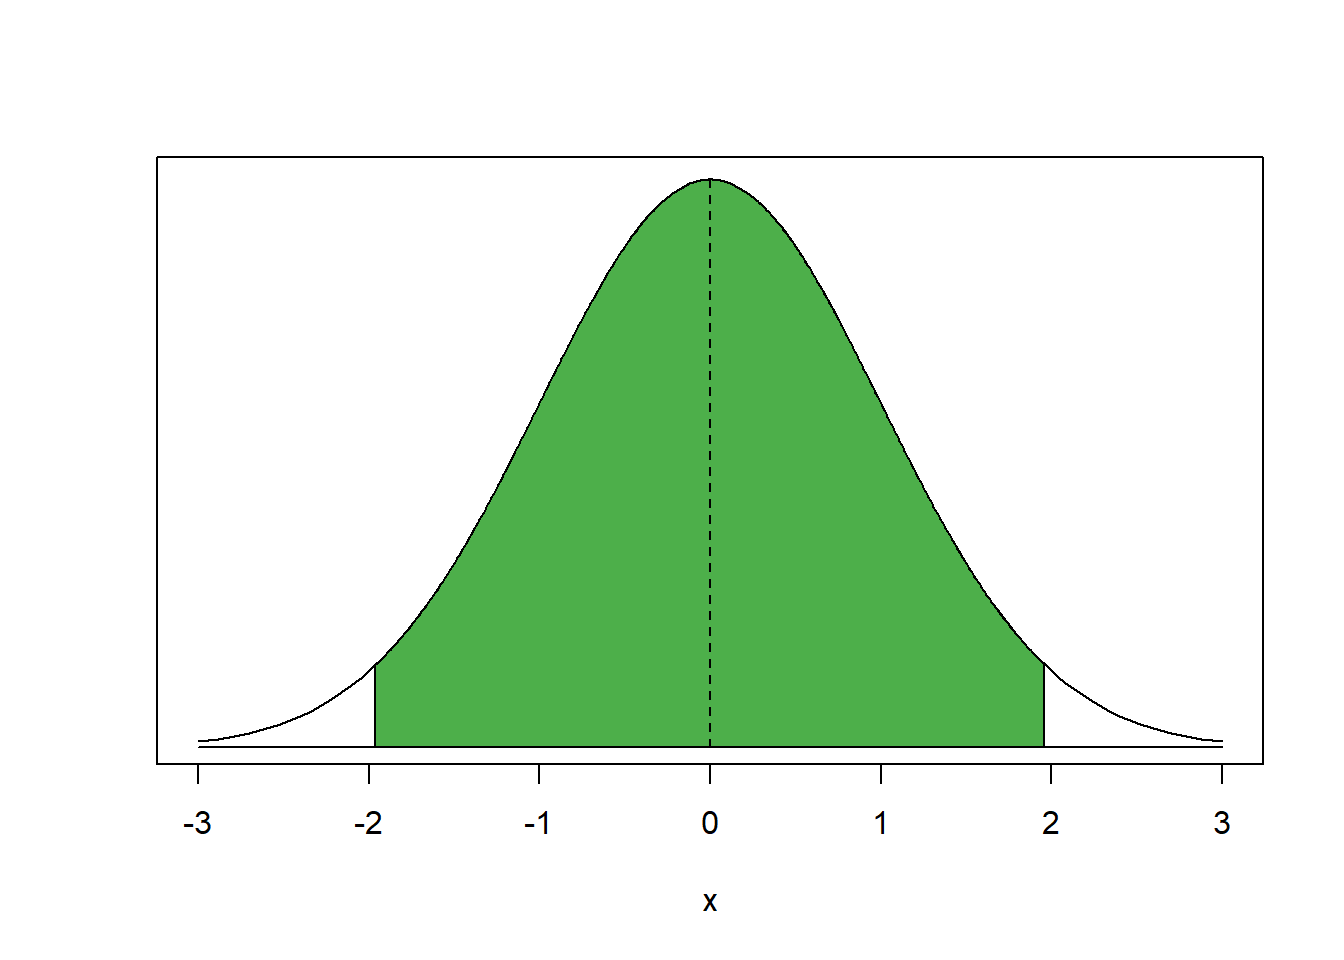
\includegraphics{statistics1_files/figure-latex/unnamed-chunk-175-1.pdf}

The green area under the curve covers 95 percent of all observations.
There are 2.5 percent in each tail. We reject the null hypothesis if our
estimate in is in the tails of the distribution. It must be further than
1.96 standard deviations from the mean. But how did we know that 95
percent of the area under the curve is within 1.96 standard deviations
from the mean.

We know from the cumulative probability. Separate the curve in you mind
into 3 pieces. The left tail covers 2.5 percent of the area under the
curve. The green middle bit covers 95 percent and the right tail again
2.5 percent. Now we do this as cumulative probabilities. The left tail
ends at 2.5 percent cumulative probability. The green area ends at 97.5
percent cumulative probability and the right tail ends at 100 percent.

The critical value is were the left tail ends or the right tail starts
(looking at the curve from left to right). Let's get the value where the
cumulative probability of where the left tail ends, i.e., is 2.5
percent.

\begin{Shaded}
\begin{Highlighting}[]
\CommentTok{# value for cumulative probability 95 percent in the standard normal distribution}
\KeywordTok{qnorm}\NormalTok{(}\FloatTok{0.025}\NormalTok{, }\DataTypeTok{mean =} \DecValTok{0}\NormalTok{, }\DataTypeTok{sd =} \DecValTok{1}\NormalTok{)}
\end{Highlighting}
\end{Shaded}

\begin{verbatim}
[1] -1.959964
\end{verbatim}

If you look at the x-axis of our curve that is indeed where the left
tail starts. We add a red dot to our graph to highlight it.

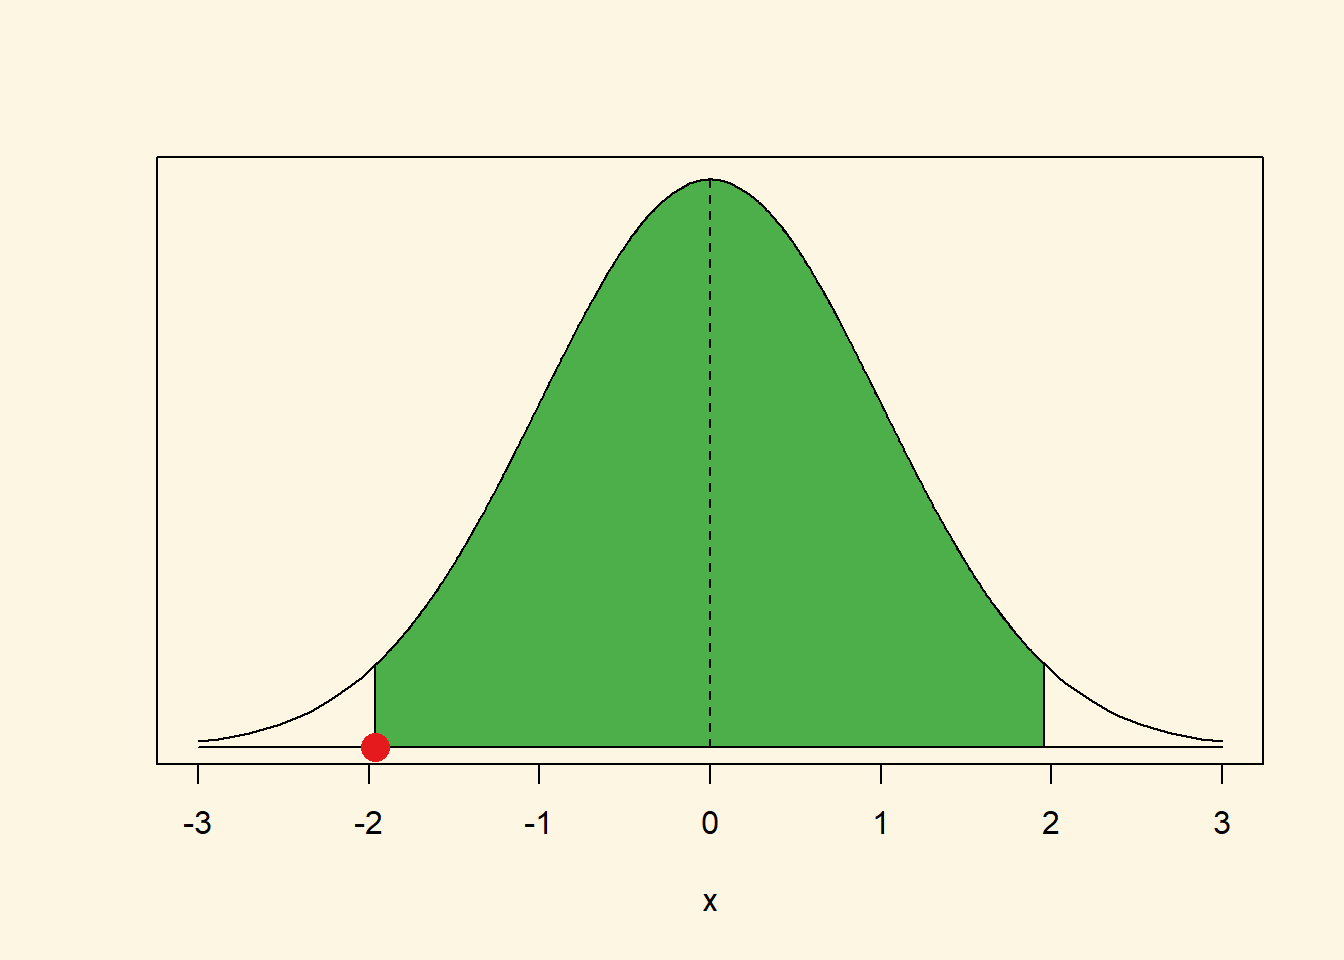
\includegraphics{statistics1_files/figure-latex/unnamed-chunk-177-1.pdf}

Now, let's get the critical value of where the right tail starts. That
is at the cumulative probability of 97.5 percent.

\begin{Shaded}
\begin{Highlighting}[]
\CommentTok{# value for cumulative probability 95 percent in the standard normal distribution}
\KeywordTok{qnorm}\NormalTok{(}\FloatTok{0.975}\NormalTok{, }\DataTypeTok{mean =} \DecValTok{0}\NormalTok{, }\DataTypeTok{sd =} \DecValTok{1}\NormalTok{)}
\end{Highlighting}
\end{Shaded}

\begin{verbatim}
[1] 1.959964
\end{verbatim}

As you can see, this is the same number only positive instead of
negative. That's always the case because the normal distribution is
symmetric. Let's add that point in blue to our graph.

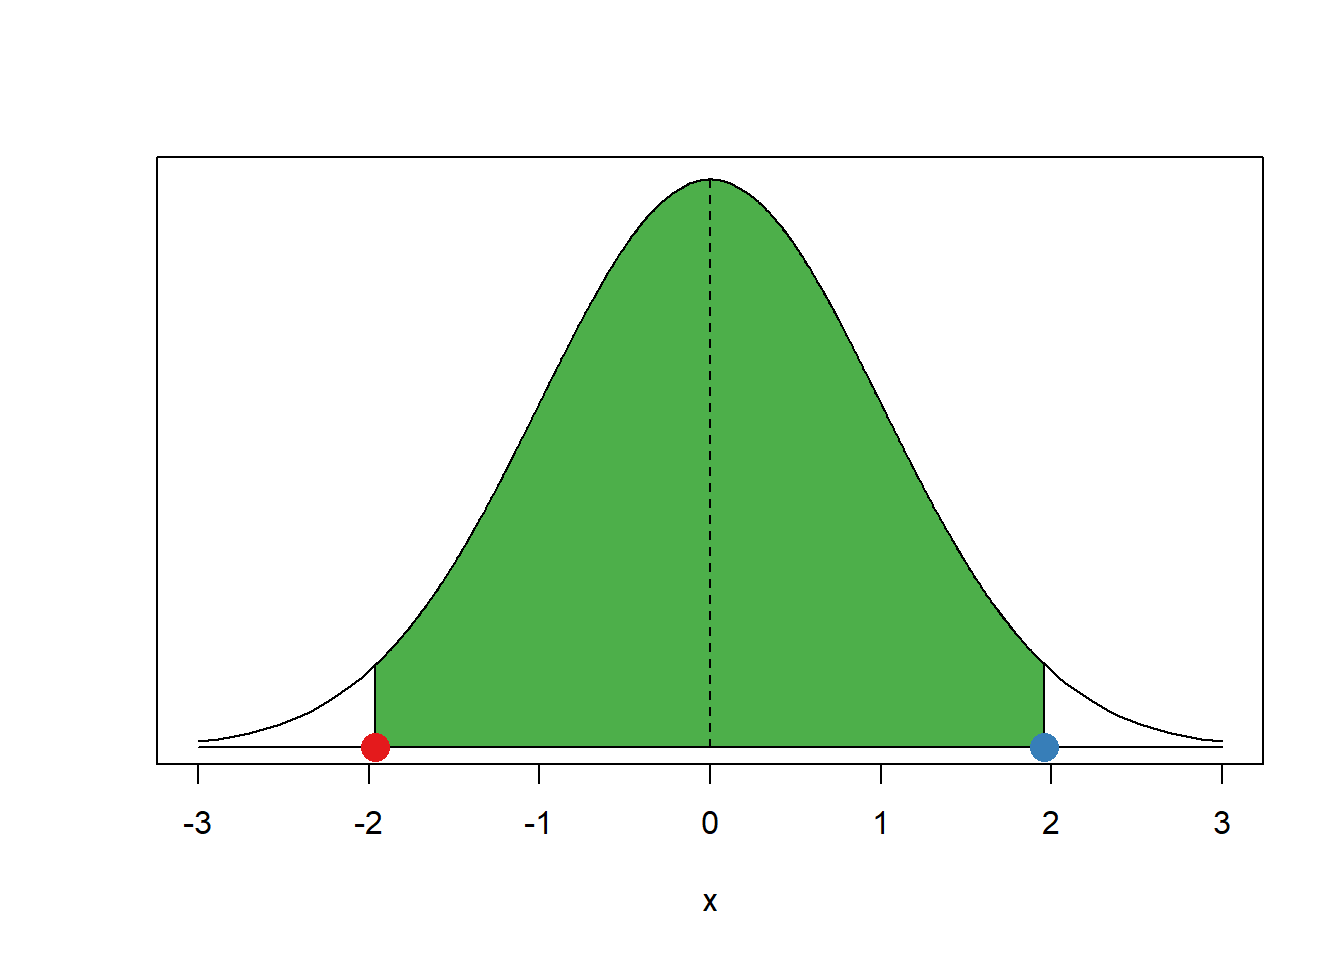
\includegraphics{statistics1_files/figure-latex/unnamed-chunk-179-1.pdf}

This is how we get the critical value for the 95 percent confidence
interval. As you can see our red and blue dots are the borders of the
green area, the 95 percent interval around the mean. You can get the
critical values for any other interval (e.g., the 99 percent interval)
similar to what we did just now.

We now do the same for the t distribution. In the t distribution, the
critical value depends on the shape of the t distribution which is
characterised by its degrees of freedom. Let's draw a t distribution
with 5 degrees of freedom.

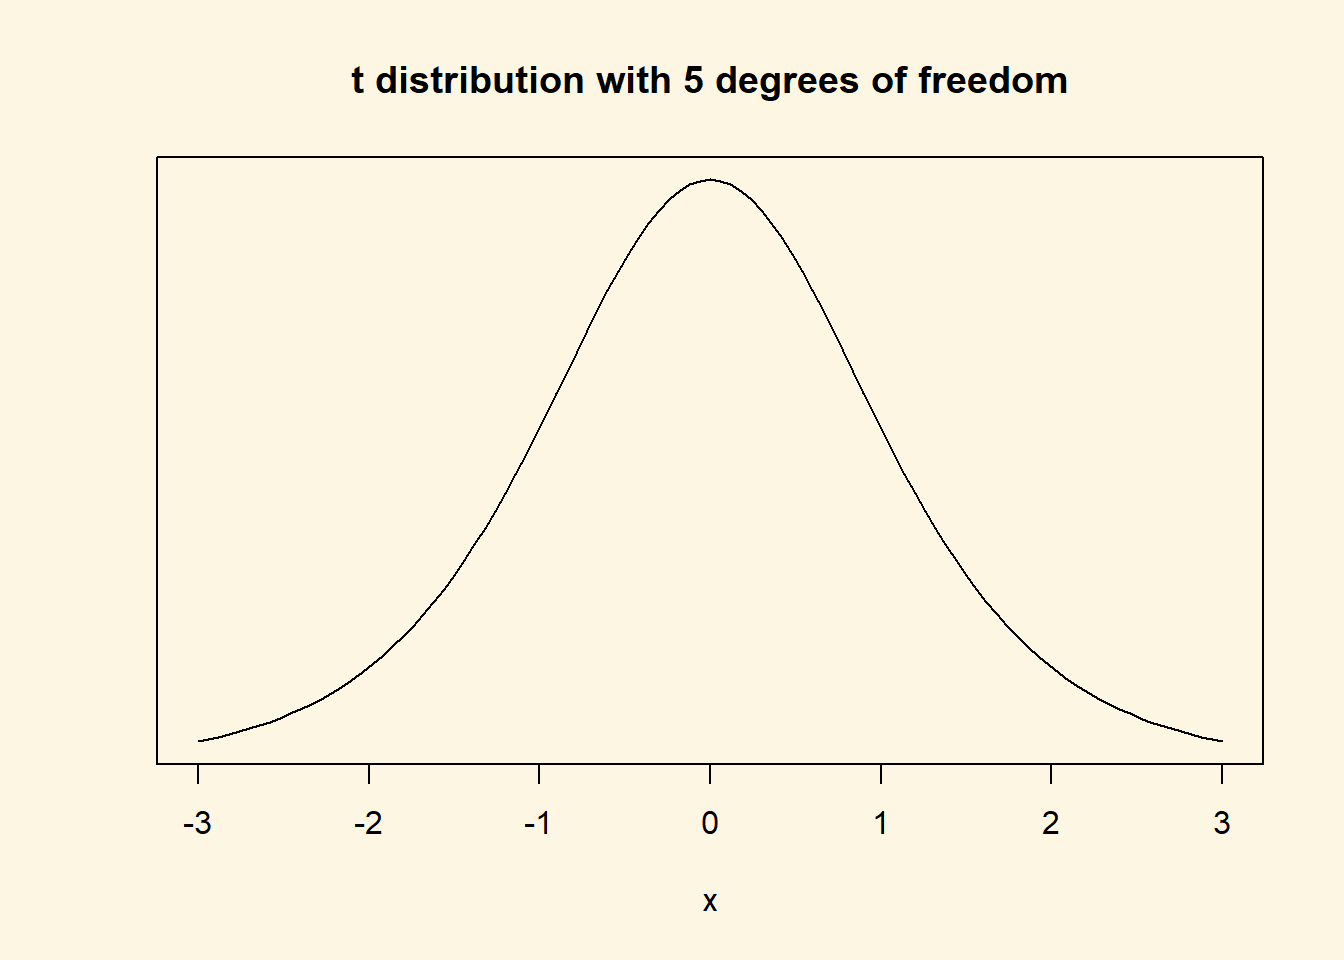
\includegraphics{statistics1_files/figure-latex/unnamed-chunk-180-1.pdf}

Although, it looks like a standard normal distribution, it is not. The t
with 5 degrees of freedom has fatter tails. We show this by overlaying
the t with a standard normal distribution.

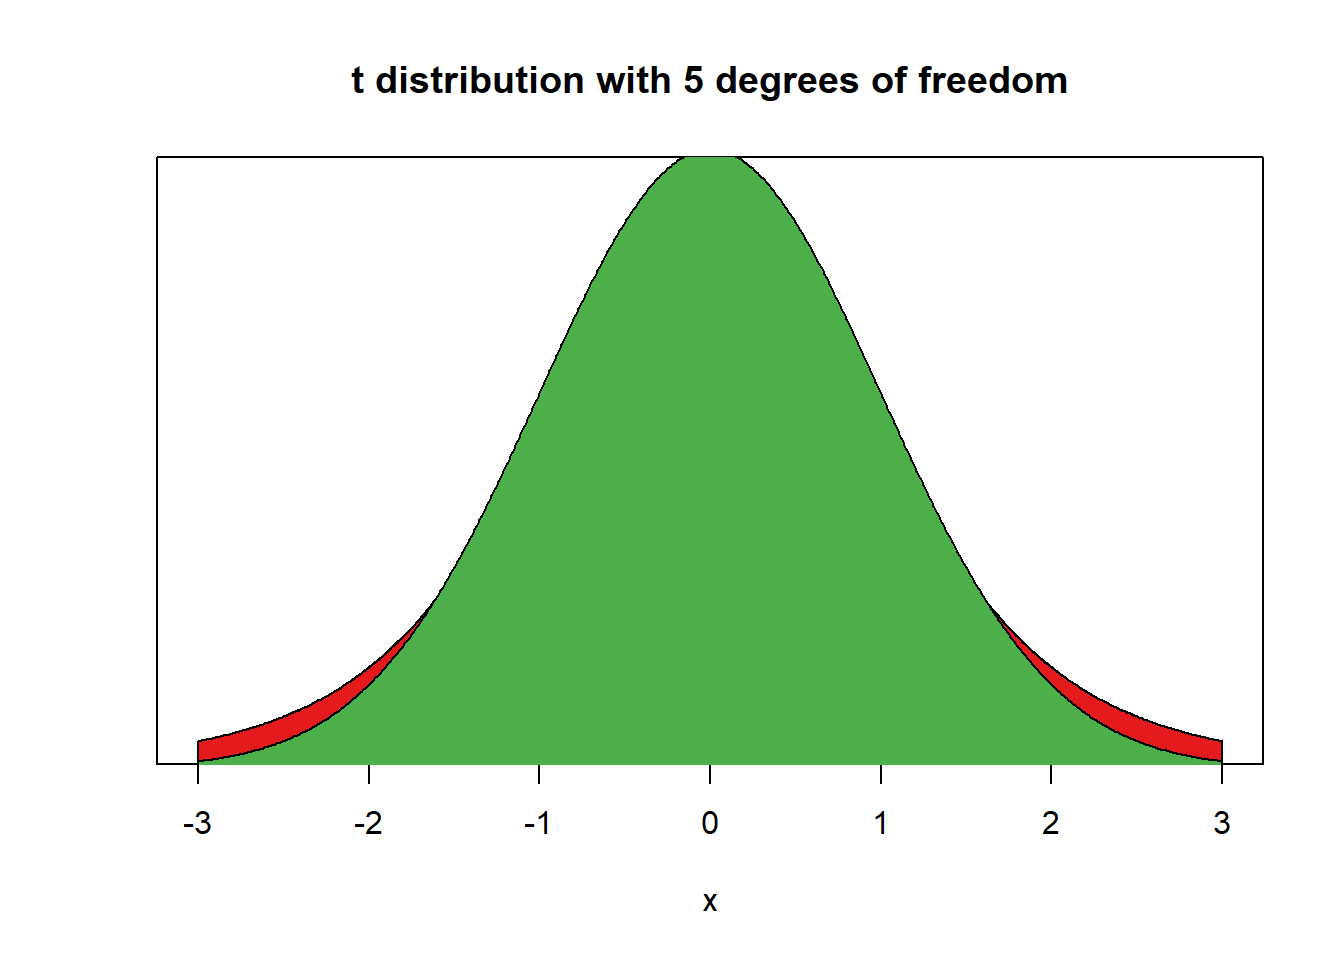
\includegraphics{statistics1_files/figure-latex/unnamed-chunk-181-1.pdf}

The red area is the difference between the standard normal distribution
and the t distribution with 5 degrees of freedom.

The tails are fatter and that means that the probabilities of getting a
value somewhere in the tails is larger. Lets calculate the critical
value for a t distribution with 5 degrees of freedom.

\begin{Shaded}
\begin{Highlighting}[]
\CommentTok{# value for cumulative probability 95 percent in the t distribution with 5 degrees of freedom}
\KeywordTok{qt}\NormalTok{(}\FloatTok{0.975}\NormalTok{, }\DataTypeTok{df =} \DecValTok{5}\NormalTok{)}
\end{Highlighting}
\end{Shaded}

\begin{verbatim}
[1] 2.570582
\end{verbatim}

See how much larger that value is than 1.96. Under a t distribution with
5 degrees of freedom 95 percent of the observations around the mean are
within the interval from negative 2.5705818 to positive 2.5705818.

Let's illustrate that.

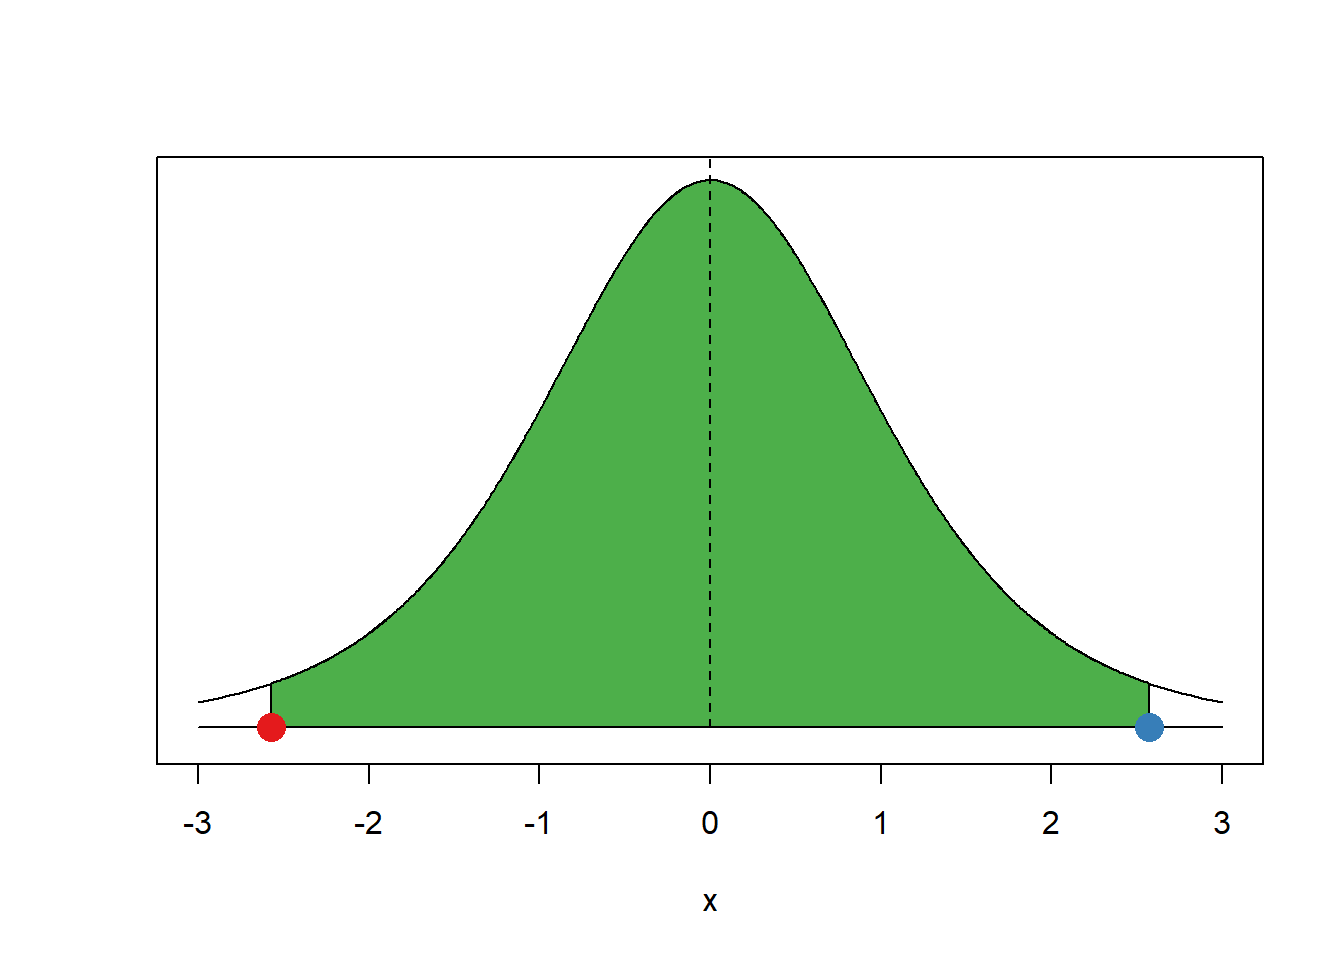
\includegraphics{statistics1_files/figure-latex/unnamed-chunk-183-1.pdf}

Remember the critical values for the t distribution are always more
extreme or similar to the critical values for the standard normal
distribution. If the t distribution has few degrees of freedom the
critical values (for the same percentage area around the mean) are much
more extreme. If the t distribution has many degrees of freedom, the
critical values are very similar.

\subsection{T-test (difference in
means)}\label{t-test-difference-in-means}

We are interested in whether there is a difference in income between
countries that have an independent judiciary and countries that do not
have an independent judiciary. Put more formally, we are interested in
the difference between two conditional means. Recall that a conditional
mean is the mean in a subpopulation such as the mean of income given
that the country has a free judiciary (conditional mean 1).

The t-test is the appropriate test statistic. Our interval-level
dependent variable is \emph{wealth} which is GDP per capita taken from
the World Development Indicators of the World Bank. Our binary
independent variable is \emph{h\_j} which is 1 if a country has a free
judiciary and 0 otherwise.

Let's check the summary statistics of our dependent variable GDP per
captia using the
\href{https://www.rdocumentation.org/packages/base/versions/3.4.1/topics/summary}{\texttt{summary()}}.

\begin{Shaded}
\begin{Highlighting}[]
\KeywordTok{summary}\NormalTok{(world.data}\OperatorTok{$}\NormalTok{wealth)}
\end{Highlighting}
\end{Shaded}

\begin{verbatim}
   Min. 1st Qu.  Median    Mean 3rd Qu.    Max. 
  226.2  1768.0  5326.1 10184.1 12976.5 63686.7 
\end{verbatim}

Someone claims that countries with free judiciaries are usually richer
than countries with controlled judiciaries. We know from the output of
the summary function that across all countries the average wealth is
10184.0910395 US dollars.

We use the \texttt{which()} function from last week again to identify
the row-numbers of the countries in our dataset that have free
judiciaries. The code below returns the row index numbers of countries
with free judiciaries.

\begin{Shaded}
\begin{Highlighting}[]
\KeywordTok{which}\NormalTok{(world.data}\OperatorTok{$}\NormalTok{h_j}\OperatorTok{==}\DecValTok{1}\NormalTok{)}
\end{Highlighting}
\end{Shaded}

\begin{verbatim}
 [1]   8   9  13  14  18  23  28  33  39  40  41  42  43  44  50  52  54
[18]  55  60  70  71  72  74  75  76  77  80  82  84  85  90  93  94 104
[35] 105 107 110 112 114 115 118 126 127 131 143 144 145 146 149 153 154
[52] 155 157 160 163 165 166 167 168 169 170 171 178
\end{verbatim}

Now, all we need is to index the dataset like we did last week. We
access the variable that we want (\emph{wealth}) with the dollar sign
and the rows in square brackets. The code below returns the per capita
wealth of the countries with a free judiciary.

\begin{Shaded}
\begin{Highlighting}[]
\KeywordTok{mean}\NormalTok{( world.data}\OperatorTok{$}\NormalTok{wealth[}\KeywordTok{which}\NormalTok{(world.data}\OperatorTok{$}\NormalTok{h_j}\OperatorTok{==}\DecValTok{1}\NormalTok{)])}
\end{Highlighting}
\end{Shaded}

\begin{verbatim}
[1] 17826.59
\end{verbatim}

Now, go ahead and find the mean per capita wealth of countries with
controlled judiciaries yourself.

\begin{Shaded}
\begin{Highlighting}[]
\KeywordTok{mean}\NormalTok{( world.data}\OperatorTok{$}\NormalTok{wealth[}\KeywordTok{which}\NormalTok{(world.data}\OperatorTok{$}\NormalTok{h_j}\OperatorTok{==}\DecValTok{0}\NormalTok{)])}
\end{Highlighting}
\end{Shaded}

\begin{verbatim}
[1] 5884.882
\end{verbatim}

Finally, we run the t-test.

\begin{Shaded}
\begin{Highlighting}[]
\CommentTok{# t.test for the difference between 2 means}
\KeywordTok{t.test}\NormalTok{(world.data}\OperatorTok{$}\NormalTok{wealth[}\KeywordTok{which}\NormalTok{(world.data}\OperatorTok{$}\NormalTok{h_j}\OperatorTok{==}\DecValTok{1}\NormalTok{)], }\CommentTok{# mean 1  }
\NormalTok{       world.data}\OperatorTok{$}\NormalTok{wealth[}\KeywordTok{which}\NormalTok{(world.data}\OperatorTok{$}\NormalTok{h_j}\OperatorTok{==}\DecValTok{0}\NormalTok{)], }\CommentTok{# mean 2}
       \DataTypeTok{mu =} \DecValTok{0}\NormalTok{, }\CommentTok{# difference under the null hypothesis}
       \DataTypeTok{alt =} \StringTok{"two.sided"}\NormalTok{,  }\CommentTok{# two sided test (difference in means could be smaller or larger than 0)}
       \DataTypeTok{conf =} \FloatTok{0.95}\NormalTok{) }\CommentTok{# confidence interval}
\end{Highlighting}
\end{Shaded}

\begin{verbatim}

    Welch Two Sample t-test

data:  world.data$wealth[which(world.data$h_j == 1)] and world.data$wealth[which(world.data$h_j == 0)]
t = 6.0094, df = 98.261, p-value = 0.00000003165
alternative hypothesis: true difference in means is not equal to 0
95 percent confidence interval:
  7998.36 15885.06
sample estimates:
mean of x mean of y 
17826.591  5884.882 
\end{verbatim}

Let's interpret the results you get from \texttt{t.test()}. The first
line tells us which groups we are comparing. In our example: Do
countries with independent judiciaries have different mean income levels
than countries without independent judiciaries?

In the following line you see the t-value, the degrees of freedom and
the p-value. Knowing the t-value and the degrees of freedom you can
check in a table on t distributions how likely you were to observe this
data, if the null-hypothesis was true. The p-value gives you this
probability directly. For example, a p-value of 0.02 would mean that the
probability of seeing this data given that there is no difference in
incomes between countries with and without independent judiciaries
\emph{in the population}, is 2\%. Here the p-value is much smaller than
this: 3.165e-08 = 0.00000003156!

In the next line you see the 95\% confidence interval because we
specified \texttt{conf=0.95}. If you were to take 100 samples and in
each you checked the means of the two groups, 95 times the difference in
means would be within the interval you see there.

At the very bottom you see the means of the dependent variable by the
two groups of the independent variable. These are the means that we
estimated above. In our example, you see the mean income levels in
countries were the executive has some control over the judiciary, and in
countries were the judiciary is independent.

\subsection{Estimating p values from t
values}\label{estimating-p-values-from-t-values}

Estimating the p value is the reverse of getting a critical value. We
have a t value and now we want to know what the probability is to get
such a value.

Let's say that we have a t distribution with 5 degrees of freedom. We
estimated a t value of 2.9. What is the corresponding p value?

\begin{Shaded}
\begin{Highlighting}[]
\NormalTok{(}\DecValTok{1} \OperatorTok{-}\StringTok{ }\KeywordTok{pt}\NormalTok{(}\FloatTok{2.9}\NormalTok{, }\DataTypeTok{df =} \DecValTok{5}\NormalTok{)) }\OperatorTok{*}\DecValTok{2}
\end{Highlighting}
\end{Shaded}

\begin{verbatim}
[1] 0.0337907
\end{verbatim}

This is the probability of getting a t value of 2.9 or larger (or -2.9
or smaller) given that the null hypothesis is true.
\texttt{pt(2.9,\ df\ =\ 5)} is the cumulative probability of getting a t
value of 2.9 or smaller. But we want the probability of getting a value
that is as large (extreme) as 2.9 or as small as -2.9. Therefore, we do
\texttt{1\ -\ pt(2.9,\ df\ =\ 5)}. We multiply by 2 to get both tails
\texttt{(1\ -\ pt(2.9,\ df\ =\ 5))*2}

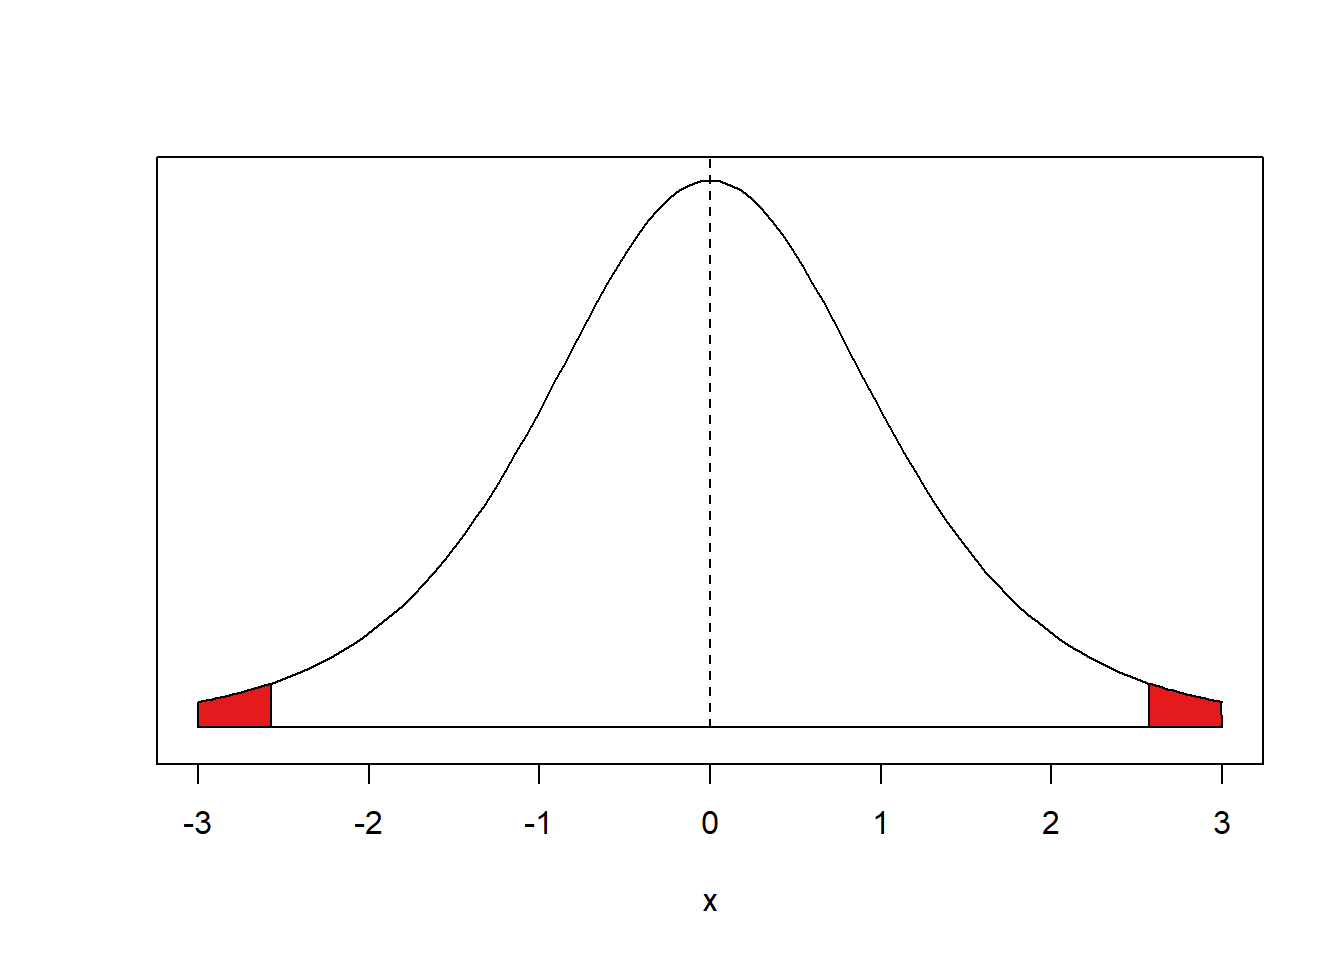
\includegraphics{statistics1_files/figure-latex/unnamed-chunk-190-1.pdf}

Clearly, the probability of getting such an extreme value (or something
larger) under the assumption that the null hypothesis is true is very
unlikely. The exact probability is \textasciitilde{}0.02 (2 percent).
We, therefore, think that the null hypothesis is false.

Let's estimate the p value in in a normal distribution (it's actually
better to always use the t distribution but the difference is negligible
if the t distribution has many degrees of freedom).

Let's take our earlier example where we had estimated a t value of
0.1995059. Our friend claimed world income is 10 000 per capita on
average and we estimated something slightly larger.

Let's check what the exact p value is in a normal distribution given a t
value of 0.1995059.

\begin{Shaded}
\begin{Highlighting}[]
\NormalTok{(}\DecValTok{1} \OperatorTok{-}\StringTok{ }\KeywordTok{pnorm}\NormalTok{(}\FloatTok{0.1995059}\NormalTok{))}\OperatorTok{*}\DecValTok{2}
\end{Highlighting}
\end{Shaded}

\begin{verbatim}
[1] 0.841867
\end{verbatim}

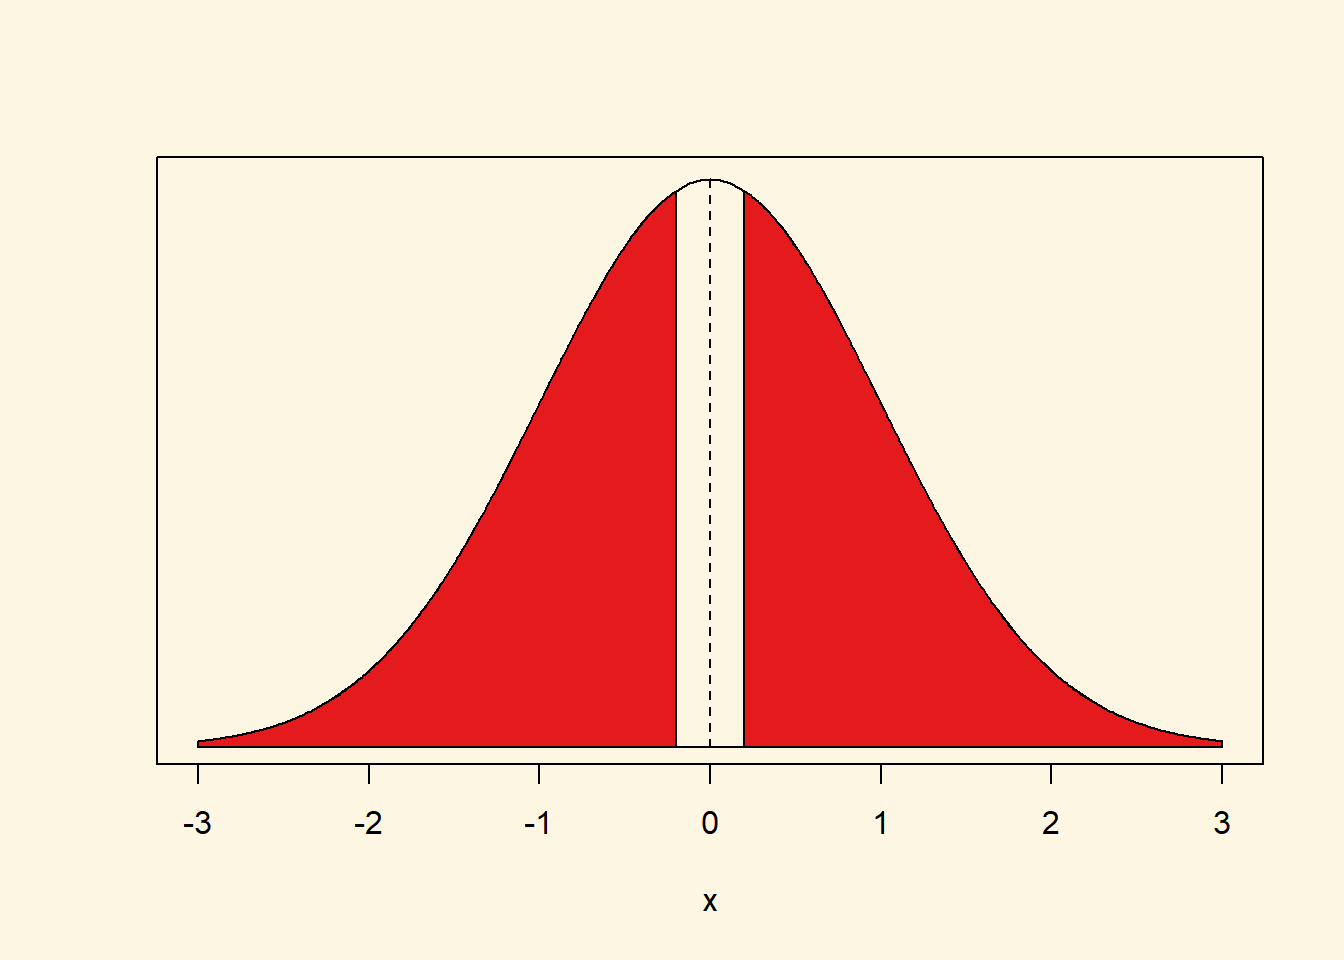
\includegraphics{statistics1_files/figure-latex/unnamed-chunk-192-1.pdf}

Clearly, it was not very unlikely to find a t value of 0.1995059 (that's
the absolute value, i.e., a t value of negative or postive 0.1995059)
under the assumption that the null hypothesis is true. Therefore, we
cannot reject the null. The probability is 0.84 (84 percent)---highly
likely.

\subsection{Exercises}\label{exercises-3}

\begin{enumerate}
\def\labelenumi{\arabic{enumi}.}
\tightlist
\item
  Create a new file called ``assignment2.R'' in your \texttt{PUBLG100}
  folder and write all the solutions in it.
\item
  Turn former colonies into a factor variable and choose appropriate
  labels.
\item
  How many countries were former colonies? How many were not?
\item
  Find the means of political stability in countries that (1) were
  former colonies, (2) were not former colonies.
\item
  Is the the difference in means statistically significant?
\item
  In layman's terms, are countries which were former colonies more or
  less stable than those that were not?
\item
  How about if we choose an alpha level of 0.01?
\item
  What is the level of measurement of the United Nations Development
  index variable \texttt{undp\_hdi}?
\item
  Check the claim that its true population mean is 0.85.
\item
  Calculate the t statistic.
\item
  Calculate the p value.
\item
  Construct a confidence interval around your mean estimate.
\item
  Discuss your findings in terms of the original claim. Interpret the t
  value, the p value, and the confidence interval.
\item
  Save the script that includes all previous tasks.
\item
  Source your script, i.e.~run the entire script all at once without
  error message.
\end{enumerate}

\subsection{Optional Exercises that require reading Extra Info
below}\label{optional-exercises-that-require-reading-extra-info-below}

\begin{enumerate}
\def\labelenumi{\arabic{enumi}.}
\tightlist
\item
  Create a scatter plot with latitude on the x-axis and political
  stability on the y-axis.
\item
  What is the correlation coefficient of political stability and
  latitude?
\item
  If we move away from the equator, how does political stability change?
\item
  Does it matter whether we go north or south from the equator?
\end{enumerate}

\subsection{Advanced Exercises}\label{advanced-exercises}

\begin{enumerate}
\def\labelenumi{\arabic{enumi}.}
\tightlist
\item
  Calculate the numerical difference in means (political stability
  conditional on colonialization) using the \texttt{means()} function.
\item
  Calculate the standard deviation of the difference in means (hint:
  using just the \texttt{sd()} function is incorrect in this context).
\item
  Is the difference in means more than 1.96 standard deviations away
  from zero? Interpret the result.
\item
  We claim the difference in means in terms of political stability
  between countries that were former colonies and those that were not is
  0.3. Check this hypothesis.
\item
  An angry citizen who wants to defund the Department of International
  Development (DFID) claims that countries that were former colonies
  have reached 75\% of the level of wealth of countries that were not
  colonised. Check this claim.
\end{enumerate}

\subsection{Extra Info}\label{extra-info}

When we want to get an idea about how two continuous variables change
together, the best way is to plot the relationship in a scatterplot. A
scatterplot means that we plot one continuous variable on the x-axis and
the other on the y-axis. Here, we illustrate the relation between the
human development index \texttt{undp\_hdi} and control of corruption
\texttt{wbgi\_cce}.

\begin{Shaded}
\begin{Highlighting}[]
\CommentTok{# scatterplot}
\KeywordTok{plot}\NormalTok{(world.data}\OperatorTok{$}\NormalTok{undp_hdi }\OperatorTok{~}\StringTok{ }\NormalTok{world.data}\OperatorTok{$}\NormalTok{wbgi_cce,}
  \DataTypeTok{xlim =} \KeywordTok{c}\NormalTok{(}\DataTypeTok{xmin =} \OperatorTok{-}\DecValTok{2}\NormalTok{, }\DataTypeTok{xmax =} \DecValTok{3}\NormalTok{),}
  \DataTypeTok{ylim =} \KeywordTok{c}\NormalTok{(}\DataTypeTok{ymin =} \DecValTok{0}\NormalTok{, }\DataTypeTok{ymax =} \DecValTok{1}\NormalTok{),}
  \DataTypeTok{frame =} \OtherTok{FALSE}\NormalTok{,}
  \DataTypeTok{xlab =} \StringTok{"World Bank Control of Corruption Index"}\NormalTok{,}
  \DataTypeTok{ylab =} \StringTok{"UNDP Human Development Index"}\NormalTok{,}
  \DataTypeTok{main =} \StringTok{"Relationship b/w Quality of Institutions and Quality of Life"}
\NormalTok{  )}
\end{Highlighting}
\end{Shaded}

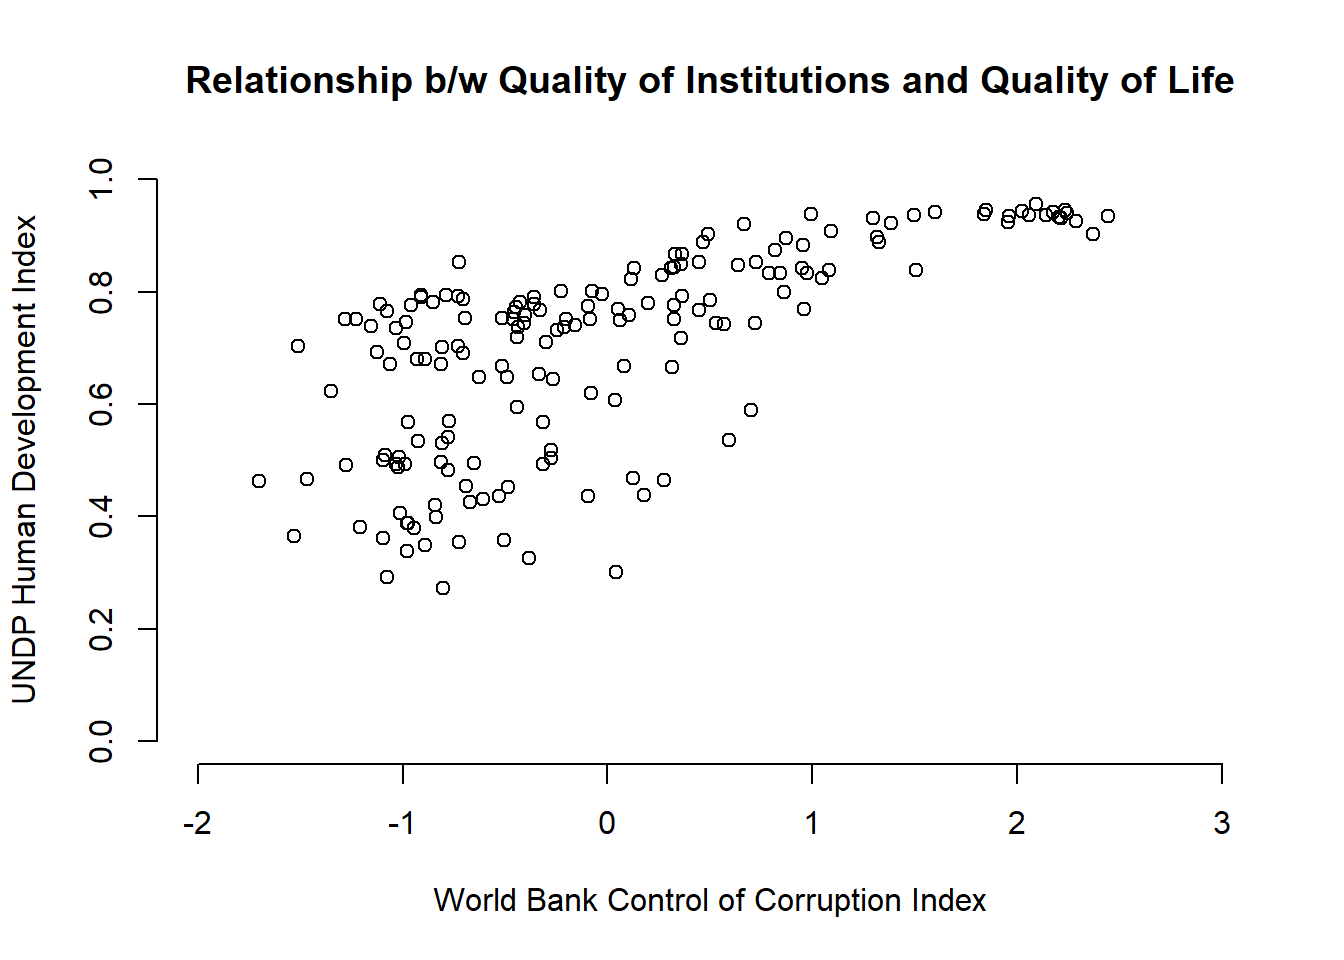
\includegraphics{statistics1_files/figure-latex/unnamed-chunk-193-1.pdf}

Sometimes people will report the correlation coefficient which is a
measure of linear association and ranges from -1 to +1. Where -1 means
perfect negative relation, 0 means no relation and +1 means perfect
positive relation. The correlation coefficient is commonly used as as
summary statistic. It's disadvantage is that you cannot see the
non-linear relations which can using a scatterplot.

We take the correlation coefficient like so:

\begin{Shaded}
\begin{Highlighting}[]
\KeywordTok{cor}\NormalTok{(}\DataTypeTok{y =}\NormalTok{ world.data}\OperatorTok{$}\NormalTok{undp_hdi, }\DataTypeTok{x =}\NormalTok{ world.data}\OperatorTok{$}\NormalTok{wbgi_cce, }\DataTypeTok{use =} \StringTok{"complete.obs"}\NormalTok{)}
\end{Highlighting}
\end{Shaded}

\begin{verbatim}
[1] 0.6813353
\end{verbatim}

\begin{longtable}[]{@{}ll@{}}
\toprule
\begin{minipage}[b]{0.12\columnwidth}\raggedright\strut
Argument\strut
\end{minipage} & \begin{minipage}[b]{0.78\columnwidth}\raggedright\strut
Description\strut
\end{minipage}\tabularnewline
\midrule
\endhead
\begin{minipage}[t]{0.12\columnwidth}\raggedright\strut
\texttt{x}\strut
\end{minipage} & \begin{minipage}[t]{0.78\columnwidth}\raggedright\strut
The x variable that you want to correlate.\strut
\end{minipage}\tabularnewline
\begin{minipage}[t]{0.12\columnwidth}\raggedright\strut
\texttt{y}\strut
\end{minipage} & \begin{minipage}[t]{0.78\columnwidth}\raggedright\strut
The y variable that you want to correlate.\strut
\end{minipage}\tabularnewline
\begin{minipage}[t]{0.12\columnwidth}\raggedright\strut
\texttt{use}\strut
\end{minipage} & \begin{minipage}[t]{0.78\columnwidth}\raggedright\strut
How R should handle missing values. \texttt{use="complete.obs"} will use
only those rows where neither \texttt{x} nor \texttt{y} is
missing.\strut
\end{minipage}\tabularnewline
\bottomrule
\end{longtable}


\end{document}
